% !TEX encoding = UTF-8
% !TEX program = pdflatex

\documentclass[a4paper]{article}
\usepackage[T1]{fontenc}
\usepackage[utf8]{inputenc}
\usepackage[italian]{babel}
\usepackage{booktabs}
\usepackage{caption}
\usepackage[table,xcdraw]{xcolor}
\usepackage{wrapfig}
\usepackage{graphicx}
\usepackage{fancyvrb}


\title{%
  Sistemi Operativi \\
  \large Riassunto del Corso - UniTN A.A. 2017/2018}

\author{Laura Scoccianti}

\begin{document}

\maketitle

\tableofcontents

\newpage

\section{Introduzione}

Un sistema operativo è un programma (o meglio, un insieme di programmi) che offre un ambiente per controllare e coordinare l'utilizzo dell'hardware da parte dei programmi applicativi. Tra le principali funzioni di un sistema operativo troviamo:
\begin{enumerate}
\item facilitare l'uso del computer per l'utente;
\item rendere efficiente l'uso dell'hardware;
\item evitare conflitti nell'allocazione delle risorse software e hardware;
\end{enumerate}
Alcuni Sistemi Operativi si progettano per essere di uso agevole, essere agevoli o per possedere entrambe le qualità. In ragione della sua complessità, un Sistema Operativo deve essere costruito gradualmente.

\subsection{Cos'è un Sistema Operativo?}

Un sistema di calcolo si può suddividere in quattro elementi:
\begin{enumerate}
\item Dispositivi fisici: CPU, memoria e dispositivi I/O
\item Programmi applicativi: definiscono il modo in cui si usano queste risorse per la risoluzione dei problemi degli utenti
\item Utenti: coloro che utilizzano il calcolatore
\item SO: controlla e coordina l’uso dei dispositivi da parte dei programmi applicativi
\end{enumerate}
In poche parole, un sistema di calcolo si può considerare come l’insieme dei suoi elementi fisici, programmi e dati. Il Sistema Operativo (\textit{SO}) offre gli strumenti per impiegare correttamente tali risorse fornendo un ambiente nel quale i programmi possono lavorare in modo utile, ovvero un'astrazione dei componenti dell'hardware. Il calcolatore vede il SO come un assegnatore di risorse, infatti esso le gestisce e le assegna ai programmi e agli utenti in modo tale che il sistema di calcolo operi in modo equo ed efficiente. Un SO è il solo programma che funziona sempre nel calcolatore (kernel).

\subsection{Storia dei sistemi operativi}

Possiamo suddividere la storia dei Sistemi Operativi in cinque generazioni. Nella prima (anni 50 circa), i calcolatori erano costituiti da enormi calcolatori a valvole senza sistema operativo. I programmi erano scritti su schede perforate e venivano azionati da \textit{operatori} tramite degli interruttori. Con l'evolversi della tecnologia, vennero sviluppate le prime "librerie" di funzioni comuni e i primi compilatori. Nella seconda generazione, vennero introdotti i transistor, riducendo enormemente le dimensioni dei calcolatori. Vennero inoltre introdotti le operazioni di batching e job sequencing, per raggruppare i programmi con esecuzione simile e delegandone il passaggio al sistema operativo. Venne inoltre introdotto un monitor residente nel "kernel" del sistema operativo, la sequenzializzazione e la sovrapposizione delle operazioni di I/O e CPU. 

Nella terza generazione, viene introdotta la multiprogrammazione (ovvero la competizione di job diversi per il tempo di CPU) e la divisione tra modalità \textbf{USER} (dove i job NON possono accedere all'I/O) e \textbf{KERNEL}. Per accedere alla modalità KERNEL vengono introdotti degli opportuni interrupt software per delegare l'accesso all'I/O da parte del sistema operativo.

Nelle ultime due generazioni, invece, i miglioramenti si sono focalizzati sulla progressiva specializzazione dei sistemi operativi per vari ambiti, ad esempio per i sistemi distribuiti, mobile ed embedded.



\subsection{Componenti di un sistema operativo}
Un Sistema Operativo fornisce un ambiente per l'esecuzione di programmi. Deve quindi essere in grado di gestire i processi, la memoria principale e secondaria, deve saper gestire l'I/O ed i files. 

\subsubsection{Gestione dei Processi}
Un processo è un programma in esecuzione, il quale necessita risorse e viene eseguito in maniera sequenziale (un'istruzione per volta). I processi possono essere catalogati in processi utente e processi di sistema.

Il sistema operativo è responsabile della creazione e distruzione dei processi, della loro eventuale sospensione e riesumazione e della fornitura di meccanismi necessari alla sincronizzazione e comunicazione tra molteplici processi.

\subsubsection{Gestione della Memoria Primaria}
La memoria primaria conserva i dati condivisi dalla CPU e dai dispositivi di I/O, pertanto un programma deve essere caricato in memoria per essere eseguito.

Il Sistema Operativo è responsabile della gestione dello spazio di memoria, ha il compito di decidere quale processo caricare in memoria (quando esiste spazio disponibile) ed esegue l'allocazione e il rilascio dello spazio di memoria.

\subsubsection{Gestione della memoria secondaria}
La memoria primari è volatile e di dimensioni relativamente ridotte, è quindi indispensabile questo secondo tipo di memoria, tipicamente costituita da uno o più dischi magnetici, per mantenere grandi quantità di dati in modo permanente.

Il Sistema Operativo è responsabile della gestione dello spazio libero, allocazione dello spazio e scheduling degli accessi su disco.

\subsubsection{Gestione dell'I/O}
Per questioni di sicurezza, l'utente non può controllare direttamente i dispositivi di I/O, i quali sono ``nascosti'' dal Sistema Operativo. Quest'ultimo deve quindi fare da tramite tra l'utente e i vari dispositivi, avendo a disposizione un sistema per accumulare gli accessi ai dispositivi (buffering) e device drivers specifici.

\subsubsection{Gestione dei Files}
Formalmente, un file è un'astrazione logica per rendere conveniente l'uso della memoria non volatile. Le informazioni vengono memorizzate su supporti fisici diversi (dischi, DVD, memory-stick, ...) controllati da drivers con caratteristiche diverse.

Il S.O. è responsabile della creazione e cancellazione di files e directories, del supporto di primitive per la gestione di files e directories (copia, sposta, modifica, ...), della corrispondenza tra file e spazio fisico su disco e del salvataggio delle informazioni a scopo di backup.

\subsubsection{Protezione}
Quando diversi processi vengono eseguiti in maniera concorrenziale, non dovrebbe essere possibile, per uno qualsiasi di loro, interferire con un qualsiasi altro o con lo stesso Sistema Operativo. La protezione è quindi il controllo dell'accesso alle risorse da parte di processi e utenti. 

Un Sistema Operativo è quindi responsabile della definizione dei controlli da imporre, della fornitura di strumenti per verificare le politiche di accesso e dell'autorizzazione all'accesso (solitamente tramite password).

\subsubsection{Rete}
Si definisce Sistema Distribuito una collezione di elementi di calcolo che non condividono né la memoria né un clock, le risorse di calcolo sono quindi connesse tramite una rete. Un tale sistema fornisce una maggiore velocità, potenza, funzionalità e affidabilità all'utente.

Il compito del Sistema Operativo in questo caso è quello di gestire, attraverso i protocolli di rete, i processi distribuiti, la memoria distribuita e l'intero file system distribuito. 

\subsubsection{Interprete dei comandi (Shell)}
La maggior parte dei comandi vengono forniti dall'utente al Sistema Operativo tramite ``'istruzioni di controllo''', le quali permettono di creare e gestire processi, gestire l'I/O, il disco, la memoria il file system, le protezioni e la rete. Il programma che legge ed interpreta questi comandi è l'interprete dei comandi.
\paragraph{L'interprete}
Il compito principale dell'interprete è prendere i comandi specificati dall'utente ed eseguirli. Esso stesso è già in possesso del codice di tali comandi, cui l'utente si riferisce con nomi predefiniti (ad esempio, il comando \texttt ls in una shell Linux).
\paragraph{L'interfaccia utente}
L'interprete può fornire diversi tipi di interfaccia utente: Command-Line (CLI), Graphics User Interface (GUI), Batch
\subparagraph{CLI} Permette di digitare direttamente comandi testuali, è spesso implementata nel kernel o alternativamente come programma di sistema e si può presentare in diverse varianti (dette shells).
\subparagraph{Interfaccia Utente - GUI} Generalmente il desktop, in combinazione con mouse e tastiera, è considerato la metafora della GUI.

\subsection{System Calls}
Le chiamate di sistema costituiscono l'interfaccia tra i processi e i servizi offerti dal Sistema Operativo. Queste chiamate sono generalmente disponibili come routines scritte in linguaggi di alto livello come C o C++, ma non è raro trovarne alcune scritte addirittura in assembler.

Ogni programma, anche il più (apparentemente) banale, durante l'esecuzione arriva ad utilizzare decine di system calls, una per ogni ``piccola'' operazione necessaria.\newline
La realizzazione di un programma, tuttavia, si basa sulle API (Application Programming Interface), cioè set di funzioni disponibili in un dato contesto le quali a loro volta si occupano di invocare le vere system calls, solitamente diverse per ogni sistema, garantendo la portabilità delle applicazioni.

Ogni system call è identificata da un numero e l'interfaccia alle chiamate di sistema mantiene una tabella indicizzata secondo questi numeri. L'interfaccia alle chiamate di sistema quindi invoca la call utilizzata, nel kernel del Sistema Operativo, e ritorna quindi lo stato della system call e gli eventuali valori di ritorno. Il chiamante non ha chiaramente bisogno di conoscere nulla di come la system call sia implementata o di cosa faccia durante l'esecuzione, è quindi fornito un livello intermedio per mascherare i dettagli implementativi di un Sistema Operativo: le API (già citate).

Le opzioni per la comunicazione tra il Sistema Operativo e un processo sono molteplici: è possibile passare i parametri delle system calls tramite i registri (veloci ma poco capaci), tramite lo stack del programma o memorizzandoli in una tabella in memoria, per poi passare l'indirizzo della tabella in un registro o nello stack.

\subsection{Programmi di sistema}
I programmi di sistema, conosciuti anche come utilità di sistema (system utilities), forniscono un ambiente funzionale per lo sviluppo e l'esecuzione di programmi da parte dell'utente, il quale generalmente non ha accesso diretto alle system call. Alcuni di questi programmi sono semplici system call interfaces, mentre altri sono considerevolmente più complessi. 

Si distinguono le seguenti categorie di programmi di sistema:
\begin{enumerate}
\item Gestione e manipolazione dei files (creare, copiare, cancellare, spostare, ecc.)
\item Informazioni sullo stato di sistema (data, memoria libera, ecc.)
\item Editor di testo
\item Supporto ai linguaggi di programmazione (compilatori, assemblatori, debugger, interpreti, sia integrati nel sistema che scaricabili separatamente)
\item Interprete dei comandi
\item Programmi di gestione della rete
\item Servizi di background e utility varie (per svariati scopi)
\end{enumerate}

Accanto ai programmi di sistema troviamo gli application programs, utili per risolvere svariati problemi. Appartengono a questa categoria i browser web, gli editor di testi complessi, i gestori per fogli di calcolo, sistemi per databases, giochi, eccetera.

\newpage
\section{Architettura di un Sistema Operativo}
Sistemi estesi e complessi come i moderni Sistemi Operativi devono essere progettati seguendo principi di progettazione tali darendere possibile il loro corretto ed efficiente funzionamento e la possibilità di introdurre modifiche nel tempo (ad esempio:aggiornamenti). Un principio molto importante è la separazione tra policy (cosa deve essere fatto?) e i meccanismi (come farlo?) la sua importanza risiede nella maggior flessibilità conferita al sistema, soprattutto se le policy tendono a variare nel tempo.
Altri due principi rilevanti sono il KISS (Keep It Small and Simple) e il POLA (Principle of the Least Privileges), il qualeafferma che ogni componente deve avere solo i privilegi necessari ad eseguire la sua funzione e nulla più, che fra l'altro èalla base dell'affidabilità e della sicurezza di un Sistema Operativo.

\subsection{Struttura di un Sistema Operativo}
Le componenti di un sistema possono essere interconnesse tra loro e combinate nel kernel secondo strutture diverse. Passiamo orain rassegna le diverse possibilità.

\subsubsection{Sistemi a struttura semplice}
Molti Sistemi Operativi non hanno una struttura ben definita. Spesso questi sistemi sono nati per essere ``piccoli'', semplici elimitati e poi sono stati evoluti oltre il loro scopo originario (MS-DOS ne è un esempio), ma all'inizio di era badato solo aridurre i costi di sviluppo e manutenzione. 

Sistemi come MS-DOS erano stati scritti per fornire la maggior funzionalità nel minor spazio possibile, quindi non si era troppobadato alla divisione in moduli o alla creazione secondo una ben determinata struttura, con una conseguente poco chiaradefinizione dei livelli di funzionalità e delle interfacce. Ovviamente, MS-DOS era anche limitato dall'hardware disponibileall'epoca della sua nascita. Poiché l'Intel 8088 per cui era stato scritto non prevedeva una dual mode, né tantomeno unaprotezione dell'hardware, gli sviluppatori di MS-DOS non ebbero altra scelta che lasciare che fosse possibile accedereall'hardware di base.

Anche UNIX rappresenta un esempio di sistema a struttura semplice, ancora una volta per via delle limitate funzionalitàhardware. Consisteva però di due parti separate: il kernel e i programmi di sistema. Il kernel è poi ulteriormente separato inuna serie di interfacce e driver di device, aggiunti e sviluppati durante gli anni durante l'evoluzione di UNIX.Tradizionalmente, il kernel forniva il file system, la scheduling della CPU, la gestione della memoria e altre funzioni disistema tramite system calls. In sostanza, un enorme quantità di funzionalità combinata in un unico livello. Una tale strutturamonolitica era difficile da implementare e mantenere.

\subsubsection{Sistema a livelli}
Con un appropriato supporto hardware, un Sistema Operativo può essere spezzato in pezzi più piccoli e più appropriati di quellipermessi da MS-DOS e dai primi sistemi UNIX. Esistono vari metodi per modularizzare un sistema. 

In questa categoria, il Sistema Operativo è visto a livelli: il più basso (livello 0) è l'hardware, mentre il più alto (livelloN) è l'interfaccia utente. 
Il vantaggio principale risiede nella semplicità di costruzione e debugging. Ogni livello è implementato in modo da poter usare solo funzioni fornite dai livelli inferiori, mentre definisce precisamente il tipo di servizio e l'interfaccia verso il livello superiore nascondendone l'implementazione. Tale struttura semplifica il debugging poiché il primo livello può essere debuggato senza troppe preoccupazioni sul resto del sistema, essendo subito al di sopra dell'hardware. Passando al livello superiore, si può assumere che tutti i servizi forniti dal livello precedente siano corretti, quindi eventuali errori possono trovarsi solo nel livello attuale, e così via per ogni livello.

La maggiore difficoltà con l'approccio a livelli consiste nel definire appropriatamente gli strati. Poiché un livello può usare solo servizi dei livelli sottostanti, è necessario pianificare tutto con attenzione. Ad esempio, il device driver per il backing store (lo spazio su disco usato da algoritmi della memoria virtuale) deve per forza essere a un livello necessariamente più basso di quello che implementa le routines di gestione della memoria, proprio perché queste richiedono di poter usare il backing store. Risulta quindi evidente che un sistema di questo tipo non è caratterizzato da una grande portabilità, dato che le funzionalità dipendenti dall'architettura sono sparse su vari livelli, che potrebbero essere necessariamente diversi per macchine costruite diversamente.

Un altro problema è la minor efficienza: ogni strato aggiunge overhead alle system calls, cioè a ogni livello i parametri passati potrebbero essere modificati, potrebbero essere aggiunti altri dati, e così via.

Un primo esempio di sistema a livelli è stato THE (Dijkstra 1968), sviluppato per sistemi batch per scopi accademici, era costituito da un insieme di processi cooperanti sincronizzati tramite semafori.

\subsubsection{Microkernel}
In questo approccio, tutti i componenti non essenziali vengono rimossi dal kernel e vengono implementati come programmi di sistema o addirittura programmi utente. Tipicamente, i microkernels forniscono servizi di gestione dei processi e della memoria, in aggiunta a quelli per la comunicazione.

La funzione principale di un microkernel è quella di permettere la comunicazione tra il programma client e i vari servizi a loro volta attivi nello user space. La comunicazione inter-processo è svolta tramite il passaggio di messaggi (message passing). Il programma client e il servizio, quindi, non comunicano mai direttamentente. Piuttosto, comunicano indirettamente scambiandosi messaggi con il microkernel.

L'approccio con microkernel permette di sviluppare sistemi facilmente espandibili e altamente portabili, oltre che più sicuri e affidabili. Tuttavia, presentano un overhead significativo dovuto alla chiamata continua di system call (con passaggio alla modalità kernel).

\subsubsection{Virtual Machine}
Questo approccio, pensato per offrire un sistema timesharing ``multiplo'', è un'estremizzazione dell'approccio a livelli. La virtualizzazione è una tecnologia che permette ai Sistemi Operativi di essere eseguiti come se fossero applicazioni, contemporaneamente. L'uso di macchina virtuali rende inoltre ogni sistema portabile poiché, anche se nativamente studiato per funzionare su un certo hardware, essendo il kernel ``appoggiato'' sulla Virtual Machine (e non direttamente sull'hardware), non ha problemi a girare su un hardware diverso. Inoltre, uuna macchina virtuale può supportare molti sistemi operativi contemporaneamente, senza che questi si disturbino l'un l'altro. Risulta quindi possibile fare su una sola macchina quello che magari fino a qualche anno fa richiedeva l'utilizzo di tante macchine diverse.

Una Virtual Machine può essere implementata due modi: con un Hypervisor di livello 1 (dove abbiamo un monitor implementato direttamente sopra l'hardware che gestisce macchine virtuali multiple alla volta) e di livello 2, dove è la macchina virtuale stessa a essere gestita all'interno di un sistema operativo nativo e residente sulla macchina.

Un tale sistema soffre però di problemi di prestazioni: in un qualsiasi sistema di emulazione, ogni istruzione a livello macchina che può essere nativamente eseguita nel sistema sorgente, deve essere tradotta nella funzione equivalente del sistema di destinazione, spesso rappresentata da molte più istruzioni. Inoltre è necessario gestire una dual mode virtuale: il sistema di gestione delle Virtual Machines esegue in kernel mode, mentre la VM esegue in user mode. 

\subsection{Conclusioni: implementazione di un Sistema Operativo}
Tradizionalmente i Sistemi Operativi erano scritti in linguaggio assembler. Ora, sono sviluppati in linguaggi di alto livello, quali C e C++, poiché l'implementazione risulta più rapida, il codice rimane molto più compatto, quindi più facile da capire e mantenere e sono più facilmente portabili.

\newpage
\section{Processi e Threads - Parte 1 (Processi)}

I primi computer permettevano l'esecuzione di un solo programma alla volta. Questo programma aveva completo controllo del sistema e poteva accedere a tutte le risorse del sistema. Al contrario, i moderni computer permettono il caricamento il memoria e l'esecuzione concorrenziale di molti programmi. Questa evoluzione ha richiesto un controllo più serrato e una netta divisione tra i vari programmi. Da qui nasce il concetto di processo, che è un programma in esecuzione. Un sistema consiste dunque in una collezione di processi.

\subsection{Cos'è un processo}
Si è definito un processo come un programma in esecuzione, ma è molto più del semplice codice del programma. Un qualsiasi processo consiste di: 
\begin{enumerate}
\item Istruzioni, cioè il codice del programma
\item Dati, ad esempio le variabili globali
\item Stack, il quale contiene le variabili locali e le chiamate a procedura e i relativi parametri
\item Heap, ovvero la memoria allocata dinamicamente durante l'esecuzione
\item Attributi: id, stato, controllo, program counter (ovvero il valore che indica l'attività corrente), valori dei registri, informazioni sulla memoria, informazioni sullo stato dell'I/O, sull'utilizzo del sistema (CPU) e di scheduling (ad esempio: priorità).
\end{enumerate} 

\subsection{Stato di un processo}
Durante la sua esecuzione, un processo evolve attraverso diversi stati. Un processo potrebbe trovarsi in uno dei seguenti stati:
\begin{enumerate}
\item New (Nuovo) : creazione del processo
\item Running (In esecuzione)
\item Waiting (In attesa) : il processo aspetta che succeda un determinato evento, ad esempio un I/O.
\item Ready : il processo è pronto ad essere assegnato al processore
\item Terminated (Finito) : il processo ha terminato la sua esecuzione e ha restituito risorse
\end{enumerate}

Bisogna notare che un solo processo alla volta può essere in esecuzione su un processore, ma molti processi potrebbero essere ready o waiting.

\subsection{Scheduling dei processi}
Dato che un solo processo per volta può utilizzare la CPU, la selezione del processo da eseguire in un determinato momento è molto importante. Gli obiettivi da conseguire sono: la multiprogrammazione e il time-sharing. Con la multiprogrammazione si vuole massimizzare l'uso della CPU, mantenendo più di un processo in memoria, mentre con time-sharing si indica la volontà di commutare frequentemente la CPU tra processi, di modo che ognuno di essi creda di avere la CPU tutta per sé.

La selezione del processo cui allocare la CPU spetta agli scheduler. \newline
Il long-term scheduler, o job scheduler, seleziona quali processi devono essere trasferiti dalla memoria alla coda dei processi pronti. Questo scheduler controlla il gradi di multiprogrammazione, ovvero il numero di processi in memoria. Se il grado è stabile, la il tasso di creazione medio dei processi dovrebbe essere circa uguale al tasso medio di terminazione. Il long-time scheduler non esegue frequentemente, quindi può permettersi di impiegare un tempo discreto per prendere le sue decisioni. Lo short-term scheduler, o CPU scheduler, seleziona i processi da eseguire tra quelli nella ready queue e alloca la CPU di conseguenza. Un processo potrebbe eseguire per pochi millisecondi prima di richiedere un I/O, lo short-term scheduler deve quindi essere eseguito frequentemente (per non lasciare la CPU inutilizzata, in questo specifico scenario) e deve essere particolarmente veloce.

In generale, i processi possono essere descritti come I/O-bound o CPU-bound. Un processo I/O-bound spende la maggior parte del tempo completando operazioni di I/O piuttosto che computazioni. Un processo CPU-bound, al contrario, raramente richiede I/O e sfrutta la maggior parte del tempo eseguendo computazioni, utilizzando quindi pochi e lunghi burst di CPU, al contrario dei frequenti e corti utilizzati dal primo tipo di processi. Di rilevante importanza è quindi il lavoro del long-term scheduler, il quale deve essere in grado di selezionare il giusto mix tra i due tipi di processi: se ci sono troppi I/O-bound, la ready queue sarà spesso vuota, al contrario, sarà spesso troppo piena se ci sono troppi CPU-bound.

\subsection{Code di scheduling}
Quando un processo entra nel sistema, è inserito nella job queue, che contiene tutti i processi del sistema. I processi che risiedono in memoria e sono pronti ad eseguire vengono inseriti nella ready queue. Quando a un processo viene finalmente allocata la CPU, potrebbe eseguire per del tempo e poi lasciarla, oppure essere interrotto o in attesa di un certo evento. La lista dei processi che stanno aspettando un particolare dispositivo di I/O si chiama device queue (coda di dispositivo). 
\subsubsection{Operazione di dispatch}
Un processo inizialmente è inserito nella ready queue. Esso aspetta qui finché non viene selezionato dallo short-term scheduler e il dispatcher non gli assegna il controllo della CPU. Le operazioni compiute dal dispatcher sono:
\begin{enumerate}
\item Cambio di contesto: viene salvato il Process Control Block (serie di informazioni sul processo) del processo che esce e viene caricato il PCB del processo entrante
\item Passaggio alla modalità utente: all'inizio della fase di dispatch il processo si troca in modalità kernel
\item Salto all'istruzione da eseguire del processo appena arrivato nella CPU
\end{enumerate}

\subsubsection{Cambio di contesto}
Come già precedentemente menzionato, gli interrupt forzano la CPU a scambiare l'esecuzione della task corrente con l'esecuzione di una routine kernel. Quando accade un interrupt, il sistema ha bisogno di salvare il contesto corrente del processo in esecuzione sulla CPU, così da poterlo riesumare quando le condizioni saranno di nuovo favorevoli. Il contesto è rappresentato dal Process Control Block del processo in questione. Esso include i valori dei registri della CPU, lo stato del processo e le informazioni di gestione della memoria. Generalmente viene salvato anche lo stato della CPU. \newline
Allocare la CPU a un altro processo richiede il salvataggio dello stato della CPU e la riesumazione dello stato di un processo diverso. Questa serie di operazioni è nota come cambio di contesto (context switch). \newline
Il tempo necessario al cambio di contesto è puro sovraccarico per il sistema poiché questo non compie alcun lavoro utile durante la commutazione. La durata del context switch è fortemente dipendente dall'hardware, ad esempio, in architetture con molti registri a disposizione il cambio è più veloce perché il sistema può salvare e recuperare le informazioni sul vari processi direttamente da lì, ma se i processi sono in numero maggiore rispetto ai registri, tutti i dati dovranno essere ogni volta scambiati da registri a memoria e da memoria a registri, risultato in un grande dispendio di tempo.

\subsection{Operazioni sui processi}
Nella maggior parte dei sistemi, i processi possono eseguire concorrenzialmente e possono essere creati e distrutti dinamicamente.

\subsubsection{Creazione di un processo}
Durante la sua esecuzione, un processo può creare molti nuovi processi, chiamati processi figli. La quasi totalità dei sistemi operativi identifica i processi in base al process id (pid). Il pid costituisce un valore unico per ogni processo nel sistema e può essere usato come indice per accedere ai vari attributi di un processo nel kernel. \newline
In generale, quando un processo crea un figlio, il nuovo processo avrà bisogno di certe risorse per completare le sue task. Il processo figlio potrebbe ottenere le risorse direttamente dal Sistema Operativo o dal padre (per spartizione o per condivisione). \newline
Quando un processo crea un nuovo processo, esistono due possibilità per l'esecuzione: sincrona, ovvero il padre aspetta la terminazione dei figli, o asincrona, cioè il padre e i figli eseguono concorrenzialmente.

In un sistema UNIX, la creazione di un processo è svolta secondo le seguenti operazioni:

\paragraph{System call fork()} Il nuovo processo consiste in una copia dell'address-space del padre. Questo permette al padre di comunicare facilmente con il figlio.Entrambi i processi continuano l'esecuzione all'istruzione dopo la \texttt{fork()}, con una differenza: il codice di ritorno della \texttt{fork()} è zero (\texttt{0}) per il figlio, mentre un pid \texttt{nonzero} (il pid del figlio) è ritornato al padre.
\paragraph{System call exec()} Dopo la \texttt{fork()}, uno dei due processi tipicamente usa la chiamata di sistema \texttt{exec()} per inserire un nuovo programma nello spazio di memoria del processo. La chiamata \texttt{exec()} carica un file binario in memria e inizia la sua esecuzione. Così, i due processi sono in grado di comunicare e poi andare per le proprie strade.
\paragraph{System call wait()} Il padre potrebbe a questo punto creare altri figli o eseguire sincronamente con il figlio, quindi aspettare la sua terminazione con una chiamata \texttt{wait()}. \newline
Poiché la chiamata \texttt exec() sovrascrive l'address space di un processo con un nuovo programma, la chiamata non ritorna il controllo a meno che non si verifichi un errore. 

\subsubsection{Terminazione di un processo}
Un processo termina quando finisce di eseguire l'ultima istruzione e chiede al Sistema Operativo di cancellarlo utilizzando la chiamata \texttt{exit()}. A quel punto il processo potrebbe ritornare il valore dello stato al processo padre (tramite la funzione \texttt{wait()}). Tutte le risorse sono deallocate dal Sistema Operativo. \newline
Un processo potrebbe altrimenti essere forzatamente terminato dal padre, per una varietà di ragioni:
\begin{itemize}
\item Per eccesso nell'uso delle risorse
\item Il compito richiesto al figlio non è più necessario
\item Il padre termina e il Sistema Operativo non permette ai figli di sopravvivere al padre. Se un figlio sopravvive al padre, viene chiamato \textit{orfano}, mentre se un processo figlio ha terminato ma il padre non ha ancora invocato la \texttt{wait()}, si dice essere un processo \textit{zombie}.
\end{itemize}

\subsection{Gestione dei processi del sistema operativo}
Il Sistema Operativo è un programma a tutti gli effetti, ma può essere considerato un processo? Esistono tre opzioni diverse per l'esecuzione del kernel:
\begin{enumerate}
\item Eseguire il kernel separatamente
\item Eseguire il kernel all'interno di un processo utente
\item Eseguire il kernel come processo
\end{enumerate}

\paragraph{Esecuzione separata del kernel} Il kernel esegue ``al di fuori'' di ogni processo, ovvero il Sistema Operativo possiede uno spazio riservato in memoria, prende il controllo del sistema ed è sempre in esecuzione in modo privilegiato. In questa opzione, il concetto di processo è applicato solo ai processi utente. Questa soluzione era tipica dei primi Sistemi Operativi.

\paragraph{Esecuzione del kernel in processi utente} I servizi del Sistema Operativo sono procedure chiamabili da programmi utente, accessibili in modalità protetta (kernel mode). L'immagine dei processi prevede un kernel stack per gestire il funzionamento di un processo in modalità protetta (per le chiamate a funzioni) e il codice e/o dati del Sistema Operativo condiviso tra i vari processi.
Uno dei vantaggi di questa soluzione è che serve solo un mode switch in occasione di interrupt o trap durante l'esecuzione di un processo utente, in pratica, si può passare da user mode a kernel mode senza context switch (che appesantisce il sistema). Dopo il completamento della sua task, il Sistema Operativo può decidere di riattivare lo stesso processo utente (mode switch) o un altro (context switch).

\paragraph{Esecuzione del kernel come processo} I servizi del Sistema Operativo sono processi individuali eseguiti in modalità protetta. Una minima parte del Sistema Operativo, lo scheduler, è ancora eseguita separatamente per necessità.
Questa soluzione è vantaggiosa per sistemi multiprocessore dove i processi del Sistema Operativo possono essere eseguiti su un processore ad hoc.

\subsection{Relazione tra processi}
I processi che eseguono concorrenzialmente su un sistema possono essere indipendenti o cooperanti. Un processo è indipendente se non influenza e non viene influenzato dagli altri processi in esecuzione. Ogni processo che non condivida dei dati con un qualsiasi altro è indipendente. Un processo è cooperante se può influenza o può essere influenzato da un qualsiasi altro processo in esecuzione.

Ci sono svariati motivi per permettere la cooperazione tra processi:
\begin{itemize}
\item Condivisione di informazioni: uno stesso dato potrebbe servire a molti utenti
\item Accelerazione del calcolo: si può spezzare una task in tante subtasks che eseguiranno in parallelo le une con le altre
\item Modularità
\item Convenienza: un singolo utente potrebbe lavorare a molte task contemporaneamente
\end{itemize}

I processi cooperanti richiedono dei meccanismi di comunicazione interprocesso (interprocess communication - IPC) per scambiare dati e informazioni. Esistono due modelli fondamentali: memoria condivisa (shared memory) e passaggio di messaggi (message passing).

\subsubsection{Passaggio di messaggi}
Il message passing fornisce un meccanismo che permette ai processi di comunicare e sincronizzare le loro azioni, pur non condividendo lo stesso stazio di memoria. Questa soluzione è particolarmente utile in un ambiente distribuito, dove i processi comunicanti potrebbero risiedere su macchine diverse connesse da una rete.

Le IPC forniscono due operazioni:
\begin{itemize}
\item \texttt{send(message)}
\item \texttt{receive(message)}
\end{itemize}
Se due processi P e Q vogliono comunicare, devono stabilire un canale di comunicazione e quindi scambiarsi messaggi via send e receive. Il canale di comunicazione può essere implementato in diversi modi, sia a livello fisico che a livello logico. Di seguito sono riportati diversi metodi per l'implementazione logica del canale:
\begin{itemize}
\item Comunicazione diretta o indiretta
\item Comunicazione sincrona o asincrona
\item Buffering automatico o esplicito
\end{itemize}

\paragraph{Comunicazione indiretta}
Con la comunicazione indiretta i messaggi sono mandati e ricevuti tramite mailboxes, o porte, ognuna con un id unico. Un processo può comunicare con un altro processo con un certo numero di mailbox, ma due processi possono comunicare solo se hanno una mailbox condivisa. Le primitive sono definite come \texttt{send(A, message)} e \texttt{receive(A, message)}, dove A  la mailbox utilizzata.

In questo schema, un canale di comunicazione ha le seguenti proprietà:
\begin{itemize}
\item Un canale è stabilito tra una coppia di processi solo se questi hanno una mailbox in comune
\item Un canale può essere associato a più di due processi
\item Tra ogni coppia di processi può esistere un certo numero di collegamenti, con ognuno di essi corrispondente a una mailbox
\end{itemize}

Si supponga ora che i processi P1, P2 e P3 condividano la mailbox A. Se P1 manda un messaggio ad A e P2 e P3 eseguono una receive() da A, chi riceverà il messaggio di P1? Esistono diversi punti di vista:
\begin{itemize}
\item Permettere a un link di essere associato con soli due processi, eliminando il problema
\item Permettere a un solo processo per volta di effettuare la receive()
\item Permettere al sistema di selezionare arbitrariamente quale processo riceverà il messaggio, magari definendo un algoritmo per farlo.
\end{itemize}

\paragraph{Sincronizzazione}
Il passaggio di messaggi può essere bloccante o non bloccante, o, rispettivamente, sincrono e asincrono. Nel primo caso, il send e il receive sono bloccanti, cioè il mittente si blocca finché il messaggio non viene ricevuo e il ricevente è bloccato finché il messaggio è disponibile (non è stato ``preso''). Nel secondo caso, il sendo e il receive sono nonbloccanti, quindi il mittente spedisce il messaggio e continua la sua esecuzione e il ricevente riceve un messaggio valido o nulla.

\subsubsection{Memoria condivisa}
La comunicazione interprocesso che utilizza la memoria condivisa richiede che i processi condividano una regione di memoria. Tipicamente questa regione di memoria condivisa risiene nell'address space del processo che la crea e qualsiasi altro processo che volesse comunicare dovrà attaccare quel segmento di memoria al proprio. Una volta fatto, il processo può scrivere nel segmento condiviso, quindi, una volta finito, potrà staccare il segmento di memoria dal proprio spazio degli indirizzi.

\subsubsection{Pipe}
Una pipe agisce come un condotto che permette a due processi di comunicare. Nell'implementare una pipe bisogna considerare i seguenti problemi:
\begin{itemize}
\item La comunicazione è unidirezionale o bidirezionale?
\item Nel caso sia bidirezionale, è half-duplex o full-duplex?
\item Deve esistere una relazione tra i processi? 
\item Possono comunicare attraverso una rete?
\end{itemize}
\paragraph{Pipe ordinarie} Permettono la comunicazione in uno stile standard produttore-consumatore: il produttore scrive a un capo della pipe (write-end) e il consumatore legge dall'altro capo (read-end). Se è richiesta una comunicazione bidirezionale, devono essere utilizzate due pipe, poiché le pipe ordinarie sono unidirezionali (e richiedono una relazione padre-figlio tra i processi). \newline
Nei sistemi UNIX, le pipe ordinarie si costruiscono con la funzione \texttt{pipe(int fd[])}. Questa funzione crea una pipe cui si accede atttraverso il file descriptor \texttt{fd[]}: \texttt{fd[0]} è la read-end, mentre \texttt{fd[1]} è la write-end. Si può quindi accedere alla pipe utilizzando le chiamate di sistema \texttt{read()} e \texttt{write()}. Non è possibile accedere a una pipe se si è al di fuori del processo che l'ha creata. Dato che una pipe è un tipo ``speciale'' di file, i processi figli la ereditano dal padre. In generale, il processo padre crea una pipe, poi manda una \texttt{fork()} che crea il figlio. Cosa succede dopo dipende da come i dati fluiscono nella pipe.

\paragraph{Pipe con nome} Le pipe ordinarie esistono solo mentre i processi comunicano tra loro. Le pipe con nome sono strumenti molto più potenti: la comunicazione può essere bidirezionale e non è richiesta nessuna relazione padre-figlio. Una volta che una pipe con nome viene creata, può essere usata da molti processi per comunicare. Nei sistemi UNIX sono chiamate FIFO. Una volta create, appaiono come file nel file system. Una FIFO è creata con la system call \texttt{mkfifo()} e viene manipolata con \texttt{open()}, \texttt{read()}, \texttt{write()} e \texttt{close()}.







\newpage
\section{Processi e Threads - Parte 2 (Threads)}
 
 Un processo unisce due concetti: il possesso delle risorse e l'utilizzo della CPU. Queste due caratteristiche sono indipendenti e posso essere considerate separatamente. \newline
 Un processo è l'unità minima di possesso delle risorse, mentre un thread è l'unità minima di utilizzo della CPU. Un thread possiede: un thread ID, un contatore di programma (program counter), un inseme di registri (della CPU) e uno stack. I threads condividono lo spazio di indirizzamento e le risorse e lo stato del processo.
 
 \subsection{Multithreading}
 La maggior parte dei software eseguiti sui moderni computer sono multithreaded. Un'applicazione è tipicamente implementata come un processo separaato con molti thread di controllo. In alcune situazioni, una singola applicazione potrebbe essere richiesta per compiere tanti task simili. La creazione di processi richiede tempo e risorse e se il nuovo processo serve a completare un compito simile o addirittura uguale a quelli dei processi già esistenti, che senso ha? Generalmente è quindi più efficiente utilizzare un solo processo composto da molti threads. Quando arriva una richiesta, anziché creare un nuovo processo, viene creato un nuovo thread. In generale, l'utilizzo del multithreading permette la separazione tra flusso di esecuzione e spazio di indirizzamento: se si ha un processo con thread singolo, un flusso di esecuzione è associato ad uno spazio di indirizzamento, mentre se si usano thread multipli, più flussi vengono associati a un singolo spazio di indirizzamento.
 
 \subsection{Vantaggi}
 \begin{enumerate}
 \item \textbf{Riduzione del tempo di risposta} Mentre una thread è bloccata nel completamento di una task, un'altra può continuare ad interagire con l'utente
 \item \textbf{Condivisione delle risorse} I processi possono condividere le risorse solo attraverso meccanismi di shared memory e scambio di messaggi. I threads condividono la memoria e le risorse allocate al processo al quale appartengono.
 \item \textbf{Economia} L'allocazione di risorse e memoria per la creazione di un processo è costosa. Poiché i threads condividono le risorse del processo al quale appartengono, è più economico creare e fare context-switch tra i thread. 
 \item \textbf{Scalabilità} In un'architettura a multiprocessore, i thread possono essere eseguiti in parallelo su core diversi.
 \end{enumerate}

\subsection{Stati di un thread}
Proprio come un processo, anche un thread può trovarsi in uno dei seguenti stati: pronto, in esecuzione, in attesa. Essendo parte di un processo, non è detto che lo stato del thread coincida con quello del processo, ma in generale il comportamento delle due parti dipende dall'implementazione. Ad esempio, in alcuni scenari un thread in attesa potrebbe bloccare l'intero processo, in altri no.

\subsection{Implementazione dei threads}
I thread possono essere supportati sia a livello utente (si parla allora di user-level threads) o a livello kernel (kernel-level threads). In generale, esistono tre approcci principali per mettere in relazione threads-utente e threads kernel.

Nel \textbf{molti-a-uno (many-to-one)}, tutti i thread a livello utente sono mappati a un solo kernel-level thread. La gestione dei threads è fatta dalla libreria dei thread nello user space in maniera efficiente, ma tutto il processo verrà bloccato se anche un solo thread esegue una chiamata di sistema bloccante. Inoltre, un solo thread alla volta può accedere al kernel, quindi non si possono eseguire in parallelo più threads su sistemi multi-core, motivo per cui pochissimi sistemi al giorno d'oggi utilizzano ancora questo modello.

Al contrario, nel \textbf{uno-a-uno (one-to-one)}, ogni user thread è mappato su un kernel thread. Con questa soluzione, un processo non verrà bloccato se un solo thread dovesse effettuare una system call bloccante (perché tutti gli altri continueranno ad eseguire) ed è inoltre possibile eseguire in parallelo molteplici thread su multiprocessori. L'unico svantaggio di questa soluzione è che per ogni user thread deve essere creato un kernel thread, andando ad inficiare sulle prestazioni generali dell'applicazione in questione. Per contrastare questa difficoltà, molti sistemi limitano il numero di threads supportati nel sistema. Linux e Windows adottano questo modello.

Un altro modello è il \textbf{molti-a-molti (many-to-many)}. In questa soluzione, molti user-level threads sono mappati su un numero inferiore o al più uguale di kernel-level threads. Questo modello non soffre dei problemi dei due precedenti (impossibilità di concorrenza per il primo, pesantezza per il secondo): gli sviluppatori possono creare tutti gli user-threads necessari e questi potranno eseguire in parallelo, grazie a multiprocessori, senza sovraccaricare il sistema con kernel-threads. Inoltre, se uno user-thread dovesse effettuare una chiamata bloccante, il kernel (lo scheduler) potrebbe switcharlo con un altro thread pronto ad eseguire, ottimizzando il tutto. In una versione del molti-a-molti, è possibile legare gli user-threads a degli specifici kernel-threads.

\subsection{Librerie di threads}
Una libreria di threads (thread library) fornisce al programmatore le API per creare e gestire i threads. Esistono due modi principali per implementare tali librerie. Il primo approccio è basare la libreria interamente sullo user-space, senza supporto dal kernel. Tutto il codice e le strutture dati esistono nello spazio utente, quindi l'invocazione di una funzione nella libreria risulta in una chiamata a una funzione locale e non a una system call. \newline
Il secondo approccio è implementare una libreria a livello kernel supportata direttamente dal Sistema Operativo. In questo caso, il codice e le strutture dati necessarie esistono nel kernel space, quindi l'invocazione id una funzione nelle API risulta, nella maggioranza dei casi, in una chiamata di sistema.\newline
Oggi vengono usate, principalmente, tre librerie di threads: Java, Windows e POSIX Pthreads.
\paragraph{Pthreads}  Pthreads si riferisce allo standard POSIX (IEEE 1003.1c), il quale definisce una libreria per la creazione e la sincronizzazione di threads. E` importante notare che questa è una specifica e non un'implementazione, che può essere fatta dai programmatori in qualunque modo desiderino. \newline
Per usare i pthreads in un programma C, è necessario includere la libreria \texttt{\textless pthread.h\textgreater}, mentre per compilare un programma che usa i pthreads è necessario linkare la libreria libpthread (\texttt{SHELL\textgreater gcc prog.c -o prog -lpthread}). \newline
Un thread ha vari attributi, che possono essere cambiati, come la sua priorità e la dimensione del suo stack. Gli attributi di un thread sono contenuti in un oggetto di tipo \texttt{pthread\_attr\_t} e possono essere inizializzati con i valori di default con la syscall \texttt{int pthread\_attr\_init(pthread\_attr\_t *attr)}. Il ``contenitore di attributi'' \texttt{*attr} potrà essere passato alla system call che crea un nuovo thread. \newline
Un nuovo thread viene creato con la syscall interna \texttt{pthread\_create}, che accetta quattro argomenti:
\begin{itemize}
\item Una variabile di tipo \texttt{pthread\_t}, contenente l'identificativo (\texttt{tid}) del thread creato
\item Un oggetto \texttt{*attr}, che conterrà gli attributi da dare al thread. Se si vogliono usare gli attributi di default, si può usare \texttt{NULL}
\item Un puntatore alla routine che contiene il codice che verrà eseguito dal thread
\item Un puntatore all'eventuale argomento che si vuole passare alla routine stessa
\end{itemize} 
Un thread termina quando finisce il codice della routine specificata all'atto della creazione del thread stesso, oppure quando, nel codice della routine, si chiama la syscall di terminazione \texttt{void pthread\_exit(void *value\_ptr);}. Quando termina, il thread restituisce il valore di return specificato nella routine, oppure, se chiama la \texttt{pthread\_exit}, il valore passato a questa syscall come argomento. \newline
Un thread può sospendersi, in attesa della terminazione id un altro thread, chiamando la syscall \texttt{int pthread\_join(pthread\_t thread, void **value\_ptr);} che ritorna il valore restituito dal thread che termina.
I thread di uno stesso processo condividono lo stesso spazio di indirizzamento, quindi vedono le stesse variabili: se uno modifica una variabile, tutti gli altri lo vedono. Nel caso di processi tradizionali, una cosa simile è possibile solo utilizzando esplicitamente un segmento di memoria condivisa. Un thread può anche avere variabili proprie, invisibili agli altri, se si utilizza la classe di variabili \texttt{thread\_specific\_data}. \newline
Sono disponibili diversi strumenti per sincronizzare tra solo i thread di un processo, fra questi anche i semafori, i quali fanno parte della penultima versione dello standard POSIX. I pthreads mettono a disposizione anche dei meccanismi di sincronizzazione strutturati, quali le variabili condizionali.






\newpage
\section{Scheduling della CPU}
Lo scheduling della CPU è alla base dei sistemi basati sulla multiprogrammazione. Scambiando la CPU tra i vari processi, il Sistema Operativo può rendere il computer molto più produttivo.
\subsection{Concetti base}
In un sistema a processore singolo, un solo processo per volta può essere eseguito, mentre gli altri devono aspettare che si liberi la CPU. L'obiettivo della multiprogrammazione è di avere sempre un processo in esecuzione, per massimizzare l'utilizzo della CPU. Ne risulta che quando un processo va in attesa di un I/O, si deve lasciare la CPU a un altro processo pronto ad utilizzarla.

L'esecuzione di un processo consiste in un ciclo di esecuzione su CPU e attesa di un I/O (CPU-burst e I/O-burst), di cui si è già precedentemente discusso. 

\subsection{Tipi di scheduler}
Esistono due tipi di scheduler: a lungo termine (job scheduler) e a breve termine (CPU scheduler)

\subsubsection{CPU scheduler}
Ogni volta che la CPU rimane inutilizzata, il sistema operativo deve selezionare un processo nella ready queue da eseguire. La selezione è effettuata dallo scheduler a breve termine. Si è già parlato di quanto frequentemente sia invocato questo scheduler, è quindi importantissimo avere degli algoritmi di scheduling per velocizzare il tutto.

\subsection{Prelazione (Preemption)}
Le decisioni di scheduling della CPU posso essere prese principalmente sotto quattro circostanze:
\begin{enumerate}
\item Quando un processo cambia stato da ``in esecuzione'' a ``in attesa''
\item Quando un processo cambia stato da ``in esecuzione'' e ``pronto''
\item Quando un processo cambia stato da ``in attesa'' a ``pronto''
\item Quando un processo termina
\end{enumerate}
Per le situazioni 1 e 4 non si può far altro che scegliere un nuovo processo, mentre per la 2 e la 3 ci sono delle possibilità di scelta.
Quando lo scheduling avviene sotto le circostanze 1 e 4, si dice che è non-preemptive, o senza prelazione, e ciò significa che il processo che detiene la CPU non la rilascia fino al termine del burst. \newline
Lo scheduling con prelazione, o preemptive, invece implica che il processo che detiene la CPU può essere forzato a rilasciarla prima del termine del burst.

\subsection{Metriche di scheduling}
Algoritmi di scheduling differenti rispondono a esigenze differenti. Di seguito sono riportati alcuni dei criteri per preferire un algoritmo piuttosto che un altro.
\begin{itemize}
\item Utilizzo della CPU --- l'obiettivo è tenerla occupata il più possibile
\item Throughput --- si vuole avere il maggior numero di processi completati per unità di tempo
\item Tempo di attesa --- è la quantità totale di tempo spesa da un processo nella coda di attesa e la si vuole minimizzare
\item Tempo di completamento --- tempo necessario ad eseguire un particolare processo dal momento della sottomissione al momento del completamento
\item Tempo di risposta --- tempo trascorso da quando una richiesta è stata sottoposta al sistema fino alla prima risposta del sistema stesso
\end{itemize}

\subsection{Algoritmi di scheduling}

\subsubsection{First Come, First Served (FCFS)}
L'algoritmo più scheduling più semplice è senza dubbio il First Come, First Served. L'implementazione è quella di una coda FIFO, quindi il primo processo che richiede la CPU è anche il primo ad averla allocata per sé.\newline
Ad esempio, in una situazione come questa:

\begin{table}[htb]
\centering
\label{my-label}
\begin{tabular}{lll}
Processo & Tempo di arrivo & CPU-Burst \\ \hline
P1       & 0               & 24         \\
P2       & 2               & 3          \\
P3       & 4               & 3         
\end{tabular}
\end{table}

otterremo i seguenti valori di tempo di risposta, di attesa e di completamento

\begin{table}[htb]
\centering
\label{my-label}
\begin{tabular}{llll}
P  & Tr & Tw & Tt \\ \hline
P1 & 0  & 0  & 24 \\
P2 & 22 & 22 & 25 \\
P3 & 23 & 23 & 26
\end{tabular}
\end{table}

\subsubsection{Shortest Job First scheduling (SJF)}
Questo algoritmo associa a ogni processo la lunghezza del prossimo CPU-Burst dello stesso. Quando la CPU è libera, è assegnata al processo con il minor prossimo CPU-burst. La denominazione giusta per questo algoritmo sarebbe shortest-next-CPU-burst in quanto si guarda solo alla lunghezza del prossimo burst e non all'intero processo. \newline
Ad esempio, considerando il seguente set di processi:

\begin{table}[htb]
\centering
\label{my-label}
\begin{tabular}{ll}
Processo & Burst Time\\ \hline
P1       & 6  \\
P2       & 8  \\
P3       & 7  \\
P4	& 3     
\end{tabular}
\end{table}

L'ordine di esecuzione dei processi, utilizzando SJF, sarebbe: P4, P1, P3, P2. I tempi di attesa per ogni processo saranno quindi: 3 millisecondi per P1, 16ms per P2, 9ms per P3 e 0ms per P4. In questo scenario, il tempo di attesa medio è pari a (3 + 16 + 9 + 0)/4 = 7 millisecondi, mentre con FCFS sarebbe stato di 10,25ms. \newline
Esistono due schemi di applicazione dell'algoritmo SJF:
\begin{itemize}
\item Senza prelazione (non preemptive)
\item Con prelazione (preemptive), che prevede che il processo occupante la CPU venga rimosso se un nuovo processo ha un burst di CPU più breve di quello rimanente al primo.
\end {itemize}
Si può dimostrare che SJF è ottimo poiché permette di ottenere il minimo tempo medio di attesa.
Esempio di SJF preemptive:\newline
Data la seguente situazione
\begin{table}[htb]
\centering
\label{my-label}
\begin{tabular}{lll}
Processo & Tempo di arrivo & CPU-Burst \\ \hline
P1       & 0               & 7       \\
P2       & 2               & 4       \\
P3       & 4               & 1       \\
P4	& 5	          & 4
\end{tabular}
\end{table}

otterremo i seguenti valori di tempo di risposta, di attesa e di completamento

\begin{table}[htb]
\centering
\label{my-label}
\begin{tabular}{llll}
P  & Tr & Tw & Tt \\ \hline
P1 & 0  & 9 & 16   \\
P2 & 0 & 1 & 5 \\
P3 & 0 & 0 & 1 \\
P4 & 2 & 2 & 6
\end{tabular}
\end{table}

Il seguente diagramma di Gantt rappresenta la situazione:

\begin{table}[htb]
\centering
\begin{tabular}{|c|rlrlrrlrlllr|l|l|l|l|}
\hline
Tempo & \multicolumn{1}{l|}{0} & \multicolumn{1}{l|}{1} & \multicolumn{1}{l|}{2} & \multicolumn{1}{l|}{3} & \multicolumn{1}{l|}{4}                        & \multicolumn{1}{l|}{5} & \multicolumn{1}{l|}{6} & \multicolumn{1}{l|}{7} & \multicolumn{1}{l|}{8} & \multicolumn{1}{l|}{9} & \multicolumn{1}{l|}{10} & \multicolumn{1}{l|}{11}  & 12  & 13 & 14 & 15 \\ \hline
P1    & \multicolumn{2}{r}{\cellcolor[HTML]{656565}}    & \multicolumn{9}{r}{}                                                                                                                                                                                                                                   & \multicolumn{5}{r|}{\cellcolor[HTML]{656565}} \\ \hline
P2    & \multicolumn{2}{r}{}                            & \multicolumn{2}{r}{\cellcolor[HTML]{656565}}    & \multicolumn{1}{r|}{}                         & \multicolumn{2}{r}{\cellcolor[HTML]{656565}}    & \multicolumn{9}{r|}{}                                                                                                                              \\ \hline
P3    & \multicolumn{4}{r}{}                                                                              & \multicolumn{1}{r|}{\cellcolor[HTML]{656565}} & \multicolumn{11}{r|}{}                                                                                                                                                                               \\ \hline
P4    & \multicolumn{7}{r}{}                                                                                                                                                                                & \multicolumn{4}{r}{\cellcolor[HTML]{656565}}                                                       & \multicolumn{5}{r|}{}                         \\ \hline
\end{tabular}
\end{table}

\newpage

La vera difficoltà, per questo algoritmo, è il calcolo del prossimo CPU-burst, è infatti possibile solo farne una stima basandosi sulle lunghezze dei burst precedenti. Si utilizza quindi una media esponenziale. La formula contiene tre variabili fondamentali:
\begin{itemize}
\item $t_n =$ lunghezza reale dell' n-esimo burst
\item $t_{n+1} =$ valore stimato del prossimo burst
\item $\alpha =$ coefficiente compreso tra 0 e 1 (esclusi)
\end{itemize}
Si ottiene la formula: \newline
$$
t_{n+1} = \alpha t_n + (1 - \alpha)t_{n}
$$

\subsubsection{Priority Scheduling}
In questo algoritmo viene associata una priorità a ogni processo e la CPU viene allocata a quello che ha la più alta priorità. SJF è un particolare tipo di scheduling a priorità (priorità = 1/lunghezza\_burst\_successivo). \newline
Esistono varie politiche di assegnamento delle priorità, interne al Sistema Operativo (limiti di tempo, requisiti di memoria, numero di file aperti, ...) ed esterne al sistema (importanza del processo, motivi politici, ...). Come il SJF, anche lo Scheduling a Priorità prevede una versione con prelazione e una senza prelazione.\newline
Il maggior problema di questo algoritmo è il rischio della starvation dei processi: un processo a bassa priorità potrebbe infatti non essere mai eseguito. Per risolvere questa criticità, è stato introdotto il concetto di invecchiamento, per cui la priorità di un processo aumenta gradualmente man mano che questo invecchia. \newline
Esempio di Priority Scheduling:

\begin{table}[htb]
\centering
\label{my-label}
\begin{tabular}{|c|c|c|c|}
\hline
Processo & T. di arrivo & Priorità & CPU-Burst \\ \hline
P1       & 1            & 3        & 10        \\ \hline
P2       & 0            & 1        & 1         \\ \hline
P3       & 2            & 3        & 2         \\ \hline
P4       & 0            & 4        & 1         \\ \hline
P5       & 1            & 2        & 5         \\ \hline
\end{tabular}
\end{table}

\begin{table}[htb]
\centering
\label{my-label}
\begin{tabular}{|c|c|c|c|}
\hline
Processo & Tr & Tw & Tt \\ \hline
P1       & 5  & 5  & 15 \\ \hline
P2       & 0  & 0  & 1  \\ \hline
P3       & 14 & 14 & 16 \\ \hline
P4       & 18 & 18 & 19 \\ \hline
P5       & 0  & 0  & 5  \\ \hline
\end{tabular}
\end{table}

\begin{table}[htb]
\centering
\caption{Priority scheduling}
\label{my-label}
\begin{tabular}{|c|ccccc|cccccccccc|ccc|c|}
\hline
0                                                 & 1        & 2       & 3       & 4       & 5      & 6  & 7  & 8  & 9  & 10  & 11 & 12 & 13 & 14 & 15 & 16             & 17             & 18            & 19                         \\ \hline
                                                  & \multicolumn{5}{c|}{}                           & \multicolumn{10}{c|}{\cellcolor[HTML]{656565}P1} & \multicolumn{3}{c|}{}                           &                            \\ \hline
\cellcolor[HTML]{656565}{\color[HTML]{000000} P2} & \multicolumn{5}{c|}{}                           & \multicolumn{10}{c|}{}                           & \multicolumn{3}{c|}{}                           &                            \\ \hline
                                                  & \multicolumn{5}{c|}{}                           & \multicolumn{10}{c|}{}                           & \multicolumn{3}{c|}{\cellcolor[HTML]{656565}P3} &                            \\ \hline
                                                  & \multicolumn{5}{c|}{}                           & \multicolumn{10}{c|}{}                           & \multicolumn{3}{c|}{}                           & \cellcolor[HTML]{656565}P4 \\ \hline
                                                  & \multicolumn{5}{c|}{\cellcolor[HTML]{656565}P5} & \multicolumn{10}{c|}{}                           & \multicolumn{3}{c|}{}                           &                            \\ \hline
\end{tabular}
\end{table}

\newpage
\subsubsection{Higher Response Ratio Next (HRRN)}
Un caso particolare dello scheduling a priorità e dello SJF è l'Higher Response Ratio Next. Questo algoritmo non-preemptive assegna la priorità a un processo basandosi sul tempo di attesa e sulla durata dei suoi CPU-burst. Sono quindi favoriti i processi che completano in poco tempo o che hanno atteso molto.

La priorità è calcolata secondo la seguente formula: \newline
$$
p = 1 + t_{attesa}/t_{burst}
$$

\subsubsection{Round Robin (RR)}
Il Round Robin è un algoritmo di scheduling basato sul time-out. Viene definita una piccola unità di tempo, chiamata quanto, di durata generalmente compresa tra i 10 e i 100 millisecondi. A ogni processo viene assegnata un quanto del tempo di CPU e al termine dell'unità di tempo, il processo è prelazionato e messo nella ready queue, che viene gestita come una coda circolare. Se un processo ha un tempo di burst minore del quanto, rilascerà la CPU volontariamente. Il Round Robin è praticamente un FCFS con prelazione.
L'approccio RR può risultare in un gran numero di context switches, in base alla grandezza del quanto in relazione alle durate dei CPU-bursts dei processi. Per questo motivo è molto importante scegliere una dimensione ragionevole del quanto; la scelta migliore è far sì che l' 80\% dei burst di CPU siano minori del quanto.\newline
In quanto a prestazioni, il tempo di turnaround è maggiore o almeno uguale a quello di SJF, mentre il tempo di risposta è minore o al più ugale a quello di SJF.

\subsubsection{Code multilivello}
Una prassi molto comune è dividere i processi in foreground (interattivi) da quelli in background (batch). Un algoritmo a code multilivello partiziona la ready queue in molte code separate, ognuna con il suo algoritmo di scheduling. Ogni priorità ha priorità assoluta su quelle di livello più basso. Poiché tutti i processi di una coda potrebbero andare in starvation per via del basso livello, c'è bisogno di algoritmi per lo scheduling tra code.

\subsubsection{Code multilivello con feedback}
Normalmente, un processo assegnato a una coda resterà in quella coda fino alla fine della sua esecuzione. L'algoritmo di scheduling con code multilivello con feedback permette invece a un processo di muoversi tra le code. L'idea è quella di separare i processi in base alle caratteristiche dei loro CPU-burst: se un processo usa troppo tempo della CPU, sarà spostato a una coda con priorità più bassa. \newline
In generale, i processi lunghi affondano automaticamente nella coda di più basso livello e sono serviti secondo la logica First Come First Served durante i cicli di CPU lasciati liberi dalle code superiori. \newline
Questo algoritmo di scheduling è generalmente definito da:
\begin{itemize}
\item Il numero di code
\item L'algoritmo di scheduling per ogni coda
\item Il metodo usato per determinare quando promuovere un processo a una coda con priorità più alta
\item Il metodo usato per declassare un processo a una coda con priorità più bassa
\item Il metodo per determinare in quale coda entrerà un processo che ha bisogno di un certo servizio
\end{itemize}

\subsubsection{Scheduling fair share}
Tutti gli algoritmi visti finora sono orientati al processo, ma un'applicazione può essere composta da più processi. Fair share cerca di fornire equità alle applicazioni (e quindi agli utenti) e non ai singoli processi.
In un contesto reale, si cerca di minimizzare la complessità. Gli algoritmi reali usano la prelazione e sono spesso basati su RR.

\subsubsection{Valutazione degli algoritmi}
Esistono vari modi di valutare la scelta di un algoritmo di scheduling su un altro.
\paragraph{Modello deterministico (analitico)} Si basa sull'algoritmo e su un preciso carico di lavoro (come fatto fino ad ora). In pratica, definisce le prestazioni di ogni algoritmo per un carico specifico, ma le risposte che se ne ricavano sono applicabili solo al caso considerato. Per questo motivo, di solito è solo usato per illustrare gli algoritmi e non è troppo applicabile nella realtà perché richiede conoscenze troppo specifiche sulla natura dei processi.
\paragraph{Modello a reti di code} Non si può usare il modello deterministico perché non esiste un gruppo preciso di processi sempre uguali, però è possibile determinare le distribuzioni di CPU-burst e I/O-burst. Con questo modello, il sistema di calcolo è descritto come una rete di server, ognuno con la propria coda. Si usano poi formule matematiche che indicano la probabilità che si verifiche un determinato CPU burst e la distribuzione dei tempi di arrivo nel sistema dei processi, da cui è possibile ricavare utilizzo, throughput medio, tempi di attesa, ecc.
\paragraph{Simulazione} Strategia abbastanza precisa ma costosa che prevede il programmare un modello di sistema per poi condurre analisi su dati statistici o reali
\paragraph{Implementazione} L'unico modo assolutamente sicuro per valutare un algoritmo di scheduling è codificarlo, inserirlo nel Sistema Operativo e vedere come funziona

\subsection{Esercitazione}
Dati i processi nella seguente tabella, schedularli con le politiche: FCFS, SJF (con e senza prelazione), RR con quanto=4, RR con quanto=1 e HRRN.

\begin{table}[htb]
\centering
\label{my-label}
\begin{tabular}{|c|c|c|}
\hline
\textbf{Processo} & \textbf{Tempo di arrivo} & \textbf{CPU burst} \\ \hline
A                 & 0                        & 3                  \\ \hline
B                 & 2                        & 6                  \\ \hline
C                 & 4                        & 4                  \\ \hline
D                 & 6                        & 5                  \\ \hline
E                 & 8                        & 2                  \\ \hline
\end{tabular}
\end{table}
\newpage
\subsubsection{FCFS}
\begin{table}[htb]
\centering
\label{my-label}
\begin{tabular}{|l|l|l|l|l|l|l|l|l|l|l|l|l|l|l|l|l|l|ll}
\hline
0                 & 1                 & 2                & 3       & 4       & 5       & 6       & 7      & 8      & 9            & 10           & 11          & 12          & 13        & 14        & 15        & 16       & 17       & \multicolumn{1}{l|}{18}    & \multicolumn{1}{l|}{19}   \\ \hline
\multicolumn{3}{|c|}{\cellcolor[HTML]{656565}\textbf{A}} & \multicolumn{6}{l|}{}                                   & \multicolumn{4}{l|}{}                                   & \multicolumn{5}{l|}{}                                   & \multicolumn{2}{l|}{}                                  \\ \hline
\multicolumn{3}{|l|}{}                                   & \multicolumn{6}{c|}{\cellcolor[HTML]{656565}\textbf{B}} & \multicolumn{4}{l|}{}                                   & \multicolumn{5}{l|}{}                                   & \multicolumn{2}{l|}{}                                  \\ \hline
\multicolumn{3}{|l|}{}                                   & \multicolumn{6}{l|}{}                                   & \multicolumn{4}{c|}{\cellcolor[HTML]{656565}\textbf{C}} & \multicolumn{5}{l|}{}                                   & \multicolumn{2}{l|}{}                                  \\ \hline
\multicolumn{3}{|l|}{}                                   & \multicolumn{6}{l|}{}                                   & \multicolumn{4}{l|}{}                                   & \multicolumn{5}{c|}{\cellcolor[HTML]{656565}\textbf{D}} & \multicolumn{2}{l|}{}                                  \\ \hline
\multicolumn{3}{|l|}{}                                   & \multicolumn{6}{l|}{}                                   & \multicolumn{4}{l|}{}                                   & \multicolumn{5}{l|}{}                                   & \multicolumn{2}{c}{\cellcolor[HTML]{656565}\textbf{E}} \\ \hline
\end{tabular}
\end{table}

\subsubsection{SJF senza prelazione}
\begin{table}[htb]
\centering
\label{my-label}
\begin{tabular}{|l|l|l|l|l|l|l|l|l|l|l|l|l|l|l|l|l|l|ll}
\hline
0                 & 1                 & 2                & 3       & 4       & 5       & 6       & 7      & 8      & 9            & 10           & 11          & 12          & 13        & 14        & 15        & 16       & 17       & \multicolumn{1}{l|}{18}    & \multicolumn{1}{l|}{19}   \\ \hline
\multicolumn{3}{|c|}{\cellcolor[HTML]{656565}\textbf{A}} & \multicolumn{6}{l|}{}                                   & \multicolumn{4}{l|}{}                                   & \multicolumn{5}{l|}{}                                   & \multicolumn{2}{l|}{}                                  \\ \hline
\multicolumn{3}{|l|}{}                                   & \multicolumn{6}{c|}{\cellcolor[HTML]{656565}\textbf{B}} & \multicolumn{4}{l|}{}                                   & \multicolumn{5}{l|}{}                                   & \multicolumn{2}{l|}{}                                  \\ \hline
\multicolumn{3}{|l|}{}                                   & \multicolumn{6}{l|}{}                                   & \multicolumn{4}{c|}{\cellcolor[HTML]{656565}\textbf{C}} & \multicolumn{5}{l|}{}                                   & \multicolumn{2}{l|}{}                                  \\ \hline
\multicolumn{3}{|l|}{}                                   & \multicolumn{6}{l|}{}                                   & \multicolumn{4}{l|}{}                                   & \multicolumn{5}{c|}{\cellcolor[HTML]{656565}\textbf{D}} & \multicolumn{2}{l|}{}                                  \\ \hline
\multicolumn{3}{|l|}{}                                   & \multicolumn{6}{l|}{}                                   & \multicolumn{4}{l|}{}                                   & \multicolumn{5}{l|}{}                                   & \multicolumn{2}{c}{\cellcolor[HTML]{656565}\textbf{E}} \\ \hline
\end{tabular}
\end{table}

\subsubsection{SJF con prelazione}
\begin{table}[htb]
\centering
\label{my-label}
\begin{tabular}{|l|l|l|l|l|l|l|l|l|l|l|l|l|l|l|l|l|l|l|l|}
\hline
0                 & 1                 & 2                & 3                                                       & 4            & 5            & 6           & 7           & 8 & 9                                                      & 10 & 11                                                     & 12 & 13                                                     & 14 & 15 & 16 & 17 & 18                                                     & 19 \\ \hline
\rowcolor[HTML]{FFFFFF} 
\multicolumn{3}{|c|}{\cellcolor[HTML]{656565}\textbf{A}} &                                                         &              &              &             &             &   &                                                        &    &                                                        &    &                                                        &    &    &    &    &                                                        &    \\ \hline
\rowcolor[HTML]{FFFFFF} 
                  &                   &                  & \multicolumn{1}{c|}{\cellcolor[HTML]{656565}\textbf{B}} &              &              &             &             &   &                                                        & \multicolumn{5}{c|}{\cellcolor[HTML]{656565}\textbf{B}}                                                                        &    &    &    &                                                        &    \\ \hline
\rowcolor[HTML]{FFFFFF} 
                  &                   &                  &                                                         & \multicolumn{4}{c|}{\cellcolor[HTML]{656565}\textbf{C}} &   & \multicolumn{1}{c|}{\cellcolor[HTML]{FFFFFF}\textbf{}} &    & \multicolumn{1}{c|}{\cellcolor[HTML]{FFFFFF}\textbf{}} &    &                                                        &    &    &    &    &                                                        &    \\ \hline
\rowcolor[HTML]{FFFFFF} 
                  &                   &                  &                                                         &              &              &             &             &   &                                                        &    &                                                        &    & \multicolumn{1}{c|}{\cellcolor[HTML]{FFFFFF}\textbf{}} &    & \multicolumn{5}{c|}{\cellcolor[HTML]{656565}D}                             \\ \hline
\rowcolor[HTML]{FFFFFF} 
                  &                   &                  &                                                         &              &              &             &             & \multicolumn{2}{c|}{\cellcolor[HTML]{656565}\textbf{E}}    &    &                                                        &    &                                                        &    &    &    &    & \multicolumn{1}{c|}{\cellcolor[HTML]{FFFFFF}\textbf{}} &    \\ \hline
\end{tabular}
\end{table}


\newpage
\subsubsection{Rond Robin, quanto=4}
\begin{table}[htb]
\centering
\label{my-label}
\begin{tabular}{|l|l|l|l|l|l|l|l|l|l|l|l|l|l|l|l|l|l|l|l|}
\hline
0                 & 1                 & 2                & 3                                                       & 4            & 5            & 6           & 7           & 8 & 9                                                      & 10 & 11                                                     & 12 & 13                                                     & 14 & 15 & 16 & 17 & 18                                                     & 19 \\ \hline
\rowcolor[HTML]{FFFFFF} 
\multicolumn{3}{|c|}{\cellcolor[HTML]{656565}\textbf{A}} &                                                         &              &              &             &             &   &                                                        &    &                                                        &    &                                                        &    &    &    &    &                                                        &    \\ \hline
\rowcolor[HTML]{FFFFFF} 
                  &                   &                  & \multicolumn{1}{c|}{\cellcolor[HTML]{656565}\textbf{B}} &              &              &             &             &   &                                                        & \multicolumn{5}{c|}{\cellcolor[HTML]{656565}\textbf{B}}                                                                        &    &    &    &                                                        &    \\ \hline
\rowcolor[HTML]{FFFFFF} 
                  &                   &                  &                                                         & \multicolumn{4}{c|}{\cellcolor[HTML]{656565}\textbf{C}} &   & \multicolumn{1}{c|}{\cellcolor[HTML]{FFFFFF}\textbf{}} &    & \multicolumn{1}{c|}{\cellcolor[HTML]{FFFFFF}\textbf{}} &    &                                                        &    &    &    &    &                                                        &    \\ \hline
\rowcolor[HTML]{FFFFFF} 
                  &                   &                  &                                                         &              &              &             &             &   &                                                        &    &                                                        &    & \multicolumn{1}{c|}{\cellcolor[HTML]{FFFFFF}\textbf{}} &    & \multicolumn{5}{c|}{\cellcolor[HTML]{656565}D}                             \\ \hline
\rowcolor[HTML]{FFFFFF} 
                  &                   &                  &                                                         &              &              &             &             & \multicolumn{2}{c|}{\cellcolor[HTML]{656565}\textbf{E}}    &    &                                                        &    &                                                        &    &    &    &    & \multicolumn{1}{c|}{\cellcolor[HTML]{FFFFFF}\textbf{}} &    \\ \hline
\end{tabular}
\end{table}

\subsubsection{Round Robin, quanto=1}
Sotto sono indicati i processi in ready queue
\begin{table}[htb]
\centering
\label{my-label}
\begin{tabular}{|l|l|l|l|l|l|l|l|l|l|l|l|l|l|l|l|l|l|l|l|}
\hline
0                      & 1                     & 2                        & 3                        & 4                        & 5                        & 6                        & 7                        & 8                        & 9                        & 10                       & 11                       & 12                       & 13                       & 14                       & 15                       & 16                       & 17                       & 18                    & 19                    \\ \hline
\multicolumn{2}{|l|}{\cellcolor[HTML]{656565}} &                          & \cellcolor[HTML]{656565} & \multicolumn{16}{l|}{}                                                                                                                                                                                                                                                                                                                                                                                                                  \\ \hline
\multicolumn{2}{|l|}{}                         & \cellcolor[HTML]{656565} &                          & \cellcolor[HTML]{656565} &                          & \cellcolor[HTML]{656565} & \multicolumn{2}{l|}{}                               & \cellcolor[HTML]{656565} & \multicolumn{3}{l|}{}                                                          & \cellcolor[HTML]{656565} & \multicolumn{3}{l|}{}                                                          & \cellcolor[HTML]{656565} & \multicolumn{2}{l|}{}                         \\ \hline
\multicolumn{5}{|l|}{}                                                                                                          & \cellcolor[HTML]{656565} & \multicolumn{2}{l|}{}                               & \cellcolor[HTML]{656565} & \multicolumn{3}{l|}{}                                                          & \cellcolor[HTML]{656565} & \multicolumn{3}{l|}{}                                                          & \cellcolor[HTML]{656565} & \multicolumn{3}{l|}{}                                                    \\ \hline
\multicolumn{7}{|l|}{}                                                                                                                                                                & \cellcolor[HTML]{656565} & \multicolumn{3}{l|}{}                                                          & \cellcolor[HTML]{656565} & \multicolumn{3}{l|}{}                                                          & \cellcolor[HTML]{656565} & \multicolumn{2}{l|}{}                               & \multicolumn{2}{l|}{\cellcolor[HTML]{656565}} \\ \hline
\multicolumn{10}{|l|}{}                                                                                                                                                                                                                                                & \cellcolor[HTML]{656565} & \multicolumn{3}{l|}{}                                                          & \cellcolor[HTML]{656565} & \multicolumn{5}{l|}{}                                                                                                          \\ \hline
                       &                       & A                        & B                        & C                        & B                        & D                        & C                        & B                        & E                        & D                        & C                        & B                        & E                        & D                        & C                        & B                        & D                        &                       &                       \\ \hline
                       &                       &                          &                          &                          &                          & C                        & B                        & E                        & D                        & C                        & B                        & E                        & D                        & C                        & B                        & D                        &                          &                       &                       \\ \hline
                       &                       &                          &                          &                          &                          &                          &                          & D                        & C                        & B                        & E                        & D                        & C                        & B                        &                          &                          &                          &                       &                       \\ \hline
\end{tabular}
\end{table}

\newpage
\subsubsection{HRRN}
% Please add the following required packages to your document preamble:
% \usepackage[table,xcdraw]{xcolor}
% If you use beamer only pass "xcolor=table" option, i.e. \documentclass[xcolor=table]{beamer}
\begin{table}[htb]
\centering
\label{my-label}
\begin{tabular}{|lll|llllll|llll|ll|lllll|}
\hline
\multicolumn{1}{|l|}{0}   & \multicolumn{1}{l|}{1}  & 2  & \multicolumn{1}{l|}{3} & \multicolumn{1}{l|}{4} & \multicolumn{1}{l|}{5} & \multicolumn{1}{l|}{6} & \multicolumn{1}{l|}{7} & 8 & \multicolumn{1}{l|}{9} & \multicolumn{1}{l|}{10} & \multicolumn{1}{l|}{11} & 12 & \multicolumn{1}{l|}{13}               & 14              & \multicolumn{1}{l|}{15} & \multicolumn{1}{l|}{16} & \multicolumn{1}{l|}{17} & \multicolumn{1}{l|}{18} & 19 \\ \hline
\multicolumn{3}{|c|}{\cellcolor[HTML]{656565}\textbf{A}} &                        &                        &                        &                        &                        &   &                        &                         &                         &    &                                       &                 &                         &                         &                         &                         &    \\ \hline
                          &                         &    & \multicolumn{6}{c|}{\cellcolor[HTML]{656565}\textbf{B}}                                                                        &                        &                         &                         &    &                                       &                 &                         &                         &                         &                         &    \\ \hline
                          &                         &    &                        &                        &                        &                        &                        &   & \multicolumn{4}{c|}{\cellcolor[HTML]{656565}\textbf{C}}                         &                                       &                 &                         &                         &                         &                         &    \\ \hline
                          &                         &    &                        &                        &                        &                        &                        &   &                        &                         &                         &    &                                       &                 & \multicolumn{5}{c|}{\cellcolor[HTML]{656565}\textbf{D}}                                                    \\ \hline
                          &                         &    &                        &                        &                        &                        &                        &   &                        &                         &                         &    & \multicolumn{2}{c|}{\cellcolor[HTML]{656565}\textbf{E}} &                         &                         &                         &                         &    \\ \hline
\end{tabular}
\end{table}

% Please add the following required packages to your document preamble:
% \usepackage[table,xcdraw]{xcolor}
% If you use beamer only pass "xcolor=table" option, i.e. \documentclass[xcolor=table]{beamer}
\begin{table}[htb]
\centering
\label{my-label}
\begin{tabular}{|
>{\columncolor[HTML]{9B9B9B}}c |c|c|c|c|}
\hline
\multicolumn{5}{|c|}{\cellcolor[HTML]{000000}{\color[HTML]{FFFFFF} \textbf{Calcolo priorità R}}}                                                                               \\ \hline
\textbf{Processo} & \cellcolor[HTML]{9B9B9B}\textbf{t=0} & \cellcolor[HTML]{9B9B9B}\textbf{t=3} & \cellcolor[HTML]{9B9B9B}\textbf{t=9} & \cellcolor[HTML]{9B9B9B}\textbf{t=13} \\ \hline
\textbf{A}        & \cellcolor[HTML]{FCFF2F}1            & -                                    & -                                    & -                                     \\ \hline
\textbf{B}        & -                                    & \cellcolor[HTML]{FCFF2F}1+1/6        & -                                    & -                                     \\ \hline
\textbf{C}        & -                                    & -                                    & \cellcolor[HTML]{FCFF2F}1+5/4        & -                                     \\ \hline
\textbf{D}        & -                                    & -                                    & 1+3/5                                & 1+7/5                                 \\ \hline
\textbf{E}        & -                                    & -                                    & 1+1/2                                & \cellcolor[HTML]{FCFF2F}1+5/2         \\ \hline
\end{tabular}
\end{table}









\newpage
\section{Sincronizzazione}
Abbiamo già visto che i processi possono eseguire concorrenzialmente o in parallelo. Ora bisogna spiegare come l'esecuzione concorrente o parallela può contribuire a creare problemi per l'integrità dei dati condivisi dai tanti processi.

Un primo modello astratto cui far riferimento è quello del produttore-consumatore. Il produttore produce un messaggio e il consumatore lo consuma. Se l'esecuzione è concorrente, il produttore aggiunge al buffer e il consumatore toglie dal buffer, il quale può avere dei vincoli: non si possono aggiungere messaggi a buffer pieni e non si può consumare da un buffer vuoto.\newline
Una possibilità è quella di aggiungere una variabile intera \texttt{counter}, inizializzata a 0. \texttt{counter} è poi incrementato ogni volta che un nuovo elemento viene aggiunto al buffer ed è decrementata quando un elemento viene rimosso. \newline
Il buffer viene gestito in maniera ciclica, secondo i seguenti algoritmi:

Processo produttore:
\begin{verbatim}
while(true) {
    //produce an item in next_produced
	
    while(counter == BUFFER_SIZE)
        ; //do nothing
	
    buffer[in] = next_produced;
    in = (in+1) \% BUFFER_SIZE;
    counter++;
}
\end{verbatim}

Processo consumatore:
\begin{verbatim}
while(true) {
    //consume the item in next_consumed
	
    while(counter == 0)
        ; //do nothing
	
    next_consumed = buffer[out];
    out = (out+1) \% BUFFER_SIZE;
    counter--;
}
\end{verbatim}

Anche se le routines del produttore e del consumatore mostrate sopra sono corrette separatamente, potrebbero non funzionare correttamente se eseguite concorrenzialmente. Si supponga che il valore della variabile \texttt{counter} sia 5 e che il produttore e il consumatore eseguano concorrenzialmente le istruzioni ``\texttt{counter++}'' e ``\texttt{counter-{}-}. A seguito dell'esecuzione di queste due istruzioni, il valore di counter potrebbe essere 4,5 o 6! L'unico risultato corretto, in ogni caso, è 5 ed è generato solo se il produttore e il consumatore eseguono separatamente.

Una situazione in cui molti processi manipolano gli stessi dati concorrenzialmente e dove il risultato dipende dall'ordine particolare in cui questi processi accedono ai dati, si chiama \textit{\textbf{race condition}}.

\subsection{Il problema della Sezione Critica}
Ogni processo ha una parte di codice, chiamata \textbf{sezione critica}, in cui il processo potrebbe cambiare delle variabili condivise, aggiornare una tabella, scrivere un file, e così via. La cosa davvero importante è che, quando un processo esegue la propria sezione critica, nessun altro possa fare lo stesso.

Ogni processo deve richiedere di accedere alla propria sezione critica. La sezione di codice responsabile dell'implementazione della richiesta è la \textit{sezione di entrata}. La sezione critica potrebbe poi essere seguita da una \textit{sezione di uscita}. Il resto del codice è detto sezione non critica.

Una soluzione a questo problema deve rispettare tre criteri:
\begin{itemize}
\item \textbf{Mutua esclusione}: un solo processo alla volta può accedere alla sezione critica
\item \textbf{Progresso}: solo i processi che stanno per entrare nella sezione critica possono decidere chi entra e la decisione non può essere rimandata all'infinito
\item \textbf{Attesa limitata}: deve esistere un massimo numero di volte per un processo può entrare (di seguito).
\end{itemize}

A un certo punto, molti processi in modalità kernel potrebbero essere attivi nel sistema. Da ciò risulta che il codice che implementa il sistema operativo potrebbe essere soggetto a molte race conditions. Esistono due approcci generali per gestire le sezioni critiche nei sistemi operativi: kernel con prelazione e kernel senza prelazione. Il primo tipo permette a un processo di essere prelazionato durante la sua esecuzione in modalità kernel.

In generale, esistono due tipi di soluzioni: software e hardware. Le prime non hanno bisogno di supporto hardware o del Sistema Operativo, mentre le seconde hanno quanto meno bisogno di supporto hardware.

\subsection{Soluzioni software}
Attraverso del codice il programmatore può creare interazioni tra processi senza preoccuparsi di un’eventuale incompatibilità del sistema operativo in cui l’applicativo deve girare; infatti a prescindere della natura dell’algoritmo di scheduling (preemptive o non preemptive) del sistema, lo sviluppatore desidererebbe che il programma funzionasse allo stesso modo senza avere anomalie di sincronizzazione delle risorse. Detto ciò, vediamo come è possibile raggiungere una situazione algoritmica ideale che permetta di far rispettare le tre regole.

Il primo algoritmo che analizziamo è una soluzione proposta per la sincronizzazione di due soli processi (i e j). Il seguente codice di esempio è scritto per il processi i.
\begin{verbatim}
PROCESS i
int turn; //se turn = i allora entra il processo i
while (1) {
    while (turn != i);   //sezione di entrata
    sezione critica
    turn = j;                //sezione di uscita
    sezione non critica
}
\end{verbatim}
Questo primo algoritmo presenta due grossi problemi. Per prima cosa, richiede una stretta alternanza tra i processi, infatti se i oppure j non sono interessati ad entrare in sezione critica, neppure l'altro potrà farlo. Inoltre, non rispetta il criterio del progresso: non c'è nessuna nozione di stato.

Si può ampliare il precedente algoritmo aggiungendo un flag per verificare che un processo voglia effettivamente entrare nella propria sezione critica:
\begin{verbatim}
PROCESS i
boolean flag[2]; //inizializzato a FALSE
while(1){
   flag[i]=true; //vuole entrare in sezione critica
   while(flag[j]==true); //sezione di entrata
   sezione critica
   flag[i]=false;
   sezione non critica
}
\end{verbatim}
Ora a decidere chi entra nella sezione critica è chi vi si trova già, la regola del processo è quindi rispettata. La sezione di entrata dà la precedenza all'altro processo, in quanto se esso ha il flag settato a true, allora il primo processo sarà fermo. L'algoritmo presenta però il problema del deadlock, ovvero una situazione in cui nessuno entra: quando entrambi vogliono il turno.

Per risolvere il problema del deadlock si possono invertire le istruzioni della sezione di entrata:
\begin{verbatim}
PROCESS i
boolean flag[2]; //inizializzato a FALSE
while(1){
   while(flag[j]==true); //sezione di entrata
   flag[i]=true; //vuole entrare in sezione critica
   sezione critica
   flag[i]=false;
   sezione non critica
}
\end{verbatim}
Ma così facendo viene chiaramente violata la mutua esclusione: entrambi processi potranno trovarsi nella propria sezione critica se eseguono il ciclo while prima di impostare il proprio flag a true.

Si arriva dunque a una fusione dei precedenti algoritmi:
\begin{verbatim}
PROCESS i
int turn;   // di chi è il turno
boolean flag[2]; //inizializzato a FALSE
while(1){
   flag[i]=true; //vuole entrare in sezione critica
   turn = j //se vuoi, tocca a te
   while(flag[j]==true); //sezione di entrata
   sezione critica
   flag[i]=false;
   sezione non critica
}
\end{verbatim}
Viene espressa la volontà di prendere il turno, ma lo si offre all'altro processo. Il processo i si ferma alla barriera se il turno che vuole il processo j viene ottenuto. Una volta finita la sezione critica, il processo setta il flag a false, permettendo all'altro di entrare. Questo algoritmo rispetta, finalmente tutte e tre le regole: il turno garantisce la mutua esclusione e il settaggio a false del flag garantisce il progresso e l'attesa limitata.

\paragraph{Algoritmo del fornaio} 
La soluzione trovata, tuttavia, risolve il problema solo in presenza di due processi sincronizzati. In generale si avranno N processi sincronizzati tra loro. Per risolvere il problema generale di usa un algoritmo che prende il nome di algoritmo del fornaio, per via dell'analogia con la coda di quel negozio. Ogni processo sceglie un numero (\texttt{choosing[i]=1}). Il numero più basso verrà servito per primo e situazioni con numeri identici verranno risolte con un confronto a due livelli. 

\begin{verbatim}
PROCESS i
boolean choosing[N];
int number[N];
while(1){
   choosing[i]=TRUE;
   number[i]=Max(number[0],...,number[N-1]) + 1;
   choosing[i]=FALSE;
   for(j=0; j<N; j++){
      while(choosing[j]==TRUE);
      while(number[j]!=0 && number[j]<number[i] || number[j]==number[i] \&\& (j<i) );
   }
   sezione critica
   number[i]=0;
   sezione non critica
}
\end{verbatim}
L'accesso alla sezione critica procede solo quanto tutti hanno scelto il numero e quindi finalmente è possibile determinare il turno. Inoltre, per essere servito, ogni processo deve essere diverso da 0 (che caratterizza il processo appena servito) e il processo in questione deve avere il numero minore tra tutti, All'uscita dalla sezione critica, il processo avrà numero 0. In caso di numeri uguali, si opta sul confronto dei pid (identificatore di processo univoco) e si dà priorità a quello inferiore.

\subsection{Soluzioni hardware}
Le soluzioni software costituiscono generalmente uno spreco di risorse di calcolo, quindi è bene orientarsi su soluzioni hardware. Uno modo ``hardware'' per risolvere il problema della sezione critica è quello di disabilitare gli interrupt mentre una variabile condivisa viene modificata. In alternativa si segue un’altra caratteristica ottenibile ancora una volta solo per proprietà hardware: l’operazione per l’accesso alla risorsa deve occupare un unico ciclo di istruzione non interrompibile. Le uniche due operazioni atomiche sono la Test-and-set e la Swap.
\paragraph{Test and Set}
L'istruzione \texttt{test\_and\_set()} può essere definita così:
\begin{verbatim}
boolean test_and_set(boolean *target) {   //il valore di terget viene modificato
   boolean rv = *target;
   *target = true;
   
   return rv;
}
\end{verbatim}
L'istruzione è atomica, quindi se due test\_and\_set() vengono eseguite contemporaneamente, la reale esecuzione sarà sequenziale in qualche ordine arbitrario. Se la macchina supporta questo tipo di istruzione, si può implementare la mutua esclusione dichiarando una variabile lock, inizializzata a false: passa solo il primo processo che arriva e trova lock=false.
\begin{verbatim}
do{
   while(test_and_set(&lock))
      ; //non fare nulla
   
   sezione critica
   lock = false;
   sez. non critica
} while(true)
\end{verbatim}

\paragraph{Swap}
Questa operazione atomica prevede lo scambio di due valori booleani. Il primo processo che riesce a fare la swap setta a false la variabile dummy, locale al processo, e riesce ad entrare nella sezione critica.
\begin{verbatim}
void Swap (boolean &a, boolean &b) {
   boolean temp = a;
   a=b;
   b=temp;
}
\end{verbatim}
Codice che implementa la Swap():
\begin{verbatim}
boolean lock;
while(1){
   dummy = true;
   do
      Swap(dummy, lock)
   while (dummy == true);
   sezione critica
   lock=false;
   sezione non critica
}
\end{verbatim}

\paragraph{Test and set con attesa limitata}
Nelle operazioni di Test-and-Set e di Swap non viene rispettata l’attesa limitata. I processi possono più volte prendere il turno per l’accesso nella sezione critica. Con del codice in più nella sezione di entrata e di uscita si risolverebbe il problema. Ma questo risulta molto complicato per un programmatore, che deve scrivere molte righe complesse e in più in questa soluzione esiste il problema del busy waiting, ovvero vi è uno spreco della CPU per tutti gli N-1 processi che non utilizzano la sezione critica.
\begin{verbatim}
boolean waiting[N];   /* iniz. FALSE, N proc. */
boolean lock;    /* iniz. FALSE */
while (1) {
   waiting[i] = TRUE;
   key = TRUE;
   while (waiting[i] && key) {
      key = TestAndSet(lock);
   }
   waiting[i] = FALSE;
   sezione critica
   j = (i+1) % N;
   
   while (j != i && !waiting[j])
      j = (j+1) % N;
   
   if (j == i)
      lock = FALSE;
   else
      waiting[j] = FALSE;
   sezione non critica
}
\end{verbatim}

\subsection{Semafori}
Le soluzioni precendemente presentate sono complesse da aggiungere ai programmi e si basano sul busy waiting (spreco di CPU). I semafori costituiscono una valida alternativa.

Un semaforo S è una variabile intera cui si accede solo mediante l'utilizzo di due primitive atomiche: \texttt{wait()} e \texttt{signal()}. 
\begin{itemize}
\item L'operazione \texttt{wait()}, nota come P (dall'olandese Proberen, testare) tenta di decrementare il valore di S di 1, ma se il valore è già 0 non si può decrementare ed è necessario attendere.
\begin{verbatim}
wait(S) {
   while(S<=0)
      ; //busy wait
   S--;
}
\end{verbatim}
\item L'operazione \texttt{signal()}, nota come V (dall'olandese Verhogen, incrementare), incrementa il valore di S di 1.
\begin{verbatim}
signal(S) {
   S++;
}
\end{verbatim}
\end{itemize}

Esistono due tipi di semafori: binari (S = 0 oppure 1) e generici (S assume valori interi maggiori di 0). Un'implementazione ``concettuale'' di un semaforo binario prevede che nella wait si aspetti che il semaforo diventi \texttt{true}, per poi settarlo a \texttt{false}, mentre nella signal lo si imposta a \texttt{true}. L'implementazione concettuale dei semafori a valori interi è invece ben espressa dal codice citato sopra. \newline
Il problema ora risiede nel garantire l'atomicità e nell'implementare il tutto.

\subsubsection{Implementazione}
Per garantire l'atomicità, nei semafori binari si farà uso della funzione \texttt{Swap()}:
\begin{verbatim}
con s inizializzato a true...
P(bool &s){                                              V(bool &s) {
   key = false;                                            s = true;
   do {                                                  }
      Swap(s, key);
   } while (key == false);
}
\end{verbatim}
Il primo processo otterrà l'accesso alla sezione critica in quanto supererà il blocco del do-while, dato che la key avrà valore TRUE. I processi successivi che vorranno accedere, si troveranno con la S settata a FALSE e quindi rimarranno bloccati nel ciclo, finché il processo in possesso della sezione critica non rilascerà il semaforo. 

Semafori interi:
\begin{verbatim}
bool mutex //semaforo binario iniz. a true
bool delay // semaforo binario iniz. a false

P(int &s) {
   P(mutex);
   s=s-1;
   if(s<0) {
      V(mutex);
      P(delay);
   } else V(mutex)
}

V(int &s) {
   P(mutex);
   s=s+1;
   if(s<=0) {
      V(delay);
   } else V(mutex)
}
\end{verbatim}

In questa implementazione sono presenti due semafori: \newline
bool mutex; /* Sem. binario iniz. TRUE */ \newline
bool delay; /* Sem. binario iniz. FALSE */\newline
Le operazioni P e V utilizzate nel codice sono le operazioni del semaforo binario. Il semaforo mutex permette di proteggere il semaforo s, condiviso tra tutti i processi. Entrambe le implementazioni hanno ancora il problema del busy waiting, a causa del do-while bloccante del semaforo binario.
Per implementare un semaforo senza busy waiting, si usa un'ulteriore implementazione della funzione P(), cui viene passata una lista contenente i processi in attesa al semaforo. Ovvia conseguenza: se un processo deve attendere al semaforo, viene aggiunto alla lista. Definendo quindi un semaforo come una struct:
\begin{verbatim}
typedef struct {
   int value;
   PCB *List;
} Sem;
\end{verbatim}
La funzione P() sarà:
\begin{verbatim}
P(Sem &s){
   P(mutex);
   s.value = s.value - 1;
   if(s.value < 0) {
      V(mutex);
      append(process i, s.List);
      sleep() //mette il processo in attesa
   } else
         V(mutex);
}
\end{verbatim}
Mentre la V() sarà:
\begin{verbatim}
P(Sem &s){
   P(mutex);
   s.value = s.value + 1;
   if(s.value<=0) {
      V(mutex);
      PCB *p = remove(s.List);
      wakeup(p);
   } else
         V(mutex);
}
\end{verbatim}

Con questa implementazione, il busy waiting è eliminato dalla sezione di entrata, ma rimane nella P e nella V del semaforo binario mutex. La modifica del mutex è tuttavia molto veloce, quindi lo spreco di risorse della CPU è più che accettabile. 

I semafori garantiscono tutte e tre le regole per accedere alla sezione critica. Infatti la lista se implementata come una coda, e quindi con una politica FIFO, garantisce l’attesa limitata rispettando il turno di tutti i processi che vogliono accedere alla sezione critica.

\subsubsection{Applicazioni}
Come già detto, i semafori non risolvono solo il problema della sezione critica ma anche altri tipi di gestione di eventi che necessitano di sincronizzazione. In generale, un semaforo che viene inizializzato con il valore 1 è necessario per gestire la sezione critica, mentre se inizializzato con il valore 0 può essere impiegato per far restare i processi in attesa di un evento. L'eventuale difficoltà vista nelle implementazioni delle due operazioni P e V viene ripagata in tutti i riutilizzi, a partire dal complicato accesso alla sezione critica:
\begin{verbatim}
/* valore iniziale di s = 1 (mutex) */
while (1) {
P(s); //sezione critica
V(s); //sezione non critica
}
\end{verbatim}
Segue un esempio di sincronizzazione per attesa di evento. Verrà eseguito l’evento B solo se l’evento A viene eseguito. Grazie ai semafori risulta tutto più semplice.

\subsubsection{Limitazioni}
L'implementazione di un semaforo con una coda di attesa potrebbe portare a situazioni in cui due o più processi arrivino ad aspettare indefinitamente per un evento che potrebbe essere causato solo da uno dei processi in attesa. Quando si arriva a un simile stato, si dice che i processi sono in \textbf{deadlock}. Altri problemi legati al deadlock sono il blocco indefinito e la starvation, cioè l'attesa indefinita all'interno di un semaforo.

\subsection{Problemi classici di sincronizzazione}
Si usano i semafori per la sincronizzazione. Andiamo ad analizzare alcuni problemi classici.
\subsubsection{Problema del produttore-consumatore (anche bounded buffer problem)}
Si presenta ora una struttura generale del problema già presentato all'inizio della sezione. Il produttore e il consumator condividono le seguenti strutture di dati:
\begin{verbatim}
int n;
semaphore mutex = 1;
semaphore empty = n;
semaphore full = 0;
\end{verbatim}

Si assume che il pool consista di \texttt n buffers, ognuno capace di tenere un elemento. Il semaforo mutex garantisce la mutua esclusione per l'accesso al pool di buffers ed è inizializzato al valore 1. I semafori empty e full contano il numero di buffer vuoti e pieni.
\begin{figure}[htb]
  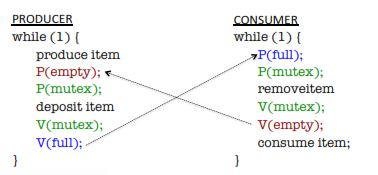
\includegraphics{img/sem_prod_cons.JPG}
\end{figure}

\paragraph{Problema dei \textit{Dining Philosophers}}
Si considerino N filosofi che spendono la loro vita a pensare e mangiare. I filosofi condividono un tavolo circolare circondato da N sedie, una per ogni filosofo. Al centro del tavolo c'è una ciotola di riso e sul tavolo sono presenti N bacchette. Quando un filosofo pensa, non interagisce con gli altri. Di tanto in tanto, un filosofo diviene affamato e cerca di prendere le due bacchette a lui più vicine. Ogni filosofo può prendere una sola bacchetta alla volta e ovviamente non può sfilarle dalle mani dei vicini. Quando un filosofo affamato ha entrambe le bacchette, può mangiare. Una volta finito, posa le bacchette e ricomincia a pensare.

Il problema dei filosofi è un classico della sincronizzazione. Una semplice soluzione è quella di rappresentare ogni bacchetta con un semaforo. Un filosofo prova a prendere una bacchetta eseguendo una \texttt{wait()} su quel semaforo, quindi la rilascia eseguendo una \texttt{signal()}. I dati condivisi sono, quindi, \texttt{semaphore chopstick[N];} , con ogni elemento inizializzato a 1.
\begin{verbatim}
do {
   wait(chopstick[i]);
   wait(chopstick[(i+1) % N]);
    . . .
   /* eat for a while */
    . . .
   signal(chopstick[i]);
   signal(chopstick[(i+1) % N]);
    . . .
   /* think for a while */
    . . .
} while(true);
\end{verbatim}

Anche se questa soluzione garantisce che due filosofi vicini non possano mangiare contemporaneamente, è incompleta perché lascia una possibilità di deadlock, qualora tutti i filosofi dovessero tentare di prendere la bacchetta alla loro destra/sinistra contemporaneamente.

Esistono svariate soluzione al problema del deadlock:
\begin{itemize}
\item Permettere a non più di N-1 filosofi di sedere al tavolo
\item Permettere a un filosofo di prendere una bacchetta solo se entrambe quelle vicino a lui sono libere
\item Usare una soluzione asimmetrica: i filosofi in un posto pari prendono per prima la bacchetta a destra, mentre quelli in un posto dispari faranno lo stesso con quella alla loro sinistra. 
\end{itemize}
Basandoci sul secondo punto, si può implementare una versione deadlock-free. Per prima cosa bisogna distinguere i tre diversi stati in cui un filosofo può trovarsi, cioè: \texttt{enum \{THINKING, HUNGRY, EATING\} state[N];}.

Il filosofo \textit{i} può settare \texttt{state[i] = EATING} solo se entrambi i suoi vicini non stanno mangiando: (\texttt{state[(i+N-1) \% N] != EATING}) and (\texttt{state[(i+1) \% N] != EATING}). 

Una soluzione corretta è quindi rappresentabile con le seguenti funzioni/classi.
\begin{figure}[htb]
  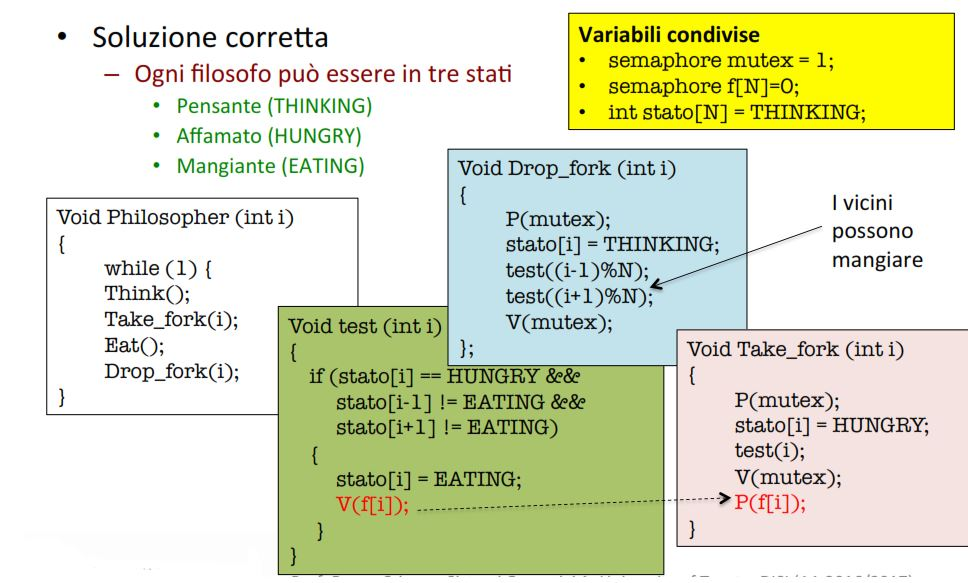
\includegraphics[width=\linewidth]{img/filosofi_ok.JPG}
\end{figure}
\newpage
\paragraph{Problema dello Sleepy Barber}
Un negozio ha una sala d'attesa con N sedie, ed una stanza con la sedia del barbiere. In assenza di clienti, il barbiere si addormenta.

Quando entra un cliente, se le sedie sono occupate, se ne va. Se il barbiere è occupato o addormentato, il cliente, rispettivamente, si siede o lo sveglia.
\begin{figure}[htb]
  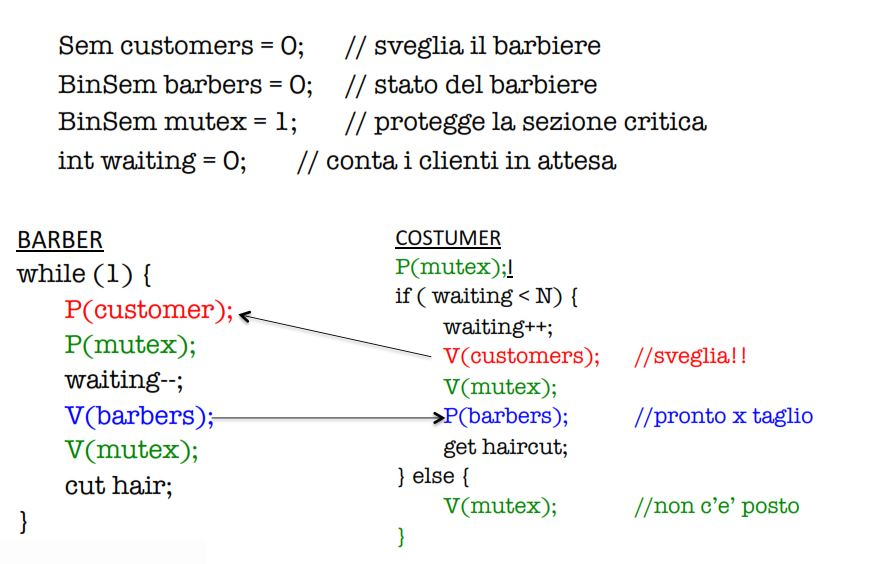
\includegraphics[width=\linewidth]{img/barber.JPG}
\end{figure}

\subsection{Monitor}
Anche se i semafori forniscono un meccanismo conveniente ed efficace per la sincronizzazione dei processi, un utilizzo sbagliato potrebbe risultare in errori sulle tempistiche difficili da scovare.

Un processo potrebbe scambiare l'ordine di esecuzione della wait() e della signal(), violando la mutua esclusione. Potrebbe addirittura rimpiazzare una signal() con una wait(), creando un deadlock. Nel peggiore dei casi potrebbe omettere una delle due chiamate, generando potenzialmente tanto un deadlock, quanto una violazione della mutua esclusione.

Per gestire tali errori, sono stati sviluppati costrutti di alto livello per la condivisione sicura ed efficiente di dati tra i processi, come, ad esempio, i monitor.

Un tipo di dato astratto (ADT -- Abstract Data Type) incapsula i dati con degli specifici set di funzioni per operarvi, indipendenti da ogni specifica implementazione del ADT. Un monitor è un ADT che include un set di procedure, fornite con mutua esclusione all'interno del monitor. Il monitor inoltre dichiara delle variabili visibili solo all'interno del monitor stesso, così come le sue procedure accedono solo alle variabili in esso definite.\newline
Il monitor assicura che un solo processo per volta sia attivo al suo interno, quindi il programmatore non deve ogni volta codificare esplicitamente la mutua esclusione.

Per permettere ad un processo di attendere all'interno del monitor, sono necessari opportuni meccanismi di sincronizzazione. Questi sono forniti dal costrutto \texttt{condition}. Si possono definire variabili del tipo \texttt{condition x,y;} all'interno del monitor. Queste saranno accessibili solo tramite due primitive interne al monitor \texttt{wait()} e \texttt{signal()}. Il processo che invoca \texttt{x.wait()} è bloccato fino all'invocazione della corrispondente \texttt{x.signal()} da parte di un altro.

Si supponga che, quando un processo P invoca \texttt{x.signal()}, ci sia un processo sospeso Q associato alla condizione x. Chiaramente, se il processo Q ha il permesso di riprendere la sua esecuzione, il processo P deve aspettare. In caso contrario, sia P che Q sarebbero attivi simultaneamente nel monitor. Esistono due possibilità:
\begin{itemize}
\item \textbf{Signal and wait.} P potrebbe aspettare finché Q non lascia il monitor o aspetta un'altra condizione
\item \textbf{Signal and continue.} Q può aspettare che P lasci il monitor o potrebbe aspettare un'altra condizione.
\end{itemize}
\paragraph{Produttore-consumatore con i monitor}
Come esempio, sfruttiamo il problema del produttore e del consumatore già precedentemente discusso. Sfruttando il monitor, la funzione che conterrà la sezione critica sarà invocata chiamando l'opportuno metodo del monitor. Perciò, il processo Producer passerà l'oggetto prodotto alla procedura enter(), mentre il consumatore rimuoverà e consumerà gli oggetti prodotti.\newline
Il monitor conterrà due variabili condizionali: full e empty, che rappresenteranno rispettivamente le code d'attesa dei processi che hanno tentato di sincronizzare le variabili condivise (gli oggetti prodotti, presenti nel buffer circolare) nel momento in cui il buffer è pieno e nel momento in cui il buffer è vuoto.
\begin{figure}[htb]
  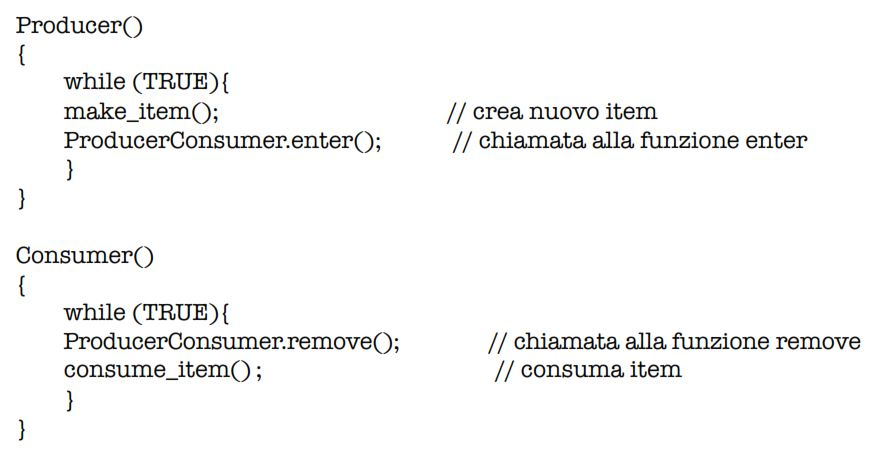
\includegraphics[width=7cm]{img/prodconsm1.JPG}
  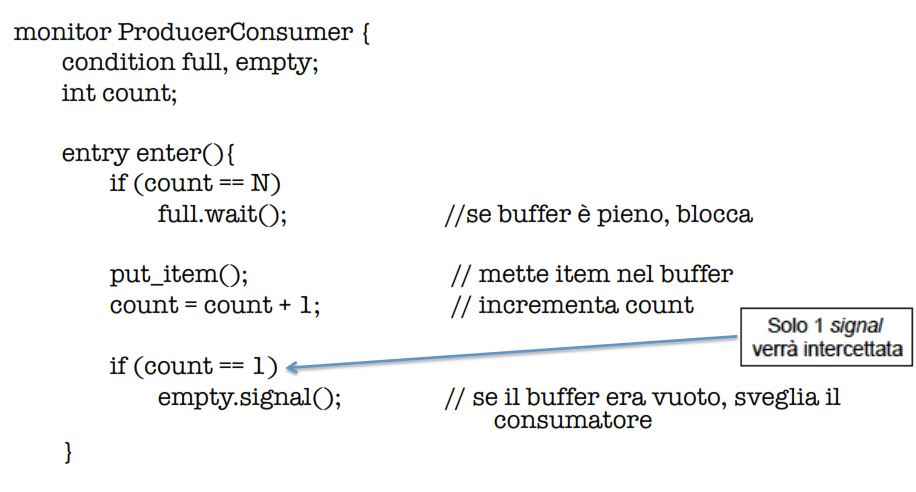
\includegraphics[width=7cm]{img/prodconsm2.JPG}
  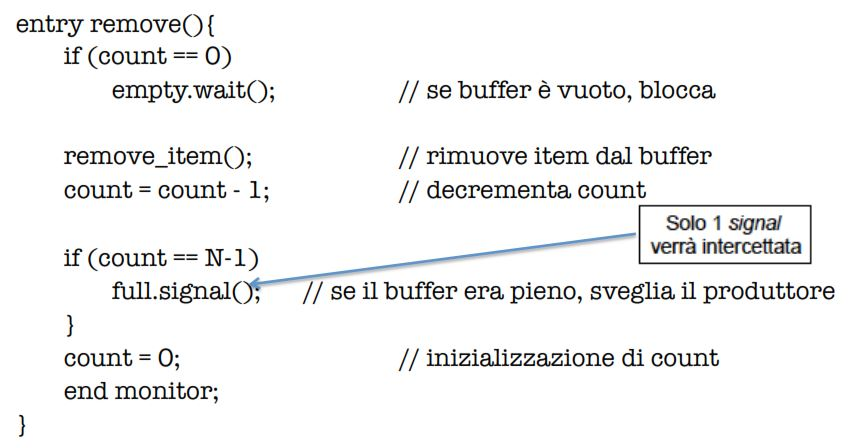
\includegraphics[width=7cm]{img/prodconsm3.JPG}
\end{figure}

\paragraph{Limitazioni}
Uno dei limiti del costrutto dei monitor è proprio la scarsa implementazione nei diversi linguaggi di programmazione. Tuttavia, si può tentare di implementarli tramite i semafori.







\newpage
\section{Deadlock}
In un sistema a multiprogrammazione, diversi processi potrebbero competere per un numero finito di risorse. Se le risorse non sono disponibili, un processo attende. A volte, un processo in attesa non riesce a cambiare stato perché sta aspettando un evento causabile solo da un altro processo, anch'esso in attesa. Questa situazione è chiamata deadlock.

\subsection{Condizioni necessarie}

Affinché si verifichi un deadlock, è necessario che le seguenti condizioni siano contemporaneamente valide in un sistema:
\begin{itemize}
\item \textbf{Mutua esclusione}: almeno una risorsa non è condivisibile, ovvero un solo processo per volta può usufruirne
\item \textbf{Hold and wait}: deve esistere un processo che detiene una risorsa e che attende di acquisirne un'altra, detenuta da un altro
\item \textbf{No preemption}: le risorse possono essere rilasciate solo volontariamente
\item \textbf{Attesa circolare}: deve esistere un insieme di processi che attendono ciclicamente il liberarsi di una risorsa
\end{itemize}
Da notare: la condizione di attesa circolare implica la Hold and Wait.

\subsection{Modello astratto (RAG)}
I deadlocks possono essere descritti in maniera più precisa utilizzando un \textit{system resource-allocation graph}, anche noto come \textbf{RAG}. Questo grafo consiste di una serie di vertici V e archi E. L'insieme V è a sua volta partizionato in nodi di tipo P (processi) e nodi di tipo R (risorse). Un arco che va da un processo a una risorsa indica che il processo richiede quella risorsa, mentre un arco che va dalla risorsa al processo indica che questo la detiene.

Data questa definizione di Grafo dell'allocazione delle risorse di sistema, è possibile dimostrare che se questo non contiene cicli, nessuno processo nel sistema si trova in uno stato di deadlock. Se invece ci sono cicli, è possibile che ci sia un deadlock, ma non sicuro. Infatti la cosa dipende dal numero di istanze per ogni risorsa: se ve ne è una sola e il grafo contiene un ciclo, si ha sicuramente un deadlock. Se invece ci sono più istanze, un ciclo non implica la presenza di un deadlock.

\subsection{Gestione dei deadlocks}
Generalmente, si può affrontare il problema dei deadlock in uno dei seguenti tre modi:
\begin{itemize}
\item Si può usare un protocollo per prevenire o evitare i deadlocks.
\item Si può permettere al sistema di entrare in uno stato di deadlock, riconoscerlo e, quindi, risolverlo
\item Si può ignorare il problema e pretendere che non possano verificarsi deadlocks nel sistema
\end{itemize}
La terza opzione è quella utilizzata dalla maggior parte dei sistemi operativi, fra cui anche Windows e Linux.\newline
Per far sì che un deadlock non si verifichi mai, il sistema può utilizzare tecniche per prevenire i deadlock, o per evitarli. La prevenzione fornisce un insieme di metodo per assicurare che almeno una delle condizioni necessarie non sia mai valida. 

La deadlock avoidance, invece, richiede che il sistema abbia informazioni addizionali su quali risorse ogni processo richiederà e userà durante la sua vita. Grazie a queste informazioni, il Sistema Operativo potrà decidere, per ogni richiesta, quanto far attendere un processo prima di soddisfarlo.

\subsection{Prevenzione dei deadlocks}
Per prevenire i deadlock è necessario impedire che si verifichi una delle quattro condizioni già citate.
\begin{enumerate}
\item \textbf{Mutua esclusione}: è irrinunciabile ed implica la presenza di almeno una risorsa non condivisibile.
\item \textbf{Hold and Wait}: per assicurare che questa condizione non si verifichi mai, è necessario garantire che, ogni volta in cui un processo richiede una risorsa, questo non ne detenga già altre, o, addirittura, abbia rilasciato tutte quelle che detiene.
Questo approccio porta a un basso utilizzo delle risorse e possibilmente alla starvation di alcuni processi, per la richiesta di risorse molto ``popolari''.
\item \textbf{No Preemption}: se un processo richiede una risorsa momentaneamente non disponibile, deve rilasciare tutte le altre risorse che detiene. In alternativa, può cedere le risorse che detiene su richiesta di un altro processo. Una soluzione simile, tuttavia, è fattibile solo per risorse il cui stato può essere facilmente ristabilito (CPU, registri... Non stampanti, nastri, ecc.)
\item \textbf{Attesa circolare}: si può assegnare una priorità (un ordinamento globale) ad ogni risorsa. Ogni processo può richiedere poi le risorse solo in ordine crescente di priorità. Così facendo, l'attesa circolare diventa impossibile perché un processo detentore di una risorsa di priorità n, prima o poi dovrà richiedere una risorsa di priorità 0 per ``chiudere il cerchio''. La priorità, e quindi l'ordine di richiesta, deve ovviamente seguire un ordine sensato (ad esempio, il disco prima della stampante).
\end{enumerate}

\subsection{Prevenzione dinamica - Deadlock Avoidance}
Le tecniche di prevenzione statica appena trattate possono portare a un basso utilizzo delle risorse poiché mettono vincoli sul modo in cui i processi possono accedere alle risorse. L'obiettivo è prevenire in base alle richieste, è quindi necessario conoscere il massimo numero di istanze di una risorsa richieste per processo. Con una tale conoscenza, il sistema può decidere, per ogni richiesta, se assegnare la risorsa al processo o farlo attendere. Per fare una tale decisione, il sistema considera le risorse attualmente disponibili, quelle attualmente allocate a ogni processo e le future richieste e rilasci dei processi.

\subsubsection{Lo Stato SAFE}
Uno stato è detto \textit{safe} se il sistema può allocare le risorse per ogni processo, in un qualche ordine, e continuare ad evitare il deadlock. L'ordine col quale le risorse vengono allocate in uno stato safe è detto \textit{sequenza safe}.

Più formalmente, una sequenza dei processi $(P_1,...,P_N)$ è safe se, per ogni $P_i$, le risorse che $P_i$ può richiedere possono essere esaudite utilizzando:
\begin{itemize}
\item le risorse disponibili
\item le risorse detenute da $P_j$, con $j < i$ (attendendo che $P_j$ termini)
\end{itemize}
Se non esiste una tale sequenza, si è in uno stato \textit{unsafe}: non tutti gli stati unsafe sono stati di deadlock, ma ne sono potenzialmente la fonte.

\paragraph{Esempio}
Si supponga di avere tre processi $P_0, P_1$ e $P_2$ e 12 istanze di una risorsa, di cui 3 libere. Le altre sono allocate nel seguente modo:
\begin{table}[htb]
\centering
\begin{tabular}{c|c|c}
     & Richieste & Possedute \\ \hline
$P_0$ & 10        & 5         \\
$P_1$ & 4         & 2         \\
$P_2$ & 9         & 2        
\end{tabular}
\end{table}
In questo caso esiste una sequenza safe $<P_1, P_0, P_2>$: $P_1$ prende le 2 risorse necessarie, quindi le rilascia. A questo punto $P_0$ potrà prendere le 5 risorse che gli mancano e completare il suo compito, quindi toccherà a $P_2$. Se $P_2$ richiedesse subito una risorsa e gli venisse assegnata, si entrerebbe in uno stato unsafe: $P_1$ potrebbe ancora eseguire, ma le 4 risorse che andrebbe poi a rilasciare non sarebbero sufficienti né per $P_0$, né per $P_2$.

L'idea è quindi quella di assicurare che il sistema rimanga sempre in uno stato safe. Inizialmente, il sistema è in uno stato safe. Ogni volta in cui un processo richiede una risorsa effettivamente disponibile, il sistema deve decidere se la risorsa può essere immediatamente allocata o no. La richiesta è soddisfatta solo se l'allocazione lascia lo stato (safe) inalterato.

Con una simile soluzione, un processo richiedente una risorsa disponibile potrebbe, dunque, essere messo in attesa. In questo modo l'utilizzo delle risorse è minore rispetto a casi in cui non si utilizzano tecniche di prevenzione dinamica. Per prevenire ciò, si possono utilizzare due soluzioni alternative: l'algoritmo con RAG o quello del banchiere.

\subsubsection{Algoritmo con RAG}
Premettendo che questo algoritmo funziona solo se si ha un'istanza per ogni risorsa, si procede così: il RAG viene ampliato con archi di reclamo, cioè vengono aggiunti degli archi, indicati con un tratteggio, da un processo a una risorsa se quest'ultima potrebbe essere richiesta in futuro dal processo. Risulta ovvio che il processo debba dichiarare tutte le risorse che chiederà ancor prima di iniziare l'esecuzione, così che queste possano apparire nel grafo. 

Quando un processo richiede effettivamente una risorsa, l'arco di reclamo diventa un arco di richiesta o, addirittura, di allocazione. Se a seguito di questa trasformazione non vengono a crearsi cicli, il sistema è in uno stato safe.

\subsubsection{Algoritmo del banchiere}
L'algoritmo con RAG non è applicabile con instanze multiple della stessa risorsa. L'algoritmo che si presenta ora è meno efficiente del RAG ma funziona con più istanze. Si chiama algoritmo del banchiere e l'idea è che la banca non deve mai \textit{distribuire tutto il denaro che ha in cassa} (=\textbf{allocare tutte le risorse}), altrimenti non potrebbe più soddisfare i bisogni dei successivi clienti.

Quando un processo entra nel sistema, deve dichiarare il massimo numero di istanze di ogni tipo di risorsa che potrebbe chiedere. Questo numero non deve eccedere il numero totale di risorse del sistema. Quando un processo richiede un set di risorse, il sistema deve determinare se l'allocare le risorse richieste lascia il sistema in uno stato safe. Per far questo c'è bisogno di un algoritmo di allocazione e di uno di verifica dello stato.

Sono necessarie diverse strutture di dati per implementare l'algoritmo del banchiere. Detti \textit{n} il numero di processi ed \textit{m} il numero di tipi di risorse, le strutture dati saranno:
\begin{itemize}
\item \textbf{available[m]}: un vettore di lunghezza m che indica il numero di risorse disponibili per ogni tipo
\item \textbf{max[n][m]}: matrice delle richieste massime di risorse 
\item \textbf{alloc[n][m]}: matrice di allocazione corrente
\item \textbf{need[n][m]}: matrice di bisogno rimanente, ovvero la differenza tra max e alloc
\end{itemize}

\paragraph{Algoritmo di allocazione}
Sia request[i][] il vettore delle richieste del processo $P_i$. Se request[i][j]==j, il processo $P_i$ vuole k istanze della risorsa $R_j$. \begin{Verbatim}[tabsize=4]
void request(int req_vec[]) {
	if (req_vec[] > need[i][])
		error(); //è stato superato il limite massimo preventivato
	if(req_vec[] > available[])
		wait //non ci sono abbastanza risorse disponibili, quindi aspetta
	//SIMULO L'ASSEGNAZIONE
	available[] = available[] - req_vec[];
	alloc[i][] = alloc[i][] + req_vec[];
	need[i][] = need[i][] - req_vec[];
	if(!state_safe()) { //Se non è safe, ripristino il vecchio stato
		available[] = available[] + req_vec[];
		alloc[i][] = alloc[i][] - req_vec[];
		need[i][] = need[i][] + req_vec[];
		wait();
	}
}
\end{Verbatim}
\newpage
\paragraph{Algoritmo di verifica dello stato}
\begin{Verbatim}[tabsize=4]
boolean state_safe(){
	int work[m] = available[]; // qui ho già sottratto le richieste di P_i
	boolean finish[n] = (FALSE,. . .,FALSE);
	int i;
	while(finish != (TRUE,...,TRUE) ) {
		//cerca P_i che NON abbia terminato e che possa completare 
		// con le risorse disponibili in work
		for(i=0; (i<n)&&(finish[i]||(need[i][]>work[])); i++);
		if (i==n) //arriva in fondo senza trovare un processo 
			    //che non abbia potenzialmente finito e un array 
			    //di risorse necessarie minore di quello delle disponibili
			return FALSE; //non c'è un arco che renda lo stato unsafe
		else {
			work[] = work[]+alloc[i][];
			finish[i] = TRUE;
		}
	} return TRUE;
}
NOTA: ritorna true e false, a un primo impatto invertiti, perché nell'algoritmo
di allocazione controlla con la negazione!
\end{Verbatim}

\paragraph{Esempio}
\begin{itemize}
\item 5 processi: P0, P1, P2, P3, P4
\item 3 risorse: A (10 istanze), B (5 istanze), C (7 istanze)
\end{itemize}
Fotografia al tempo $T_0$
\begin{table}[htb]
\centering
\begin{tabular}{c|ccc|ccc|ccc|ccc|}
\cline{2-13}
                                  & \multicolumn{3}{c|}{\textbf{Allocation}} & \multicolumn{3}{c|}{\textbf{Max}}    & \multicolumn{3}{c|}{\textbf{Available}} & \multicolumn{3}{c|}{\textbf{Need}}   \\ \cline{2-13} 
                                  & \textbf{A}   & \textbf{B}  & \textbf{C}  & \textbf{A} & \textbf{B} & \textbf{C} & \textbf{A}  & \textbf{B}  & \textbf{C}  & \textbf{A} & \textbf{B} & \textbf{C} \\ \hline
\multicolumn{1}{|c|}{\textbf{P0}} & 0            & 1           & 0           & 7          & 5          & 3          & 3           & 3           & 2           & 7          & 4          & 3          \\
\multicolumn{1}{|c|}{\textbf{P1}} & 2            & 0           & 0           & 3          & 2          & 2          &             &             &             & 1          & 2          & 2          \\
\multicolumn{1}{|c|}{\textbf{P2}} & 3            & 0           & 2           & 9          & 0          & 2          &             &             &             & 6          & 0          & 0          \\
\multicolumn{1}{|c|}{\textbf{P3}} & 2            & 1           & 1           & 2          & 2          & 2          &             &             &             & 0          & 1          & 1          \\
\multicolumn{1}{|c|}{\textbf{P4}} & 0            & 0           & 2           & 4          & 3          & 3          &             &             &             & 4          & 3          & 1          \\ \hline
\end{tabular}
\end{table}
Al tempo $T_0$ il sistema è in uno stato safe e $<P_1, P_3, P_4, P_2, P_0>$ è una sequenza safe. \newline
Al tempo $T_1$, P1 richiede (1,0,2): Request\_1 $<=$ Available? (1,0,2) $<=$ (3,3,2) ==> OK. Abbiamo quindi una nuova situazione:
\begin{figure}[htb]
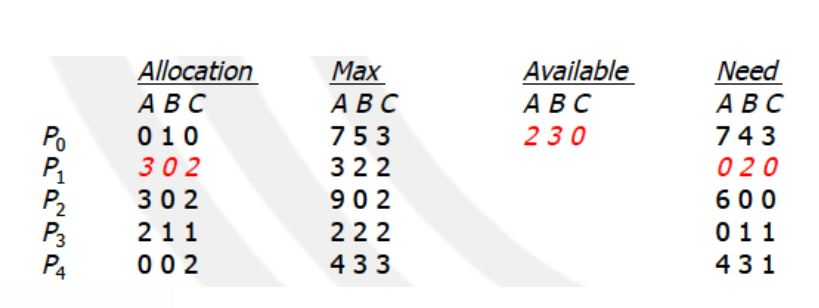
\includegraphics[width=7cm]{img/bank1.JPG}
\end{figure}
\newpage
Siamo ancora in uno stato safe?
\begin{itemize}
\item work = (2,3,0)
\item i=0 finish=FALSE, need[0] = (7,4,3) > work
\item i=1 finish=FALSE, need[1] = (0,2,0) < work
\begin{itemize}
\item work = work + (3,0,2) = (5,3,2)
\item finish[1] = TRUE
\end{itemize}
\item i=2 finish=FALSE, need[2] = (6,0,0) > work
\item i=3 finish=FALSE, need[3] = (0,1,1) < work
\begin{itemize}
\item work = work + (2,1,1) = (7,4,3)
\item finish[3] = TRUE
\end{itemize}
\item Si va avanti così e l'ordine dei finish=TRUE mi determina la sequenza safe finale, che in questo caso sarà:
\item $<P_1, P_3, P_4, P_0, P_2>$
\end{itemize}

Ad esempio, se si svolgesse l'algoritmo ipotizzando che al tempo $T_2$ P0 richiedesse (0,2,0), effettuando i dovuti cambiamenti (Allocation di P0: (0,3,0) e Available (2,1,0)), svolgendo l'algoritmo vedremmo che lo stato è unsafe.
\begin{itemize}
\item work = (2,3,0)
\item i=0 finish=FALSE, need[0] = (7,2,3) > work
\item i=1 finish=FALSE, need[1] = (0,2,0) > work
\item i=2 finish=FALSE, need[2] = (6,0,0) > work
\item i=3 finish=FALSE, need[3] = (0,3,1) > work
\item i=4 finish=FALSE, need[4] = (4,3,1) > work
\item STATO UNSAFE!
\end{itemize}

\subsection{Rilevazione del deadlock e ripristino}
Tanto la prevenzione statica quanto la dinamica sono conservative e riducono eccessivamente l'utilizzo delle risorse, quindi, al posto di algoritmi per la prevenzione o l'\textit{avoidance}, il sistema potrebbe fornire un algoritmo di rilevazione o un algoritmo di rilevazione e ripristino tramite RAG.

\paragraph{Rilevazione e ripristino con RAG}Come succedeva nella prevenzione dinamica, l'algoritmo di rilevazione e ripristino con RAG funziona solo con una risorsa per tipo. Per questo algoritmo, il grafo di allocazione delle risorse viene collassato rimuovendo i nodi delle risorse: un arco da un processo Pi a Pj implica che Pi sta aspettando che la risorsa di cui ha bisogno sia liberata da Pj. Come nel precedente caso, esiste un deadlock solo se il grafo contiene un ciclo. Per rilevare il deadlock, il sistema deve mantenere un grafo delle attese e deve periodicamente invocare un algoritmo che cerchi un ciclo nel grafo. 

\paragraph{Algoritmo di rilevazione} Il precedente algoritmo non è applicabile a sistemi con più istanze per ogni risorsa. Questo algoritmo è basato sull'esplorazione di ogni possibile sequenza di allocazione per i processi che non hanno ancora terminato. Se la sequenza va a buon fine (safe), non c'è deadlock.

Le strutture dati utilizzate sono simili a quelle dell'algoritmo del banchiere:
\begin{Verbatim}[tabsize=3]
int available[m]; //numero di istanze di R_i disponibili
int alloc[n][m]; //matrice di allocazione corrente
int req_vec[n][m]; // matrice delle richieste

int worl[m] = available[m];
bool finish[] = (FALSE,...,FALSE), found = TRUE;
while(found) {
	found=FALSE;
	for(i=0; i<n && !found; i++){
	//cerca un P_i con richiesta soddisfacibile
		if(!finish[i] && req_vec[i][]<=work[]) {
		//assume ottimisticamente che P_i esegua fino
		// al termine e che quindi restituisca le risorse
		// Se non è così, il possibile deadlock verrà
		// evidenziato alla prossima esecuzione
		// dell'algoritmo
			work[] = work[] + alloc[i][];
			finish[i]=TRUE;
			found=TRUE;
		}
	}
} //se finish[i]=FALSE per un qualsiasi i, P_i è in deadlock
\end{Verbatim}

\paragraph{Esempio}
\begin{itemize}
\item 5 processi: P0, P1, P2, P3, P4
\item 3 tipi di risorsa: A (7 istanze), B (2 istanze), C (6 istanze)
\end{itemize}
Fotografia al tempo $T_0$
\begin{figure}[htb]
  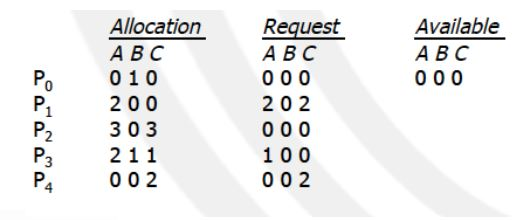
\includegraphics[width=7cm]{img/ril1.JPG}
\end{figure}
\newpage
Siamo in una situazione di deadlock?
\begin{Verbatim}[tabsize=3]
- work = (0,0,0)
- i=0	req[0] = (0,0,0) <= work 		OK
	work = work + (0,1,0) = (0,1,0)	finish[0] = true	P_0!
- i=1	req[1] = (2,0,2) <= work		NO
- i=2	req[2] = (0,0,0) <= work 		OK
	work = work + (3,0,3) = (3,1,3)	finish[2] = true	P_2!
- i=3	req[3] = (1,0,0) <= work 		OK
	work = work + (2,1,1) = (5,2,4)	finish[3] = true	P_3!
- ecc...
- La sequenza <P0, P2, P3, P1, P4> dà finish[i] = true per ogni i
\end{Verbatim}

\subsection{Utilizzo dell'algoritmo di rilevazione-ripristino}
Quanto spesso bisognerebbe chiamare l'algoritmo di rilevazione? La risposta dipende fondamentalmente dalla frequenza con cui si arriva al deadlock e quanti processi sono ogni volta coinvolti. Se i deadlock sono frequenti, l'algoritmo va invocato frequentemente.

Bisogna considerare che i deadlock capitano solo quando un processo fa una richiesta che non può essere immediatamente soddisfatta. Questa richiesta potrebbe essere proprio quella che completa una catena di processi in attesa. Nel caso estremo, quindi, si può invocare l'algoritmo di rilevazione dopo ogni richiesta non immediatamente soddisfacibile. 

Ovviamente, invocare l'algoritmo ha un peso sulle prestazioni del sistema. Un'alternativa più economica è quella di invocarlo a intervalli di tempo definiti, oppure ogni volta che l'utilizzo della CPU scende sotto una certa soglia, ricordando che un deadlock, bloccando i processi, fa eventualmente diminuire l'utilizzo di tale unità.

\subsection{Ripristino}
Quando l'algoritmo rileva un deadlock, si può agire in diversi modi.
\subsubsection{Uccisione del processi coinvolti}
Per eliminare i deadlocks terminando i processi, si possono utilizzare due approcci:
\begin{itemize}
\item Uccisione di tutti i processi. Chiaramente rompe il ciclo del deadlock, ma è molto costoso: tutti i processi devono ripartire e perdono il lavoro svolto
\item Uccisione selettiva fino alla scomparsa del deadlock. Dopo ogni uccisione bisognerà chiamare l'algoritmo, inoltre bisogna rispettare delle regole precise per la selezione del processo da uccidere di volta in volta. Queste potrebbero basarsi su priorità, tipo di risorse allocate, tempo mancante  alla fine, eccetera.
\end{itemize}

\subsubsection{Prelazione delle risorse}
Per eliminare un deadlock prelazionando le risorse, si tolgono queste in successione, di processo in processo, finché non si rompe il ciclo del deadlock.

Per prima cosa, va selezionata una vittima: come nella terminazione del processo, bisogna fare la scelta più economica. Il processo che subisce la prelazione, infatti, non potrà continuare la sua normale esecuzione.

Una volta tolta la risorsa al processo, si passa alla fase di \textbf{rollback}: bisogna far tornare il processo a uno stato sicuro e farlo ripartire da lì, dato che non può continuare la sua normale esecuzione. In genere la soluzione più semplice è un rollback totale perché, anche se più dispendiosa, questa soluzione non necessita di mantenere informazioni sullo stato del processo stesso.

Una volta prelazionata la risorsa, come ci si assicura di non andare incontro alla starvation? Bisogna assicurarsi che un processo possa essere scelto come vittima solo un numero finito (e piccolo) di volte.

\paragraph{In conclusione}, ognuno degli approcci visti ha vantaggi e svantaggi e nessuno dei tre è superiore all'altro. L'approccio basico può però essere combinato, permettendo di applicare il giusto metodo per ogni classe di risorse del sistema. Una possibile partizione in classi potrebbe essere:
\begin{enumerate}
\item Risorse interne (usate dal sistema, es: I/O)
\item Memoria
\item Risorse di processo (es. file)
\item Spazio di swap (blocchi su disco)
\end{enumerate}





\newpage
\section{Gestione della memoria}
La memoria ha un ruolo centrale nei moderni Sistemi Operativi. Essa consiste di un grande array di bytes, ognuno con il proprio indirizzo. La CPU recupera le istruzione dalla memoria in base al valore del program counter. Queste istruzioni possono causare caricamenti addizionali da e in memoria. La memoria principale e i registri del processore sono gli unici tipi di memoria accessibili direttamente dalla CPU, quindi ogni istruzione in esecuzione, ogni dato necessario, deve trovarsi lì. Se i dati non sono in quei tipi di memoria, devono esservi spostati, prima che la CPU possa utilizzarli. 

In un sistema moderno, la condivisione della memoria da parte di più processi è essenziale per l'efficienza del sistema. Per prima cosa, bisogna assicurarsi che ogni processo abbia un proprio spazio di memoria separato. Questo protegge i processi l'uno dall'altro. Per separare lo spazio di memoria, bisogna poter determinare l'intervallo degli indirizzi validi. Ciò può essere fatto utilizzando due registri, uno è detto \textbf{base register} (da dove partire), l'altro \textbf{limit register} (dimensione dell'intervallo).

Per proteggere lo spazio di memoria, la CPU confronta, con quei registri, ogni indirizzo generato in modalità utente. Ogni tentativo di eseguire un programma al di fuori dello spazio di memoria stabilito, causa una trap del sistema, meglio nota come errore fatale. 

\subsection{Binding degli indirizzi}
Per eseguire un programma, questo deve essere portato in memoria e piazzato in un processo. In base al sistema di gestione della memoria, un processo potrebbe risiedere in memoria o nel disco. I processi sul disco che stanno aspettando di essere portati in memoria formano una \textbf{input queue}. 

La normale procedura prevede il selezionare uno dei processi nella input queue e caricarlo in memoria, quindi eseguirlo. Una volta finita l'esecuzione, la memoria viene liberata. 

In molti casi, un programma utente attraversa numerose fasi, prima di essere eseguito. Gli indirizzi di memoria possono essere rappresentati in maniera diversa durante questi step. \newline
Gli indirizzi nel sorgente sono in genere simbolici (come una variabile \texttt{count}). Un compilatore, generalmente, \textit{lega (to bind)} questi indirizzi simbolici a degli indirizzi assoluti.

Il binding di dati e istruzioni a indirizzi di memoria può avvenire in tre momenti diversi:
\begin{itemize}
\item A tempo di compilazione (compile time): se è noto a priori in quale parte della memoria risiederà il processo, è possibile generare codice assoluto. Se la locazione di partenza cambia, è necessario ricompilare.
\item A tempo di caricamento (load time): se non si conosce a compile time la locazione di memoria in cui il processo risiederà, il compilatore deve generare codice rilocabile. In questo caso, il binding è ritardato fino al tempo di caricamento. Se cambia l'indirizzo di riferimento, basta ricaricare il codice.
\item A tempo di esecuzione (run time): se il proesso può essere posticipato durante la sua esecuzione da un segmento all'altro, il binding deve essere ritardato fino al run time. Per far sì che questo schema funzioni efficientemente, è richiesto un supporto hardware specifico.
\end{itemize}
Nei primi due casi si parla di binding statico, nel terzo di binding dinamico.

\subsection{Spazi di indirizzamento}
Un indirizzo generato dalla CPU è generalmente chiamato \textbf{indirizzo logico}, mentre un indirizzo visto dall'unità di memoria -- cioè, caricato nel \textbf{memory-address register} della memoria -- è comunemente chiamato \textbf{indirizzo fisico}.

Il binding degli indirizzi a compile-time e a load-time generano indirizzi logici e fisici identici, al contrario del binding a run time. Il set di tutti gli indirizzi logici generati da un programma è lo \textbf{spazio degli indirizzi logici (logical address space)}, mentre quello degli indirizzi fisici è lo spazio degli indirizzi fisici. Nel binding a run-time, il primo differisce dal secondo.

Il \textit{mapping} dall'indirizzo logico al fisico a run-time è fatto tramite un device hardware chiamato \textbf{memory-management unit (MMU)}. Il base register è ora chiamato \textbf{registro di rilocazione} e il valore che contiene va aggiunto a ogni indirizzo generato da uno processo utente, nel momento in cui questo viene mandato alla memoria. 

Il programma utente non vede mai il vero indirizzo fisico: può creare un puntatore alla locazione 346, salvarlo in memoria, manipolarlo, compararlo con altri indirizzi -- tutto con il numero 346. Solo quando è utilizzato come un indirizzo di memoria viene rilocato relativamente al registro base. In sostanza, il programma utente ha a che fare con l'indirizzo logico, mentre l'hardware di mapping della memoria lo converte nell'indirizzo fisico.

\subsection{Caricamento}
Tradizionalmente, tutto il codice deve essere caricato in memoria al tempo di esecuzione. In questo scenario, chiamato caricamento \textbf{statico}, la dimensione del processo è limitata dalla dimensione della memoria fisica. 

Per meglio utilizzare lo spazio di memoria, si ricorre al caricamento \textbf{dinamico}. In questo caso, il codice delle routines viene caricato solo quando queste vengono eseguite per la prima volta, quindi se una non dovesse mai servire, non verrebbe mai caricata in memoria, bensì resterebbe nel disco in una modalità tale da poter essere caricata appena necessaria.

\subsection{Collegamento}
Alcuno sistemi operativi supportano solo il collegamento statico, in cui le librerie di sistema e in generale tutti i riferimenti necessari al programma sono definiti prima dell'esecuzione. In particolare, l'immagine del processo, nel momento in cui andrà ad eseguire, conterrà già una copia di tutte le librerie usate.

Con il linking dinamico, il collegamento è posticipato fino al tempo di esecuzione. Il codice del programma non contiene il codice delle librerie, bensì solo un riferimento \textbf{(stub)}, cioè un piccolo pezzo di codice che indica come localizzare la routine nella libreria presente in memoria, o come caricarla (nel caso in cui non fosse già stato fatto). Lo stub viene rimpiazzato con l'indirizzo della routine e la esegue. Di conseguenza, quando quel particolare pezzo di codice dovesse essere di nuovo raggiunto, la routine di libreria verrà eseguita direttamente, senza costi aggiuntivi dati dal collegamento.

\subsection{Schemi di gestione della memoria}

\subsubsection{Allocazione contigua}
La memoria principale deve accomodare sia il sistema operativo, sia i processi utente, è pertanto necessario allocarla nella maniera più efficiente possibile.

La memoria è generalmente divisa in partizioni: quella per il sistema operativo e quella per i processi utente. Nell'allocazione contigua, ogni processo è contenuto in una sezione di memoria tale che la successiva sezione contenga il processo a lui successivo.

\paragraph{Allocazione della memoria}
Uno dei metodi più semplici per allocare la memoria è lo spezzarla in partizioni di una dimensione fissa, utilizzando quindi la \textbf{tecnica delle partizioni fisse}. In questo modo, il grado di multiprogrammazione è legato al numero di partizioni. In questo metodo, quando una partizione è libera, un processo viene selezionato dalla input queue e viene caricato nella partizione. Quando termina, la partizione viene liberata.

Nella \textbf{tecnica delle partizioni variabili}, invece, la memoria è inizialmente vista con un'immensa buca (hole) e man mano che i processi vi entrano, vanno a crearsi delle partizioni delle esatte dimensioni del processo. Man mano che i processi entreranno e se ne andranno, ovviamente, verranno a crearsi dei ``buchi'' (holes) di varie dimensioni.

In linea generale, quando un processo entra nel sistema, viene messo nella input queue. Il sistema operativo tiene conto di tutti i requisiti di memoria di ogni processo per allocargliene la giusta quantità. Quando un processo viene caricato in memoria, può competere per l'utilizzo della CPU. Quando termina, rilascia la memoria, che verrà riallocata a un altro processo nella input queue. 

In generale, come già detto la memoria è divisa in tante partizioni, di dimensione verosimilmente variabile. Quando un processo arriva e ha bisogno di memoria, il sistema deve trovare la partizione più adatta a esso, magari spezzando ulteriormente delle zone o unendone di vicine. 

In generale, si possono adottare tre approcci alla risoluzione del problema dell'allocazione della memoria:
\begin{itemize}
\item First fit. Alloca il primo hole che risulta essere grande abbastanza
\item Best fit. Alloca la più piccola buca sufficientemente grande, richiede che tutta la lista sia scandita ma garantisce il minimo spreco di memoria
\item Worst fit. Alloca la buca più grande, richiede che tutta la lista sia scansionata e lascia una buca di grandi dimensioni.
\end{itemize}

\subsubsection{Frammentazione}
Sia il first fit che il best fit soffrono di frammentazione esterna: man mano che i processi vengono caricati e rimossi dalla memoria, lo spazio viene spezzettato in pezzi sempre più piccoli.

Si parla di problema della frammentazione esterna quando c'è abbastanza memoria in totale da soddisfare una richiesta, ma gli spazi disponibili non sono contigui, risultando quindi inutilizzabili.

La frammentazione può essere anche interna, nel senso che la partizione destinata al processo è più grande di esso, quindi avrà una zona inutilizzata.

L'approccio generale per risolvere il problema della frammentazione è la compattazione: l'obiettivo è spostare il contenuto della memoria in modo che tutta quella non allocata si trovi vicina e possa essere unita in un unico, largo blocco. Ovviamente, per adottare una simile soluzione, è necessaria la rilocazione dinamica. 

\paragraph{Buddy system}
Si può trovare un compromesso tra partizioni fisse e variabili: la tecnica del buddy system. La memoria è vista come una serie di liste di blocchi di dimensione $2^K$, con L<K<U, dove $2^L$ è il più piccolo blocco allocato e $2^U$ è il più grande allocato. All'inizio tutta la memoria è disponibile come un blocco grande $2^U$. Quando arriva una richiesta, si va ad estrarre dal blocco grande $2^U$ un blocco $2^K$ adatto, ad esempio: data una memoria iniziale di 1MB e una richiesta da 100KB, la memoria risulterà partizionata in: 128K + 128K + 256K + 512K e il processo sarà piazzato in uno dei blocchi da 128 K (preferibilmente il primo).

\subsection{Segmentazione}
Si è osservato che la vista che l'utente ha della memoria non è la attuale memoria fisica. Cosa succederebbe se l'hardware potesse fornire un meccanismo di memoria che mappi il punto di vista del programmatore sulla vera memoria fisica? Il sistema avrebbe libertà nella gestione della memoria e il programmatore potrebbe muoversi in un ambiente più naturale. La segmentazione fornisce una tale meccanismo.

Un programma è in genere visto come una collezione di segmenti, cioè unità logiche che vanno a rappresentare: i vari metodi, procedure e funzioni, le variabili, lo stack, i vettori, ecc. La segmentazione fornisce proprio questa vista della memoria. Uno spazio logico degli indirizzi è una collezione di segmenti, ognuno con un nome e una dimensione. Gli indirizzi specificano sia il nome del segmento che l'offset al suo interno. Il programmatore specifica perciò ogni indirizzo con la tupla <numero di segmento, offset>. 

Il mapping dall'indirizzo bidimensionale del programmatore a quello fisico viene fatto tramite una tabella dei segmenti (segment table). Ogni entry della tabella contiene una base, cioè l'indirizzo fisico di partenza del segmento in memoria e un limite, cioè la lunghezza del segmento. Un indirizzo logico consiste di due parti: un numero di segmento s e un offset d. Quando un offset è legale, cioè è minore del limite, viene aggiunto alla base del segmento per produrre l'indirizzo del byte desiderato nella memoria fisica. 

Ad esempio, si consideri la seguente situazione:
\begin{figure}[htb]
  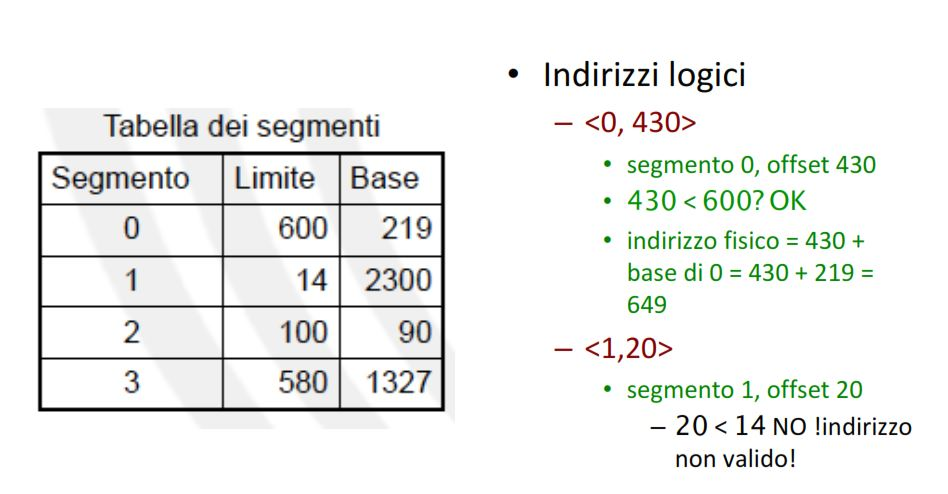
\includegraphics[width=12cm]{img/segmem.JPG}
\end{figure}

\subsection{Paginazione}
La paginazione, come la segmentazione, permette di avere uno spazio fisico degli indirizzi di un processo \textit{non contiguo}. In aggiunta a questo, la pagina elimina la frammentazione esterna e la necessità di compattazione. 

Il metodo di base per l'implementazione della paginazione prevede di ``rompere'' la memoria fisica in blocchi di grandezza fissata chiamati \textbf{frames}, mentre la memoria logica viene spezzata in blocchi della stessa dimensione, chiamati \textbf{pagine}.

Risulterà a questo punto ovvio che un programma avente dimensione \textit n pagine, potrà essere eseguito solo trovando \textit n frames liberi.

Ogni indirizzo generato dalla CPU si compone di due parti: un numero di pagina (p) e un offset (d). Il numero di pagina è utilizzato come indice in una tabella delle pagine (page table). La tabella contiene l'indirizzo base di ogni pagina nella memoria fisica. Questo indirizzo di base è combinato con l'offset per definire l'indirizzo fisico di memoria.

La dimensione della pagina (e del frame) è definita dall'hardware ed è sempre una potenza di 2. Questo permette una facile traduzione degli indirizzi. Se la dimensione dello spazio logico degli indirizzi è $2^m$ e una pagina è grande $2^n$, i primi $m-n$ bit di un indirizzo saranno il numero di pagina p e i restanti n bit saranno l'offset. Ad esempio, con una memoria da 8KB e pagine da 1KB, l'indirizzo logico 936 diventa l'indirizzo fisico 1960 (pagina 0 su frame 1 (1024...2047), offset=936, indirizzo fisico = 1024+936=1960).

Si potrà notare che questo sistema elimina la frammentazione esterna, mentre permane quella interna. In media, infatti, mezza pagina per processo verrà sprecata, è quindi preferibile lavorare con pagine non troppo grandi. 

\subsubsection{Implementazione della tabella delle pagine}
Ogni sistema operativo ha il proprio metodo per mantenere le tabelle delle pagine e l'implementazione hardware può essere fatta in molti modi diversi. Nel caso più semplice, la tabella è implementata come un set di registri dedicati, costruiti con una logica che permetta l'efficienza maggiore possibile: ogni accesso alla memoria deve superare il mapping delle pagine, quindi è molto importante che possa essere fatto velocemente, soprattutto perché ogni volta è necessario un context switch per salvare i registri.

L'uso dei registri è soddisfacente se la tabella è sufficientemente piccola, dato il limitato numero di tali dispositivi, ma al giorno d'oggi i computer supportano tabelle molto vaste. Per venire incontro a questa esigenza, è preferibile tenere la tabella delle pagine in memoria e usare uno o al più due registri: il page-table base register (PTBR), che contiene un puntatore alla tabella, e il page-table lenght register (PTLR), che è opzionale e contiene la dimensione della tabella. In questo modo, il context switch è molto più breve perché richiede solo la modifica del PTBR e, al massimo, del PTLR.

\begin{wrapfigure}{r}{5.5cm}
  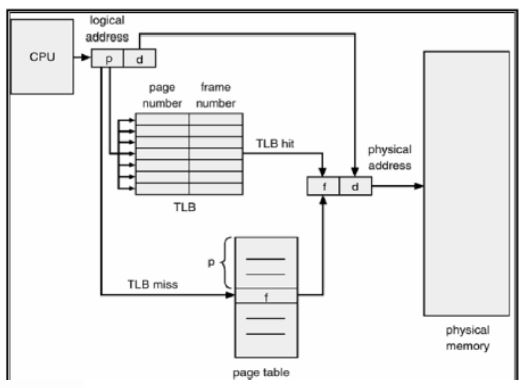
\includegraphics[width=7cm]{img/tlb.JPG}
\end{wrapfigure}
Il problema con questo approccio è che richiede due accessi in memoria: uno per andare a leggere la tabella e uno per andare alla voce indicata, quindi il tempo di accesso alla memoria è moltiplicato da un fattore 2. Per risolvere tale problema, si può utilizzare una piccola cache veloce detta translation look-aside buffer (TLB). Ogni entry nel TLB consiste di due parti: una chiave e un valore.  Quando gli viene presentato un oggetto, questo viene comparato con tutte le chiavi simultaneamente. Se viene trovato, viene ritornato il valore corrispondente. 
Il meccanismo del TLB è molto costoso, per questo al suo interno viene memorizzato solo un piccolo sottoinsieme delle entry nella tabella delle pagine e ad ogni context switch viene ripulito per evitare il mapping di indirizzi errati.

Durante un accesso alla memoria, se la pagina cercata è nel TLB, questo restituisce il numero di frame con un singolo accesso. In caso contrario, è necessario accedere alla tabella delle pagine in memoria.

La percentuale di volte in cui una pagina di interesse si trova nel TLB è detta hit ratio. Se non si trova la pagina in TLB, bisogna accedere alla memoria per andare alla tabella delle pagine e recuperare il numero di frame, quindi bisogna riaccedere in memoria al frame appena indicato. Ipotizzando che l'hit ratio sia dell'80\% e ogni accesso in memoria richieda 100ns, il \textbf{tempo di accesso effettivo} sarà calcolato come: \newline
$ effective\_access\_time = \alpha * (T_{TLB}+T_{mem}) + (1-\alpha) * (T_{TLB}+T_{mem} + T_{mem}) $\newline
cioè, nel nostro caso, supponendo $T_{TLB} = 10ns$, si ha:\newline
$ eat = 0.80 * 110ns + 0.20 * 210ns = 130ns $\newline

\subsubsection{Protezione}
La protezione è realizzata associando un bit di protezione ad ogni frame. Normalmente, questi bit sono mantenuti nella tabella delle pagine.
\paragraph{Bit di accesso} Un bit può essere utilizzato per definire se una pagina è di lettura-scrittura o di sola-lettura. Questo bit può essere controllato ogni volta che si accede alla pagina per controllare che non si scriva su una pagina in cui la scrittura non è abilitata (causando una trap).
\paragraph{Bit di validità} Un bit aggiuntivo è allegato a ogni entry della tabella delle pagine. Quando questo bit è settato a \textit{valid}, la pagina associata è nello spazio di indirizzamento logico del processo, mentre se è settato a \textit{invalid}, la pagina non si trova nello spazio di indirizzamento logico del processo. Un tentativo di accesso a una tale pagina causa una trap del sistema. Il bit di validità potrebbe non bastare, soprattutto nel caso in cui una pagina non fosse interamente utilizzata. Ad esempio, in un processo che occupa 3 pagine e mezza, la quarta sarà segnata come valida. Il precedentemente citato PTLR serve come ulteriore sicurezza per evitare che il processo possa accedere alla metà della quarta pagina fuori dal suo range.

\begin{wrapfigure}{r}{5.5cm}
  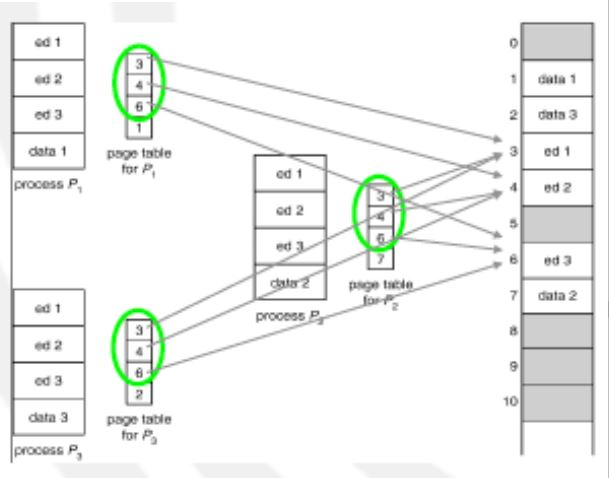
\includegraphics[width=9cm]{img/pag_cond.JPG}
\end{wrapfigure}
\subsubsection{Pagine condivise}
Uno dei vantaggi dell'uso della paginazione è la possibilità di condividere codice (a patto che non cambi durante la sua esecuzione). Così facendo, una sola copia del codice deve essere tenuta in memoria fisica, mentre poi ogni processo avrà la propria copia logica, con i propri dati. Il vantaggio è che se 40 utenti vogliono utilizzare contemporaneamente un editor, il cui ``peso'' è di 150KB, più 50KB per lo spazio dati di ogni utente, non ci sarà bisogno di fare 40 copie di editor e spazio dati (totale 40 * 200KB), bensì serviranno solo 40 copie dello spazio dati, mentre il codice dell'editor sarà accessibile da tutti (150 + 40*50).

\subsection{Struttura della Tabella delle Pagine}
Nelle architetture moderne con 32 o 64 bit di indirizzo, lo spazio di indirizzamento virtuale è pari a $2^32$ o $2^64$, ovvero molto maggiore dello spazio fisico. In un tale ambiente, la tabella delle pagine diventa eccessivamente grande. Si consideri, ad esempio, un sistema a 32 bit. Se in tale sistema una pagina è da 4KB ($2^12$), una tabella delle pagine potrebbe avere un milione di entry ($2^32 / 2^12$) per ogni processo. Se si considera che ogni entry abbia una dimensione di 4 bytes, ogni processo avrà bisogno di 4MB di spazio solo per la page table. Chiaramente, non si vuole allocare una tale tabella in maniera contigua in memoria.

La soluzione più semplice sta nel dividere la tabella in pezzi più piccoli.

\begin{wrapfigure}{r}{5.5cm}
  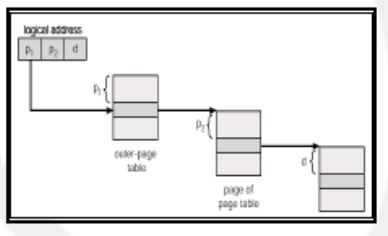
\includegraphics[width=7cm]{img/pagpag.JPG}
\end{wrapfigure}
\subsubsection{Paginazione multilivello}
Questo metodo consiste nel ``paginare'' la tabella delle pagine. In pratica, solo alcune parti della tabella delle pagine sono memorizzate esplicitamente in memoria, mentre le altre sono su dischi. In generale, un indirizzo logico ha dei bit che indicato il numero di pagina e altri che indicano l'offset. Paginando la tabella delle pagine, la parte del numero di pagina verrà ulteriormente divisa in una parte che indicherà la tabella ``esterna'' e una che indica l'offset all'interno della tabella ``interna''.
Ad esempio, dato un indirizzo: \newline
\begin{table}[htb]
\centering
\begin{tabular}{ccc}
p1                               & p2                              & offset                            \\ \hline
\multicolumn{1}{|c|}{0000000001} & \multicolumn{1}{c|}{0000000011} & \multicolumn{1}{c|}{000000000100} \\ \hline
\end{tabular}
\end{table} \newline
Si avrà:
\begin{itemize}
\item p1=1 : recuperare la tabella di livello 2 corrispondente all'indirizzo indicato dalla prima riga
\item p2=3 : recuperare l'indirizzo indicato nella teza riga della tabella di livello 2
\item offset=4 : da sommare al valore fornito nella terza riga della tabella di livello 2
\end{itemize}
Così facendo, ogni livello è memorizzato come una tabella separata in memoria, quindi la conversione dell'indirizzo logico in quello fisico può richiedere n+1 accessi in memoria, per una paginazione di n livelli. Tuttavia, il TLB mantiene le prestazioni a livelli ragionevoli.

\subsubsection{Tabelle delle pagine di tipo hash}
Un'alternativa alla paginazione a più livelli utilizzata in alcune architetture a 32 bit, cosiste nell'usare Page Tables in cui le varie pagine sono raggruppate secondo una funzione di hashing.

\subsubsection{Tabella delle pagine invertita}
Solitamente, ogni processo ha una page table associata. Considerando che ogni page table può avere svariate centinaia o migliaia di entries, una tale soluzione consuma troppa memoria.

Per risolvere questo problema si può utilizzare una tabella delle pagine invertita. In questo modo, c'è un'unica tabella per nel sistema, la quale ha una entry per ogni frame (pagina fisica), contenente la coppia <process-id, page-number>, dove process-id è l'identificativo del processo che possiede la pagina e page-number è l'indirizzo logico della pagina contenuta nel frame corrispondente alla entry. 

Ogni indirizzo logico generato dalla CPU è una tripla <process-id, page-number, offset>. Quando viene fatto un riferimento a una zona di memoria, le prime due parti dell'indirizzo richiesto sono presentate al ``sottosistema'' si memoria. Se si ha una corrispondenza, viene generato l'indirizzo fisico <entry-i, offset>. Se l'indirizzo non viene trovato, si ha un trap del sistema.

Anche se questo schema diminuisce la quantità di memoria necessaria a mantenere ogni tabella delle pagine, aumenta il tempo necessario per cercare un riferimento a una pagina. Infatti, poiché la tabella delle pagine invertita è ordinata secondo gli indirizzi fisici, ma il lookup viene fatto secondo quelli virtuali, potrebbe essere necessario scorrerla tutta ogni volta. Per risolvere questo problema, si può usare l'equivalente di una hashtable, così che il tempo di ricerca si riduca da O(n) a O(1). Ovviamente, ogni accesso alla hashtable aggiunge un riferimento alla memoria, quindi per mappare un indirizzo logico servono almeno due letture in memoria, una per la hash table e una per la page table.

I sistemi che utilizzano la tabella invertita hanno difficoltà ad implementare un sistema di condivisione delle pagine perché avrebbero bisogno di mappare uno stesso indirizzo fisico su più indirizzi logici (virtuali). Risulta quindi necessario un meccanismo per gestire le collisioni quando diversi indirizzi virtuali corrispondono allo stesso frame (per capire se è un frame condiviso o no).







\newpage
\section{Memoria Virtuale}
Le tecniche viste finora prevedono che un processo, per essere eseguito, debba risiedere interamente in memoria. L'utilizzo della memoria virtuale permette l'esecuzione di processi che non sono completamente in memoria, permettendo quindi l'utilizzo di programmi più grandi della memoria fisica. Inoltre, la memoria virtuale astrae la memoria fisica in un array uniforme estremamente vasto, separando la memoria logica (vista dall'utente) da quella fisica. 

La memoria virtuale facilita inoltre la condivisione di files e di memoria tra i processi e fornisce un meccanismo efficiente per la loro creazione. 

Tuttavia, la memoria virtuale non è di facile implementazione e può danneggiare le prestazioni se utilizzata in maniera inappropriata.

\begin{wrapfigure}{r}{5.5cm}
  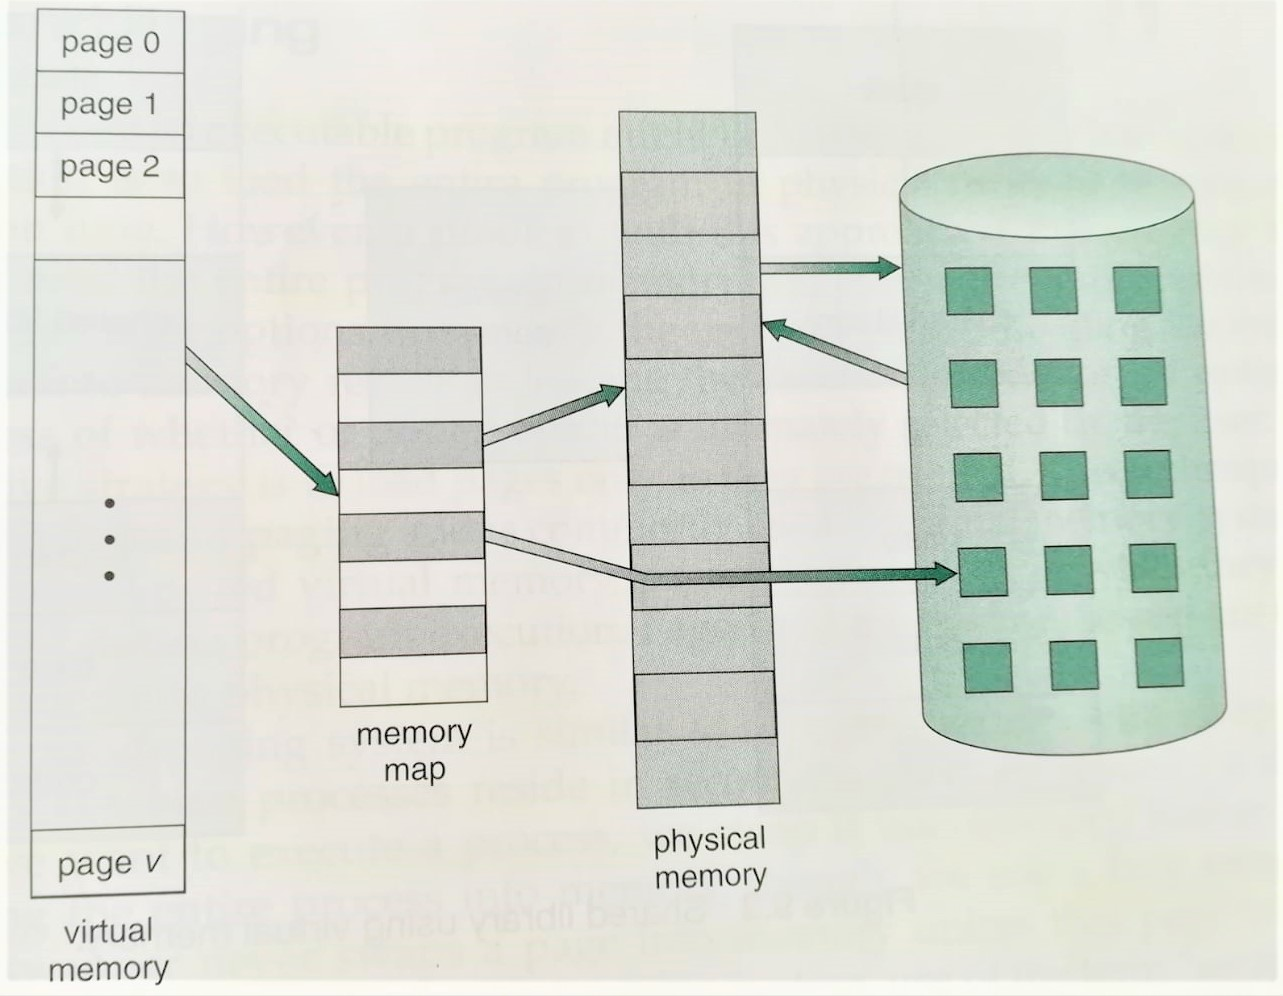
\includegraphics[width=7cm]{img/virtmem.jpeg}
\end{wrapfigure}
Il concetto chiave è nella possibilità di swappare pagine -- e non l'intero processo -- da e verso la memoria. La memoria virtuale è quindi composta dalla memoria fisica e dal disco. 

Lo spazio di indirizzamento virtuale di un processo si riferisce alla vista logica (o virtuale) di come un processo è mantenuto in memoria. 

Esistono due metodi principali per l'implementazione della memoria virtuale: la paginazione su domanda (demad paging) e la segmentazione su domanda (demand segmentation).

\subsection{Paginazione su domanda}
Si consideri come un programma eseguibile può essere caricato dal disco alla memoria. Un'opzione è quella di caricare tutto il programma nella memoria fisica a tempo di esecuzione. Tuttavia, si potrebbe non aver bisogno dell'intero programma in memoria fin da subito; la cosa risulterebbe in uno spreco di spazio. Una strategia alternativa è quella di caricare le pagine solo se necessarie. 

\begin{wrapfigure}{r}{5.5cm}
  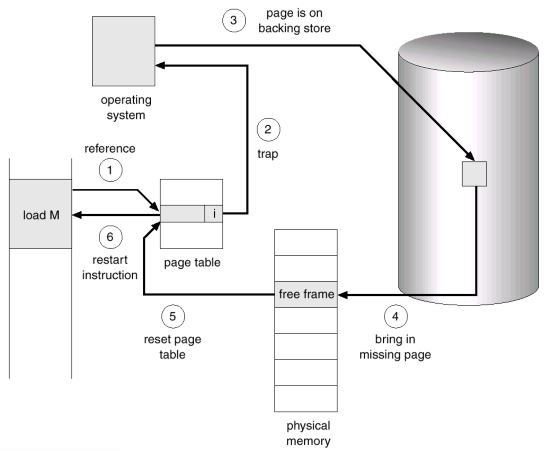
\includegraphics[width=7cm]{img/pagefault.JPG}
\end{wrapfigure}

Con la memoria virtuale implementata tramite paginazione su domanda, le pagine sono caricate solo quando sono richieste durante l'esecuzione. Delle pagine che non sono mai richieste, magari con codice per casi particolari, non vengono mai caricate in memoria.

 Quando un processo viene swappato in memoria, è necessario ``indovinare'' quali pagine dovranno essere utilizzate prima che il processo venga swappato di nuovo fuori dalla memoria. C'è quindi la necessità di un supporto hardware per distinguere tra le pagine che sono in memoria e le pagine che sono nel disco. Il bit di validità può essere utile in questo caso: quando è \textit{valid} la pagina è valida e in memoria, quando è \textit{invalid} la pagina è o non valida o valida ma sul disco. Se all'inizio vengono caricate le pagine ``giuste'', il processo eseguirà esattamente come se fossero state caricate tutte le pagine in memoria. 

Cosa succede se un processo prova ad accedere a una pagina non caricata in memoria? L'accesso a una pagina invalida causa un \textbf{page fault}. L'hardware per la paginazione, nel tradurre l'indirizzo attraverso la tabella delle pagine, noterà che il bit di validità è settato su \textit{invalid} e causerà una trap del sistema operativo. La procedura per gestire i pagefault è la seguente:

\begin{itemize}
\item Il Sistema Operativo verifica una tabella (associata al processo) per determinare se il riferimento alla pagina è valido o no.
\item Se il riferimento era invalid, il processo viene terminato. Se era valido e la pagina non era ancora stata caricata in memoria, se ne attiva il caricamento
\item Viene cercato un frame libero
\item Si swappa la pagina dal disco nel frame
\item Quando la lettura dal disco è completata, viene modificata la tabella interna del processo e la tabella delle pagine per indicare che una pagina è ora in memoria.
\item L'istruzione che aveva causato il page fault viene rispristinata.
\end{itemize} 
In un caso estremo, si può iniziare ad eseguire un processo con nessuna pagina in memoria, dando luogo ad un page fault già al primo accesso in memoria. Con questa modalità si ha demand paging puro: non si porta mai una pagina in memoria finché non è esplicitamente richiesta.

\paragraph{Performance}
La paginazione su domande influenza il tempo di accesso effettiva alla memoria. Sia \textit p la probabilità che avvenga un page fault e \textit{ma} il tempo di accesso alla memoria:
$ EAT = (1-p) * ma + p * t_{pageFault} $
$ t_{pageFault} $ è dato da tre componenti principali: il servizio dell'interrupt, lo swap-in (lettura della pagina) e out (opzionale) e il costo del riavvio del processo. Il valore in genere è molto maggiore del tempo di accesso alla memoria (si parla di ordini di grandezza di differenza), è quindi fondamentale riuscire a mantenere un tasso di page fault basso.

\subsubsection{Rimpiazzamento delle pagine}
Cosa succede se non ci sono frames liberi in memoria per caricare le pagine? Il Sistema Operativo ha molte opzioni per procedere. Potrebbe terminare il processo, ma va contro il principio della trasparenza all'utente (che non deve accorgersi della cosa). Potrebbe altrimenti fare uno swap-out di un processo, liberando tutti i frames a esso allocati e riducendo il grado di multiprogrammazione. Può altrimenti procedere con il \textbf{rimpiazzamento delle pagine}.

Con questo metodo, se nessun frame è libero, se ne cerca uno momentaneamente inutilizzato e lo si libera, cioè il suo contenuto viene messo nello spazio di swap e la tabella delle pagine viene cambiata per indicare che quella pagina non è più in memoria. La gestione dei page fault in assenza di frames liberi è, quindi, la seguente:
\begin{itemize}
\item Il Sistema Operativo verifica una tabella (associata al processo) per capire se si tratta di page fault o violazione di accesso
\item Cerca un frame vuoto
\begin{itemize}
\item Se esiste, OK.
\item Se non c'è, si usa un algoritmo di rimpiazzamento delle pagine per scelgiere un frame vittima
\end{itemize}
\item Swap della vittima su disco
\item Swap della pagina dal disco al frame
\item Modifica delle tabelle
\item Ripristino dell'istruzione che ha causato il page fault
\end{itemize}
Si noti che, se non ci sono frames liberi, è necessario swappare due pagine, andando quindi a raddoppiare il tempo di page fault ed aumentando di conseguenza il tempo di accesso effettivo alla memoria (EAT).
Si può ottimizzare il meccanismo utilizzando un bti di modifica (modify bit o dirty bit). Ogni pagina ha questo bit associato ed è settato a 1 se la pagina è stata modificata (scrittura) dal momento del suo accesso in memoria. Solo le pagine che risultano modificate (bit=1) vengono scritte su disco quando sono scelte come vittime. Non è necessario scrivere su disco una pagina con bit=0 perché, ovviamente, non ha ancora subito modifiche da salvare.

Questo schema può ridurre significativamente il tempo richiesto per affrontare un page fault, dato che dimezza il tempo di I/O se la pagina non è stata ancora modificata. 

\subsubsection{Algoritmi di rimpiazzamento delle pagine}
Il rimpiazzamento delle pagine è fondamentale alla paginazione su domanda, ma bisogna risolvere due grandi problemi per la completa implementazione: bisogna sviluppare un algoritmo di allocazione dei frames e un algoritmo di rimpiazzamento delle pagine. Vale a dire, se si hanno più processi in memoria, bisogna decidere quanti frame vanno allocati ad ogni processo e, quando viene richiesto di rimpiazzare una pagina, quale frame scegliere come vittima.

La valutazione per la scelta dell'algoritmo viene effettuata facendolo eseguire su una particolare stringa di riferimenti alla memoria e calcolando il numero di page fault, il cui tasso deve essere tenuto al minimo possibile. La stringa citata è detta \textbf{reference string}. Data la dimensione p di una pagina, si deve considerare solo il numero di pagina e non l'intero indirizzo. Ergo, dati i seguenti ``indirizzi'':

0100, 0432, 0101, 0612, 0102, 0103, 0101, 0611

Considerando pagine di 100 bytes, la sequenza si riduce alla seguente stringa (è inutile specificare riferimenti multipli e sequenziali alla stessa pagina):

1, 4, 1, 6, 1, 6

\paragraph{Algoritmo FIFO}
Nel più semplice degli algoritmi, la prima pagina introdotta è la prima ad essere rimossa.

L'algoritmo è ``cieco'', vale a dire che non viene valutata l'importanza della pagina rimossa, quindi la rimozione di una pagina cui si fa spesso riferimento, potrebbe portare a un significativo incremento del tasso di page-fault. L'algoritmo è inoltre soggetto all'anomalia di Belady: il tasso di page-fault può aumentare all'aumentare dei frame associati (in determinati casi).

\paragraph{Algoritmo ideale}
Garantisce il minimo numero di page fault, andando a rimpiazzare la pagina che non verrà usata per il più lungo periodo di tempo.

La difficoltà nell'implementazione di questo algoritmo risiede nella necessità di conoscere in anticipo la reference string (si incontra un problema simile con l'algoritmo di scheduling SJF). Essendo impossibile da implementare, viene usato per lo più come riferimento per gli altri algoritmi.

\paragraph{Algoritmo Least Recently Used (LRU)} È un'approssimazione dell'algoritmo ottimale. FIFO utilizza il tempo in cui una pagina è stata portata in memoria, l'ideale utilizza il tempo in cui essa vi rimarrà. LRU utilizza il passato recente per prevedere il futuro e va a rimpiazzare la pagina che non viene usata da più tempo. L'algoritmo è migliore del FIFO ed ovviamente peggiore dell'ideale.

L'implementazione non è banale, in quanto bisogna comunque ricavare il tempo dell'ultimo utilizzo e può richiedere notevole hardware addizionale.

Una possibile implementazione è tramite \textbf{contatore}: ad ogni pagina è associato un contatore in cui viene copiato il clock di sistema ogni volta che la pagina viene referenziata. La pagina da rimpiazzare sarà quella con il più piccolo valore del contatore. 

Una seconda implementazione sfrutto lo \textbf{stack}: se ne mantiene uno con i numeri di pagina. Ad ogni riferimento ad una pagina, questa viene messa in cima allo stack e quella in fondo sarà la vittima scelta da LRU. Ogni update dello stack è un po' più costoso della copia del clock di sistema nel counter, ma tale costo si recupera considerando che non c'è bisogno di un algoritmo di ricerca.

Molti sistemi, altrimenti, utilizzano un \textbf{bit di reference}: associato ad ogni pagina, inizialmente è settato a 0. Quando la pagina viene referenziata, viene messo a 1 e per il rimpiazzamento si sceglie una pagina che ha il bit a 0. Così facendo, l'algoritmo è solo approssimato poiché non si considera un ordine di riferimento delle pagine.

In alternativa, si può tenere una \textbf{sequenza di 8 bit} per ogni pagina. A intervalli regolari, il sistema operativo shifta i bit verso destra. Questi 8 bit contengono uno storico dell'utilizzo della pagina: un bit a 1 significa che in quell'intervallo di tempo la pagina è stata usata, 0 altrimenti. Il byte viene interpretato come un intero unsigned e la pagina vittima sarà quella con il valore più basso.

Altre tecniche sono basate sul conteggio. L'algoritmo LFU (Least Frequently Used) mantiene un conteggio del numero di riferimenti fatti ad ogni pagina e va a rimpiazzare quella con il valore più basso. Questa pagina potrebbe non corrispondere a quella selezionata con LRU. L'algoritmo MFU, al contrario, scarta quella col valore più alto.

Un'ulteriore soluzione si chiama \textbf{rimpiazzamento second chance}. L'algoritmo si basa su una coda FIFO circolare e sull'utilizzo del bit di reference. Quando una pagina viene selezionata, si controlla il bit di reference: se è 0, la si rimpiazza, se è 1, si setta il bit a 0 e la si lascia in memoria (seconda possibilità), quindi si va avanti nella coda.

\subsubsection{Allocazione dei frame}
 Data una memoria con N frame ed M processi, è importante scegliere bene quanti frame allocare per ogni processo. Questo numero è soggetto a dei vincoli: ogni processo necessia di un minimo numero di pagine per poter eseguito e questo minimo è dettato dal fatto che l'istruzione interrotta da un page fault deve essere rieseguita. Di conseguenza, il minimo numero di pagine è il massimo numero di indirizzi specificabile in una istruzione.
 
 Il modo più facile di dividere N frame tra M processi è quello di dare ad ognuno N/M frames. Questo schema è chiamato \textbf{equal allocation}. Si può altrimenti utilizzare l'allocazione proporzionale, in cui si alloca un numero di frames proporzionare alla dimensione del processo. In questo caso bisogna considerare che la priorità potrebbe essere comunque più significativa della sua dimensione.
 
 Un altro aspetto da considerare è il modo in cui si svolge il textbf{rimpiazzamento delle pagine}. Secondo il global replacement, un processo può selezionare un frame vittima dall'intero set dei frames, anche se al momento è allocato a un altro processo. Con il local replacement, al contrario, può rimpiazzare solo un fram appartenente al set per lui allocato.
 
 Esistono inoltre due schemi di allocazione dei frames. L'allocazione fissa prevede che ad un processo sia attribuito sempre lo stesso numero di frames, mentre l'allocazione variabile prevedere che il numero possa variare durante l'esecuzione. Il problema ora è: in base a cosa modifico questo numero? La scelta può essere fatta sulla base del calcolo del working set o sul calcolo del page fault frequency (PFF).
 
 \paragraph{Calcolo del working set}
 Un criterio per rimodulare l'allocazione dei frame consiste nel calcolare in qualche modo quali sono le richieste effettive di ogni processo. Questo viene fatto in base al modello della località, che prevede che un processo, durante la sua esecuzione, passi da una località (din indirizzi) all'altra. Una località è un set di pagine usate attivamente insieme. Idealmente, un processo necessita di un numero di frame pari alla sua località. Per calcolarla, si prende in analisi un intervallo dei riferimenti in memoria più recenti, cioè il working-set. Se una pagina è attivamente in uso, si troverà nel working set. Il numero di pagine nel working set deve essere ragionevole: se è troppo piccolo, è poco significativo, mentre se è troppo grande, può coprire anche altre località. Una volta selezionata la dimensione della finestra del working-set, il suo utilizzo è semplice. Il sistema operativo monitora il working-set di ogni processo e gli alloca un numero sufficiente di frames. Se ci sono abbastanza frames di avanzo, può inizializzare un nuovo processo. Se la somma dei vari working-sets va a superare il numero di frames disponibili totali, il sistema seleziona un processo da sospendere.
 
 Il valore del working set può essere approssimato tramite timer e bit di reference. Si può far uso di un timer che interrompe periodicamente la CPU e all'inizio di ogni periodo si pone a 0 il bit. Ad ogni interruzione si scandiscono le pagine: quelle a 1 sono nel working set e quelle a 0 vengono scartate. 
 
 \paragraph{Thrashing} Quando il numero totale dei frames richiesti supera quello dei frames totali, si verifica un fenomeno noto come thrashing: un processo spende tempo di CPU continuando a swappare pagine da e verso la memoria, l'utilizzo della CPU va quindi a diminuire. Questo viene interpretato dal sistema operativo come un segnale per aumentare la multiprogrammazione, ma questo fa aumentare ancora di più il tasso di page fault e si entra in un circolo vizioso. 
 
 \paragraph{Frequenza dei page fault}
 Il problema specifico è prevenire il thrashing, cioè un alto tasso di page fault. Si vuole quindi controllare questo tasso. Si sa che se questo è troppo alto, il processo ha bisogno di più frames, mentre se è troppo basso ne ha troppi e li rilascia.
 
 \subsubsection{Considerazioni generali}
 Il thrashing e il risultante swapping hanno un grosso impatto sulle prestazioni. La miglior pratica per contrastare questo problema, al momento, è quella di includere una quantità adatta di memoria fisica nel proprio computer.
 
 Un altro tassello importante è la selezione della dimensione della pagina, ricordando che le pagine piccole portano a frammentazione esterna e pagine grandi a quella interna. La dimensione della tabella delle pagine è inversamente proporzionale alla dimensione delle pagine. L'overhead di I/O è meglio ammortizzato per le pagine grandi, mentre per la località sono migliori le piccole, poiché consentono di avere un ``maggior dettaglio''.
 
 La stessa struttura di un programma influisce sul numero di page fault. Ad esempio, dato un array A[1024][1024] di interi, in cui ogni riga è memorizzata in una pagina, se si scrive:
\begin{Verbatim}
for j:= 1 to 1024 do
	for i := 1 to 1024 do
		A[i][j] := 0;
\end{Verbatim}
si avranno 1024*1024 page fault, mentre scrivendo:
\begin{Verbatim}
for i:= 1 to 1024 do
	for j := 1 to 1024 do
		A[i][j] := 0;
\end{Verbatim} 
si avranno solo 1024 page fault.

Infine, bisogna anche considerare che potrebbero esserci alcuni frame bloccati, cioè frames che non devono mai essere rimpiazzati, quali quelli corrispondenti a pagine del kernel o a pagine utilizzate per trasferire dati da e verso l'I/O.






\newpage
\section{Gestione della memoria secondaria}

\subsection{Tipologie del supporto}
In questa sezione, si tratta in maniera generale la struttura fisica dei device utilizzati come memoria secondaria.

\paragraph{Nastri magnetici}
Non sono altro che una sottile striscia in materiale plastico, rivestita di un materiale magnetizzabile. Sono stati usati per memorizzare dati digitali per la prima volta nel 1951. Hanno una capienza massima di circa 5TB (dato del 2011) e sono gestiti con accesso sequenziale. Hanno una velocità molto inferiore a quella della memoria principale e dei dischi magnetici, il riposizionamento della testina di lettura può infatti richiedere decine di secondi. Per questo motivo sono stati rimpiazzati da dischi magnetici e memorie a stato solido e ormai vengono utilizzati solo per copie di backup.

\paragraph{Dischi magnetici}
I dischi magnetici sono il cuore (per ora) della memoria secondaria di un computer. Concettualmente, sono piuttosto semplici: ogni \textit{piatto} del disco ha una forma circolare, come un CD, e un diametro che può variare tra i 3.5 e gli 1.8 pollici. Le superfici del piatto, che generalmente è fatto di alluminio, sono ricoperte con un materiale magnetizzabile. 

\begin{wrapfigure}{r}{5.5cm}
  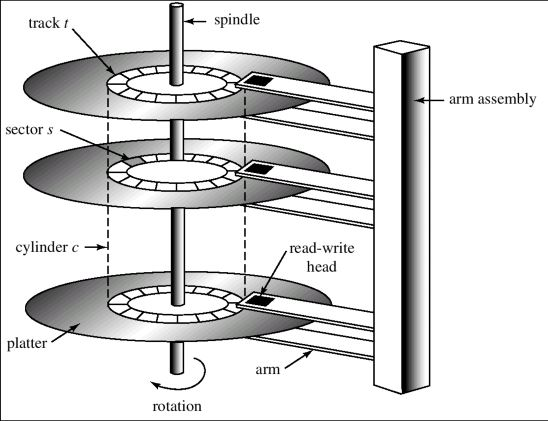
\includegraphics[width=7cm]{img/disk.JPG}
\end{wrapfigure}
Le operazioni di lettura e scrittura sono rese possibili da una testina sospesa sulla superficie magnetica. Per scrivere, viene fatta passare corrente attraverso la testina per magnetizzare la superficie. Per la lettura, il passaggio sopra un'area magnetizzata induce una corrente positiva o negativa nella testina.

La testina è attaccata a un \textit{braccio}. La superficie di un piatto è logicamente divisa in tracce circolari, a loro volta divise in settori. L'insieme di tracce che si trovano alla stessa posizione del braccio formano un cilindro. Potrebbero esserci migliaia di cilindri concentrici in un disco magnetico e ogni traccia potrebbe contenere centinaia di settori. 

Quando un disco è in uso, un motore lo fa girare ad alta velocità, la quale viene calcolata in rotazioni al minuto. Quando si parla di velocità, tuttavia, bisogna considerare anche altri (più importanti) parametri. La \textbf{velocità di trasferimento (transfer rate)} è la velocità con cui i dati sono trasferiti dal disco al computer e viceversa. Il \textbf{tempo di posizionamento}, o random access time, consiste di due parti: il tempo necessario a spostare fisicamente il braccio sul cilindro desiderato, chiamato \textbf{seek time}, e il tempo impiegato dal settore per ruotare fino ad arrivare sotto alla testina, detto \textbf{rotational latency}.\newline
Il tempo di accesso è dato quindi dalla seguente formula: \newline
$ T_{accesso} = T_{seek} + T_{latency} + T_{transfer} $

\paragraph{Esempio}
\begin{itemize}
\item velocità di traferimento = 40MB/s
\item Velocità di rotazione = 10000rpm = 166 rps
\item Rotazione media = 1/2 traccia
\item Dimensione blocco = 512 bytes
\item Seek time = 5ms
\end{itemize}
$ T_{accesso} = 5 ms + 0.5/166 + 0.5 KB/40 MB = 5 ms + 3 ms + 0.0000125 = 8.0000125 ms $ 
\newline

Il seek time è dominante, quindi, dato il grande numero di processi nel sistema che accedono al disco, è necessario minimizzarlo tramite algoritmi di scheduling atti a minimizzare il tempo di accesso totale e massimizzare la banda (cioè il numero di byte trasferiti per unità di tempo).

Poiché la testina è sospesa a pochi micron dalla superficie del disco, c'è il pericolo che avvenga un contatto tra le due parti. Anche se i piatti sono coperti da un materiale protettivo, la testina potrebbe comunque danneggiare la superficie. In questo caso si parla di \textbf{head crash}. Non c'è modo di riparare a tal tipo di incidente, se non cambiando il disco.

I moderni dischi magnetici sono generalmente raggruppati dal punto di vista logico in cluster, settore dopo settore, tanto che può essere considerato quasi un array unidimensionale di indirizzamento. Per accedere a un settore bisogna specificare superficie, traccia e il settore stesso.

\paragraph{Dispositivi a stato solido}
Stanno prendendo sempre più piede. Utilizzano dei chip (DRAM o memorie flash NAND) per memorizzare i dati in modo non volatile. Gli SSD hanno le stesse caratteristiche degli hard disk tradizionali ma possono essere più affidabili perché non hanno marti in movimento e più veloci perché non sono afflitti dal tempo di ricerca o dalla latenza data dal movimento di testine e dischi. Come se non bastasse, consumano molta meno energia. Usano la stessa interfaccia dei dischi fissi e quindi possono rimpiazzarli facilmente. Per ora la capacità arriva fino ai 2TB, ma la grandezza massima acquistabile a un prezzo ragionevole è 256GB.


\subsection{Scheduling degli accessi a disco}
Il Sistema Operativo deve utilizzare l'hardware a disposizione nella maniera più efficiente possibile. Per i dischi magnetici, questo significa minimizzare il tempo di accesso e massimizzare la banda. Come già visto, il tempo di accesso è influenzato per la maggior parte dal tempo richiesto al braccio per muovere la testina sul cilindro giusto (seek time) e dal tempo necessario a far girare il disco per spostare il settore desiderato sotto alla testina (rotational latency). La banda, come già detto, è il numero totale di bytes trasferiti, divisi per il tempo totale dalla prima richiesta del servizio al completamento dell'ultimo trasferimento. 

Quando un processo richiede un'operazione di I/O da o verso il disco, effettua una chiamata di sistema. La richiesta specifica diverse informazioni:
\begin{itemize}
\item Tipo di accesso (lettura o scrittura)
\item L'indirizzo sul disco
\item L'indirizzo in memoria
\item Il numero di settori da trasferire
\end{itemize}

Per i seguenti algoritmi si considerano i seguenti accessi (espressi come numero di cilindro/traccia): \newline
\centerline{98, 183, 37, 122, 14, 124, 65, 67}
\newline
Con l'intervallo [0, 199] di valori ammissibili e la testina inizialmente posizionata sulla traccia 53.

\subsubsection{First Come, First Served (FCFS)}
L'algoritmo più semplice soddisfa le richieste nell'ordine in cui arrivano. L'algoritmo è \textit{fair}, ma generalmente non è il più veloce.

\subsubsection{Shortest Seek Time First (SSTF)}
Sembra ragionevole soddisfare per prime le richieste vicine alla testina. Questo algoritmo seleziona quindi le richieste soddisfacibili con il minore seek time, considerando la posizione corrente della testina. In pratica, segue lo stesso principio dello Shortest Job First (SJF) e come esso soffre del problema della possibile starvation. Anche se è un sostanziale miglioramento rispetto a FCFS, l'algoritmo SSTF non è ancora ottimale.

\subsubsection{Scheduling SCAN e LOOK}
In questo algoritmo, la testina parte da un'estremità del disco e si sposta verso l'altra estremità, servendo tutte le richieste correnti. Arrivata all'altra estremità, riparte nella direzione opposta, servendo le nuove richieste. Per questa sua natura è spesso chiamato algoritmo dell'ascensore.

\paragraph{C-SCAN} Come variante dell'algoritmo SCAN, nello SCAN Circolare (C-SCAN) la testina, una volta arrivata alla seconda estremità, si sposta direttamente alla prima e ricomincia, trattando quindi il disco come una lista circolare.

\paragraph{LOOK e C-LOOK} Gli algoritmi LOOK e C-LOOK sono varianti, rispettivamente, di SCAN e C-SCAN, in cui la testina non arriva all'estremità del disco, ma cambia direzione (LOOK) o riparte dalla prima traccia (C-LOOK) non appena non ci sono più richieste in quella direzione.
\newline

Alla pagina seguente si trovano gli schemi di funzionamento degli algoritmi appena esposti.
\begin{figure}
\centering
  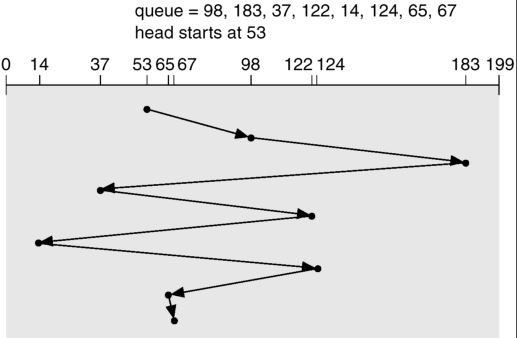
\includegraphics[width=5cm]{img/fcfs.JPG}
\caption{Scheduling FCFS}
  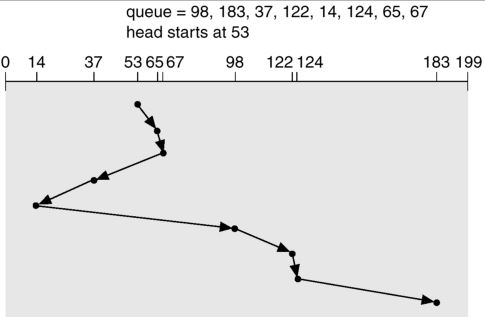
\includegraphics[width=5cm]{img/sstf.JPG}
\caption{Scheduling SSTF}
  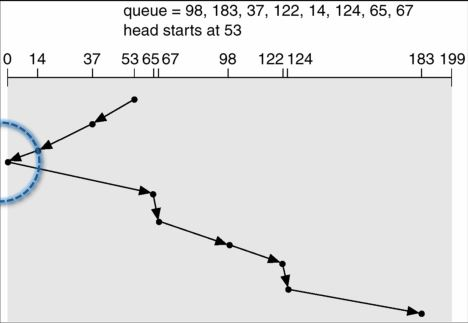
\includegraphics[width=5cm]{img/scan.JPG}
\caption{Scheduling SCAN}
  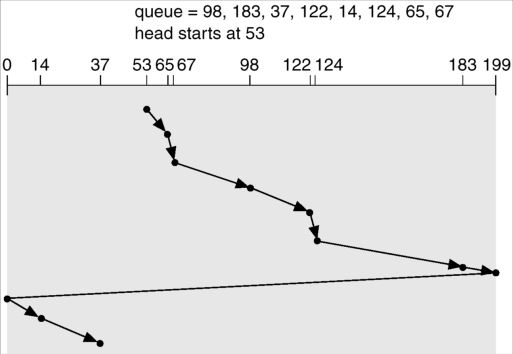
\includegraphics[width=5cm]{img/cscan.JPG}
\caption{Scheduling C-SCAN}
  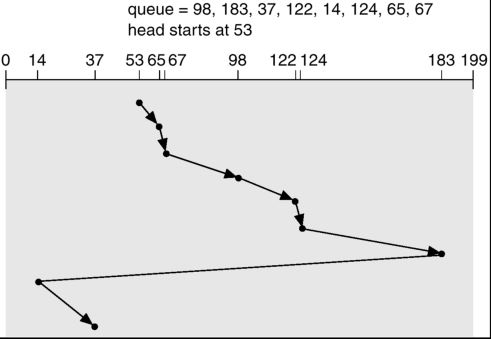
\includegraphics[width=5cm]{img/clook.JPG}
\caption{Scheduling C-LOOK}
\end{figure}
\newline

Esistono altre varianti dello SCAN in cui, per evitare che la testina rimanga sempre nella stessa zone, la coda delle richieste viene partizionata in più code di dimensione massima N. Quando una coda viene processata per il servizio (scan in una direzione), gli accessi in arrivo riempiono altre code. Le code ``sature'' vengono servite nello san successivo, considerando che con N grande degenera in SCAN e con N=1 si ha un esempio di FCFS. Questo algoritmo prende il nome di \textbf{N-step SCAN}. Se si utilizzano solo due code, si parla invece di \textbf{FSCAN}.

\paragraph{LIFO} In alcuni casi, può essere utile schedulare gli accessi in base all'ordine inverso di arrivo, soprattutto nel caso di accessi con elevata località. Ovviamente, tale approccio aumenta di molto la possibilità di starvation.

\subsubsection{Analisi degli algoritmi}
Nessuno degli algoritmi presentati è ottimo, ogni caso ha il proprio algoritmo più adatto. SSTF è di uso comune e risulta appetibile perché migliora le prestazioni di FCFS. SCAN e C-SCAN forniscono performance migliori per sistemi con un alto numero di accessi al disco perché hanno una bassissima probabilità di generare casi di starvation. 

Le richieste per il servizio possono inoltre essere influenzate dall'organizzazione delle informazioni su disco. Ad esempio, un programma che legge un file allocato contiguamente, genererà numerose richieste vicine sul disco. 

L'algoritmo di scheduling del disco dovrebbe essere scritto come un modulo indipendente dal Sistema Operativo, così da poter essere rimpiazzato di volta in volta con la scelta migliore.


\subsection{Gestione del disco}

\subsubsection{Formattazione dei dischi}
Prima di poter contenere dei dati, un disco deve essere diviso in settori che possano essere scritti e letti dal disk controller. Questo processo è chiamato formattazione di basso livello o fisica. Questo tipo di formattazione riempie il disco con una struttura dati speciale per ogni settore, la quale consiste di un header, un'area dati (solitamente 512 bytes) e un trailer. L'header e il trailer contengono informazioni utilizzate dal controllore, quali il numero del settore ed un codice di correzione dell'errore (ECC). Quando il correttore scrive in settore di dati durante una normale operazione di I/O, l'ECC viene aggiornato con un valore calcolato a partire da tutti i bytes nell'area dati. Quando il settore viene letto, l'ECC è ricalcolato e comparato con il valore memorizzato. Se i due valori calcolati non coincidono, l'area dati del settore potrebbe essere corrotta. L'ECC è un un codice di correzione degli errori perché contiene abbastanza informazioni per permettere al controllore di individuarli e correggerli, se pochi bit di dati sono corrotti. Un errore recuperabile come quello descritto è detto \textbf{soft error}.

Prima di poter tenere files in un disco, il sistema operativo ha bisogno di registrare i propri dati nel disco stesso ed esegue questo in due steps. Il primo passo è partizionare il disco in uno o più gruppi di cilindri. Il secondo step è la formattazione logica, o la creazione di un file system. In questo step, il sistema operativo memorizza le strutture iniziali del file system sul disco. Queste strutture di dati possono includere mappe dello spazio vuoto e allocato e una directory iniziale vuota.

Per fa sì che un computer possa avviarsi, deve esserci un programma iniziale da eseguire. Questo programma, detto \textbf{bootstrap program}, tende and essere piuttosto semplice. Esso inizializza tutti gli aspetti del sistema, dai registri della CPU ai controller di device e i contenuti della memoria principale, quindi avvia il sistema operativo. 

Nella maggior parte dei computer, il bootstrap è ospitato nell ROM. Questa locazione è particolarmente conveniente, sia perché non ha bisogno di inizializzazione, sia perché ha una locazione fissa per cui il processore può eseguirla fin da subito, sia perché essendo di sola lettura non può essere infettata da virus.

\subsubsection{Gestione dei blocchi difettosi}
Poiché i dischi hanno parti in movimento con pochissimo margine di tolleranza, sono proni all'errore. A volte questo può essere fatale, obbligando quindi l'utente a sostituire il disco. Altre volte, solo dei settori diventano difettosi. La maggior parte dei dischi esce addirittura dalla fabbrica con dei blocchi difettosi. Ci sono vari modi di gestire questi particolari blocchi.

Su dischi semplici, i blocchi difettosi sono gestiti manualmente. Una strategia è quella di scansionare tutto il disco alla ricerca dei blocchi incriminati, durante la formattazione. Ogni bad block scoperto è marcato come inutilizzabile, così che il file system non possa allocarlo. Se i blocchi vengono corrotti durante una normale operazione, è necessario eseguire manualmente uno speciale programma per cercare i blocchi e marcarli.

Nella gestione detta on-line, il controllore mantiene una lista con tutti i blocchi corrotti. La lista è inizializzata durante la formattazione di basso livello e viene aggiornata durante la vita del disco. La formattazione di basso livello riserva inoltre dei blocchi d'avanzo, invisibili al file system, che il controllore può utilizzare in seguito per rimpiazzare i blocchi corrotti. Questo schema è noto col nome di \textbf{sector sparing} o \textbf{forwarding}.

\subsubsection{Gestione dello spazio di swap}
 Lo swapping è stato inizialmente presentato quando si doveva spostare interi processi tra il disco e la memoria principale. Lo swapping in quel contesto è necessario quando la quantità di memoria fisica raggiunge dei livelli critici, quindi i processi sono spostati dalla memoria allo spazio di swap per liberarla. In realtà, tuttavia, ben pochi sistemi adoperano questa soluzione. Piuttosto, i sistemi ora combinano lo swap con tecniche di memoria virtuale e swappano solo delle pagine, non interi processi.
 
 Uno spazio di swap può risiedere in due posti differenti: può essere ricavato dall'interno del normale file system, o potrebbe trovarsi in una diversa partizione del disco. Se lo spazio di swap è semplicemente un grande file all'interno del file system, possono essere utilizzate delle normali routines per crearlo, nominarlo e allocarlo. Questo approccio, anche se facile da implementare, è inefficiente, poiché prevede di navigare nella struttura delle directory, comportando numerosi accessi al disco.
 
 Alternativamente, si può creare uno spazio di swap in una partizione apposita. Nessun file system o directory verrà posizionata in questa area e un manager separato viene utilizzato per allocare e deallocare i blocchi dalla partizione.

Lo spazio di swap viene poi allocato quando un processo viene creato o quando una pagina viene forzata fuori dalla memoria fisica. Nel primo caso, viene assegnato dello spazio per le pagine di istruzioni e dati e il kernel utilizza due mappe di swap per tracciare l'uso dello spazio di swap.








\newpage
\section{Livelli RAID}

\begin{figure}[htb]
\centering
  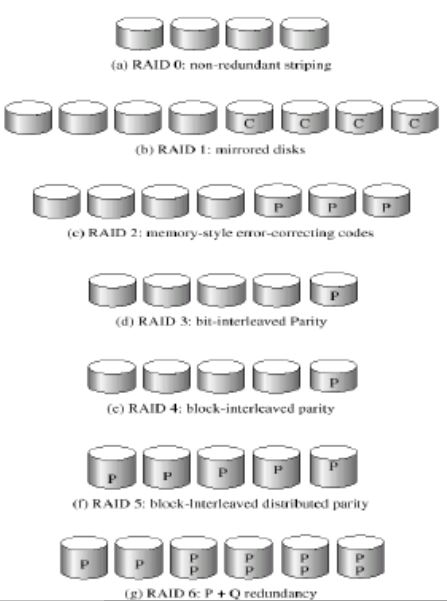
\includegraphics[width=8cm]{img/raid.JPG}
\end{figure}

Dato il progressivo decremento del costo dei dischi, è ora possibile aggiungerne diversi a un qualsiasi computer. Avere un gran numero di dischi in un sistema presenta numerose opportunità per migliorare la velocità di lettura/scrittura, se i dischi lavorano in parallelo. Inoltre, permettono una maggiore affidabilità, poiché è possibile registrare informazioni ridondanti in più dischi. 

Una varietà di tecniche di organizzazione dei dischi, comunemente chiamata \textbf{redundant arrays of independent disks (RAID)}, è utilizzata per parlare di problemi di prestazioni ed affidabilità.

La soluzione al problema dell'affidabilità è la ridondanza. La soluzione più semplice (e più costosa), per ottenerla è la duplicazione di ogni disco (\textbf{mirroring}). Con il mirroring, ogni disco logico si compone in realtà di due dischi fisici e ogni scrittura è effettuata su entrambi. 

L'accesso parallelo a più dischi migliora le prestazioni. Con il mirroring dei dischi, la velocità di lettura può essere duplicata, dato che le richieste possono essere mandate a entrambi i dischi. 

Con l'utilizzo di dischi multipli, inoltre, è possibile migliorare la capacità di trasferimento distribuendo i dati in sezioni su più dischi (\textbf{data striping}). Il sezionamento può essere fatto a livello di bit (distribuzione di bit disco per disco) o a livello di blocco (distribuzione di blocchi disco per disco). 

Il bilanciamento del carico aumenta la produttività per accessi multipli a piccole porzioni di dati e viene ridotto il tempo di risposta relativo agli accessi a grandi quantità di dati.

In somma, il mirroring fornisce alta affidabilità, ma è costoso (in tutti i sensi). Il data striping assicura invece unìalta capacità di trasferimento dei dati, ma non migliora l'affidabilità. Sono state proposte numerose tecniche per fornisce la ridondanza a un basso costo utilizzando il data striping in combinazione con dei bit di parità. Queste tecniche sono classificate nei livelli di RAID.

\begin{itemize}
\item \textbf{RAID Livello 0} -- Il sezionamento viene fatto a livello del blocco e non vi è ridondanza. Risulta economico e con alte prestazioni, date dal parallelismo, ma non ha ridondanza e l'affidabilità cala all'aumentare del numero di dischi impiegati.
\item \textbf{RAID Livello 1} -- In questo caso c'è mirroring, ma manca il sezionamento. Questa soluzione è costosa, garantisce una maggiore affidabilità e maggiori prestazioni in lettura.
\item \textbf{RAID Livello 2} -- Ad ogni byte è associato un bit che indica se gli 1 presenti nel byte sono in numero pari (parità 0) o dispari (parità 1), quindi identifica tutti gli errori sul singolo bit. Si possono correggere più bit, utilizzando bit di parità supplementari. L'idea dell'ECC può essere utilizzata direttamente in array di dischi tramite lo striping dei bytes. Ad esempio, il primo bit di ogni byte può trovarsi nel disco 1, il secondo nel disco 2 e così via fino all'ottavo. I bit di correzione dell'errore sono memorizzati in un altro disco. Un RAID di livello 2 è quindi un RAID 0 con maggiore affidabilità.
\item \textbf{RAID Livello 3} -- In questo livello il sezionamento è fatto a livello di byte con un disco dedicato al bit di parità. I controllori dei dischi sono in grado di rilevare se un settore è stato letto correttamente: se un settore è danneggiato, per ogni bit del settore è possibile determinare se deve valere 0 o 1 calcolando la parità dei bit corrispondenti dai settori degli altri dischi. Se la parità dei rimanenti bit è uguale a quella memorizzata, allora il bit mancante è 0, altrimenti è 1. Questo livello ha la stessa efficienza di RAID 2, ma usa un solo disco per i bit di parità, mentre la velocità di trasferimento è pari a n volte quella di RAID 1, grazie al data striping. Rispetto al RAID 1, tuttavia, può effettuare meno operazioni di I/O al secondo perché ogni disco è coninvolto in tutte le richieste ed il tempo per le scritture è più lungo perché è necessario calcolare il bit di parità (anche se di questo può occuparsi il controllore RAID, al posto della CPU).
\item \textbf{RAID Livello 4} -- Utilizza il sezionamento a livello di blocco, con un disco dedicato alla parità. Se un disco viene corrotto, il blocco di parit può essere utilizzato per recuperarne i blocchi. Come nel livello 3, il calcolo della parità influisce sulla velocità di lettura e anzi, il disco riservato per i bit di parità può fare da collo di bottiglia.
\item \textbf{RAID Livello 5} -- Il sezionamento viene fatto a livello di blocco, con i bit di parità distribuiti tra tutti i dischi. Un blocco di parità non può contenere informazioni di parità per blocchi che risiedono nello stesso disco, altrimenti un guasto al disco farebbe perdere i dati. Questa soluione va quindi ad eliminare il problema del collo di bottiglia del RAID 4, ma persiste il problema della scrittura lenta.
\item \textbf{RAID Livello 6} -- Simile al RAID 5, ma con maggiori informazioni di ridondanza per gestire guasti contemporanei su più dischi. Al posto della parità, utilizza altri codici per la correzione dell'errore (Reed-Solomon). Garantisce un'altissima ridondanza, ma va ad aumentare il costo. Inoltre, la gestione dei codici per la correzione degli errori va a rallentare ancora di più la scrittura.
\item \textbf{RAID Livello 0+1 e 1+0} -- Il RAID 0+1 combina RAID 0 e RAID 1 per fornire affidabilità e alte prestazioni. Una tale configurazione, tuttavia, richiede il raddoppio del numero di dishci necessari per memorizzare i dati e non supporta la rottura simultanea di due dischi se non appartengono allo stesso stripe.

Il RAID 1+0 combina RAID 1 e RAID 0, risultando più robusto di RAID 0+1, infatti ogni disco di ogni stripe può guastarsi senza far perdere dati al sistema.
\end{itemize}







\newpage
\section{File System}
Il file system fornisce il meccanismo per la memorizzazione e l'accesso di dati e programmi. Consiste di due parti distinte: una collezione di file e una struttra di cartelle (directory). 

\subsection{L'interfaccia del file system}

\subsubsection{Il concetto di file}
Affinché il computer possa essere convenientemente utilizzato, il sistema operativo fornisce una vista logica uniforme delle informazioni memorizzate. Il sistema operativo astrae dalle caratteristiche fisiche dei supporti di memorizzazione per una unità logica di memorizzazione, il \textbf{file}.

Un file è un insieme di informazioni correlate, identificate da un nome, memorizzate in un dispositivo di memorizzazione secondario. Comunemente, i files rappresentano sia programmi, sia dati. I file di dati potrebbero essere testuali, numerici, multimediali, binari, eccetera. In generale, un file è una sequenza di bits, bytes, linee o campi, il cui significato è definito dal creatore del file e dall'utilizzatore. 

Un file ha una certa struttura definita in base al suo tipo.

\paragraph{Attributi dei files}
Quando a un file viene assegnato un nome, esso diventa indipendente dal processo, dall'utente e addirittura dal sistema che lo ha creato. 

Gli attributi di un file variano in base al sistema operativo, ma è corretto pensare che questi siano validi per ognuno:
\begin{itemize}
\item \textbf{Nome}: è l'unica informazione in formato ``leggibile'' dall'utente
\item \textbf{Tipo}
\item \textbf{Posizione}: un puntatore allo spazio fisico sul dispositivo
\item \textbf{Dimensione}
\item \textbf{Protezione}: informazioni per il controllo degli accessi (permessi di lettura/scrittura)
\item \textbf{Tempo, data e identeificazione dell'utente}
\end{itemize}

\paragraph{Operazioni su file}
Un file è un tipo di dato astratto. Il sistema operativo può fornire delle chiamate di sistema per creare, scrivere, leggere, riposizionare, cancellare e troncare files.
\begin{itemize}
\item \textbf{Creazione}. Si ricerca dello spazio su disco, quindi viene creato un nuovo elemento nella directory
\item \textbf{Scrittura}. La sysem call apposita specifica sia il nome del file che le informazioni che devono esservi scritte. Il sistema deve mantenere un puntatore di scrittura alla posizione nel file in cui deve avvenire la struttura successiva.
\item \textbf{Lettura}. La chiamata di sistema specifica il nome del file e dove mettere i dati letti in memoria. Il sistema deve mantenere un puntatore alla locazione della prossima lettura, come per la scrittura. Poiché in genere un file non viene letto e scritto contemporaneamente, la posizione dell'operazione corrente può essere mantenuta con un solo puntatore per processo (anziché uno per la lettura e uno per la scrittura).
\item \textbf{Riposizionamento all'interno di un file}. Operazione nota anche come \textit{seek}, consiste nell'aggiornare il puntatore alla posizione corrente.
\item \textbf{Cancellazione}. Libera lo spazio associato al file e l'elemento corrispondente nella directory.
\item \textbf{Troncamento}. Mantiene inalterati gli attributi, tuttavia cancella il contenuto del file.
\end{itemize}

Altre comuni operazioni sono la concatenazione a fine file e la rinominazione di un file. Si possono inoltre creare copie di un file, o addirittura copiarlo verso un altro dispositivo (stampanti, display, ecc.).

La maggior parte delle operazioni citate finora includono la ricerca dell'elemento con il nome specificato nella struttura delle directory. Per evitare questa costante ricerca, molti sistemi operativi richiedono che sia invocata la chiamata di sistema \texttt{open()} prima di un qualsiasi utilizzo di un file. Il sistema operativo mantie euna tabella, chiamata \textbf{open-file table}, che contiene tutte le informazioni riguardanti i file aperti. Quando viene richiesta un'operazione su un file, questo è specificato tramite un indice nella tabella e non c'è bisogno di ricercarlo ogni volta. Quando un file non è più utilizzato, viene chiuso dal processo e il sistema operativo può rimuovere l'elemento a esso associato dalla tabella. 

Tipicamente, il sistema operativo utilizza due livelli di tabelle: una per processo e una per l'intero sistema. La tabella per-processo tiene traccia dei files aperti da quello specifico processo (puntatori alla locazione di lettura/scrittura). 

Ogni elemento nella tabella del processo punta a una tabella di sistema, che contiene le informazioni indipendenti del file, cioè la posizione sul disco, la dimensione, informazioni di data e ora. Tipicamente ogni elemento è associato anche a un valore, detto \textbf{open count} che tiene traccia dei processi che hanno aperto il file. Ogni chiamata \texttt{close()} decrementa l'open count e quando esso arriva al valore 0, l'elemento è rimosso dalla tabella di sistema dei file aperti.

Quando un file viene chiuso, esso viene copiato dalla memoria al disco.

\paragraph{Struttura di un file}
I tipi di file possono essere adoperati per indicare la struttura interna del file. Le strutture possibili sono le seguenti:
\begin{enumerate}
\item Nessuna, cioè un file è una sequenza parole, bytes, ecc... Unix usa questa struttura.
\item Struttura a ``record'' semplice, dove record è un sinonimo per riga e può essere di lunghezza fissa o variabile
\item Strutture complesse. Ad esempio, documenti formattati e formati ricaricabili.
\end{enumerate}
Spesso è possibile emulare le strutture 2 e 3 utilizzando la 1, servendosi di specifici caratteri di controllo.

\subsubsection{Metodi di accesso}
Si può accedere all'informazione contenuta in un file in diversi modi.
\paragraph{Accesso sequenziale}
L'informazione nel file è processata in ordine, un record dopo l'altro. Questa modalità, che è la più diffusa, è utilizzata anche dalla maggior parte degli editor e dei compilatori. Le operazioni permesse sono: \texttt{read\_next()}, \texttt{write\_next()} e \texttt{reset()}, la quale rimette il puntatore all'inizio del file.

Non è permesso il rewrite poiché si rischierebbe di sovrascrivere anche record successivi che magari vanno lasciati intoccati.

\paragraph{Accesso diretto}
In questa modalità, il file è visto come una sequenza numerata di blocchi (records), i quali possono essere letti e scritti senza un particolare ordine. Le operazioni permesse si riferiscono sempre all'n-esimo blocco e sono, ad esempio: \texttt{read(n), write(n), position\_to(n), read\_next(), write\_next(), rewrite(n)}.

\subsection{Struttura delle directory}
Un dispositivo di memorizzazione può essere interamente utilizzato per un file system. Può anche, tuttavia, essere suddiviso per un miglior controllo. Ad esempio, un disco potrebbe essere partizionato in quarti e ogni quarto potrebbe contenere un file system differente.

Il partizionamento è utile per limitare la dimensione dei file system individuali, per mettere più file system in uno stesso dispositivo, o per lasciare parte del dispositivo libera per altri usi. Un'entità contenente un file system è generalmente chiamata \textbf{volume}. 

Ogni volume che contiene un file system, deve anche contenere informazioni sui file nel sistema. Queste informazioni sono mantenute in elementi della \textbf{tabella dei contenuti del volume} (device directory o volume table of contents). La device directory registra informazioni su tutti i file del volume.

Una directory può essere vista come una tabella di simboli che traduce i nomi dei file in elementi della relativa cartella. La cartella stessa può essere organizzata in molti modi. L'organizzazione deve permettere di inserire, cancellare, ricercare, rinominare ed elencare gli elementi. Un'altra operazione possibile è l'attraversare il file system, cioè avere la possibilità di accedere a qualsiasi file in una qualsiasi directory da un qualsiasi altro punto del file system.  

\paragraph{Organizzazione logica di una directory}
Gli obiettivi da conseguire quando si organizza una directory sono: efficienza (rapido accesso ai file), nomenclatura (che sia conveniente per gli utenti), raggruppamento (classificazione logica dei file per criterio).
\newline

\textbf{Directory a un livello}\newline
Questa è sicuramente la struttura più semplice. Tutti i file sono contenuti nella stessa directory. Ovviamente ci sono grandi problemi di nomenclatura, poiché ogni file dovrà avere un proprio nome unico, e di raggruppamento (inesistente).
\newline

\textbf{Directory a due livelli}\newline
In questa struttura, ogni utente ha la propria user file directory (UFD). Ogni UFD è poi una directory a un livello, con tutte le limitazioni che ne conseguono. Rimane un problema: dove vengono messi i programmi di sistema condivisi da più utenti?
\newline

\textbf{Directory ad albero}\newline
Una naturale generalizzazione della struttura a due livelli è quella ad albero. Questa permette di effettuare ricerche in maniera efficiente e dà la possibilità di effettuare raggruppamenti logici. Introduce, inoltre, il concetto di directory corrente (working path) e quindi quello di percorso assoluto e relativo. 
\newline

\textbf{Directory a grafo aciclico}
Una normale struttura ad albero non permette la condivisione di file e directory. Per questo motivo l'albero viene esteso a un grafo aciclico. L'implementazione della condivisione è fatta in diversi modi a seconda del sistema operativo utilizzato:
\begin{itemize}
\item Link simbolico (Windows): contiene il pathname del file/directory reale. Se l'originale viene cancellato, il link rimane pendente.
\item Hard link (Unix): un contatore mantiene il numero di riferimenti e il file può essere cancellato solo se il valore è 0 (quindi non lascia link pendenti).
\end{itemize} 

\textbf{Directory a grafo generico}
 Un'ulteriore generalizzazione, in cui è però necessario garantire che non esistano cicli, al fine di evitare loop infiniti nell'attraversamento del grafo. A tale scopo, è permesso collegare solo file e non directory e si può utilizzare un algoritmo di controllo ogni volta che si crea un nuovo collegamento (molto costoso).
 
\subsubsection{Mount di file system}
Così come un file deve essere aperto prima di venir utilizzato, allo stesso modo un file system deve essere \textit{montato} prima che possa essere disponibile ai processi del sistema. Nello specifico, la struttura delle directories deve essere costruita a partire dai vari volumi, che devono essere montati per fare in modo che siano disponibili nel name-space del file system.

La procedura di mounting è diretta. Il sistema operativo riceve il nome di un device e il \textbf{mount point} -- cioè il punto in cui viene attaccato il file system. Tipicamente, il mount point è una cartella vuota. 

Il Sistema Operativo verifica quindi che il device contenga un file system valido, per poi annotare nella propria struttura delle directories che quel file system è stato attaccato a uno specifico mount point.

\subsubsection{Condivisione di file}
La condivisione di files è molto importante in sistemi multiutente.

Quando un sistema operativo ospita più utenti, la condivisione dei files porta degli ostacoli da superare: il \textit{file naming} e, soprattutto, la protezione.

Per implementare la condivisione e la protezione, il sistema deve mantenere più attributi di file e cartelle rispetto a sistemi monoutente. Anche se sono stati adottati molti approcci diversi per rispondere a questi requisiti, la maggior parte dei sistemi operativi è arrivata ad utilizzare il concetto di \textbf{proprietario (owner)} e \textbf{gruppo (group)}. Il proprietario è l'utente che può cambiare gli attributi, garantire l'accesso al file o alla directory e in generale ha un controllo primario sul file. Il gruppo definisce un insieme di utenti che possono accedere al file.

\subsubsection{Protezione}
Ovviamente, si vuole poter tenere al sicuro le informazioni presenti in un computer. In particolare, si vuole poter controllare cosa è possibile fare su un file e chi può farlo. 

Il desiderio di protezione è strettamente legato all'abilità di accedere ai files. I sistemi che non permettono di accedere ai files ad altri utenti ad eccezione del creatore, non hanno bisogno di protezione, quindi si può fornire una protezione completa bloccando ogni accesso. Al contrario, si può garantire l'accesso libero, rinunciando di fatto a ogni tipo di protezione (che non derivi da eventuali copie di backup dei files). Entrambi gli approcci sono ovviamente troppo estremi per un uso generale, c'è quindi bisogno di poter controllare gli accessi in maniera selettiva.

I meccanismi di protezione forniscono degli accessi controllati limitando il tipo di accessi possibili. In particolare, è possibile controllare le seguenti operazioni:
\begin{itemize}
\item Lettura
\item Scrittura
\item Esecuzione
\item Append (aggiunta in coda)
\item Cancellazione
\end{itemize}

L'approccio più comune per la protezione è rendere l'accesso possibile in base all'identità dell'utente. Per implemetare tale soluzione, a ogni file viene associata una lista d'accesso (ACL -- Access Control List), in cui sono specificati gli utenti e i loro relativi permessi di accesso. Quando un utente richiede di accedere a un particolare file, il sistema operativo controlla la ACL associata ed eventualmente permette (o nega) l'accesso. 

Il problema principale delle ACLs è la loro lunghezza. Per condensare la lista, si possono dividere gli utenti nella seguente classificazione:
\begin{itemize}
\item Proprietario
\item Gruppo
\item Universo
\end{itemize}

Si può quindi associare ogni categoria alle operazioni ad essa possibile. Ad esempio, nei sistemi Unix le operazioni possibili sono: r (read), w (write), x (execute); eseguendo a terminale il comando: \texttt{chmod 754 nome\_file rwx r-x r-{}-}, il proprietario ha il permesso di fare tutto, il gruppo non può scrivere e l'universo può solo leggere.

\subsection{Implementazione del file system}

\begin{figure}[htb]
\centering
  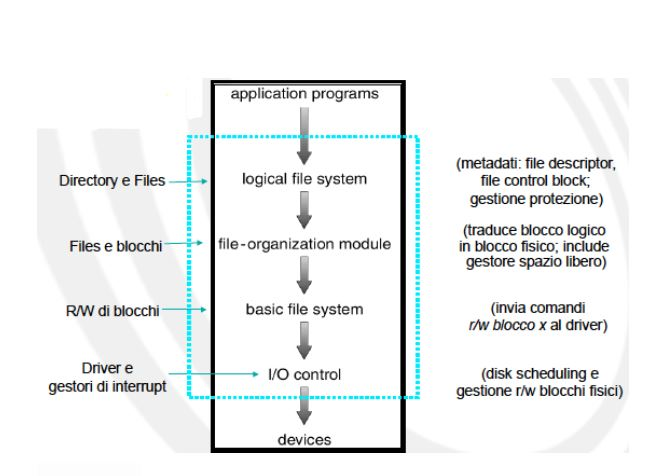
\includegraphics[width=8cm]{img/filesys.JPG}
\end{figure}

Per migliorare l'efficienza dell'I/O, le transazioni tra la memoria e il disco sono fatte in unità chiamate blocchi. Ogni blocco ha uno o più settori (la cui grandezza, comunemente, è di 512 bytes).

Generalmente, il file system stesso si compone di tanti livelli differenti. Ogni livello nel design utilizza funzionalità dei livelli sottostanti per crearne di nuove, utilizzate dai livelli superiori. 

Il livello del controllo dell'I/O contiene i drivers di device e i gestori degli interrupt per trasferire le informazioni tra la memoria e il disco. 

Il file system di base ha solo bisogno di dirigere dei comandi generici verso il device driver appropriato per leggere e scrivere il blocco fisico nel disco. Questo livello gestisce anche i buffer della memoria e le cache che contengono i vari file system, cartelle e blocchi di dati.

Il file-organization module conosce i files e i loro blocchi logici e fisici. Può tradurre l'indirizzo del blocco logico nell'indirizzo fisico del blocco, così che il basic file system possa effettuare il trasferimento. Include inoltre il gestore dello spazio libero.

Il logical file system gestisce i metadati, cioè file descriptors, file control block. Gestisce anche la struttura delle directories.

Una struttura a livelli come quella appena descritta permette di minimizzare la duplicazione di codice.
\newline

Per gestire un file system si utilizzano diverse strutture dati, sia su disco che in memoria. Le loro caratteristiche sono fortemente dipendenti dal sistema operativo e dal file system stesso, tutta via ne esistono alcune comuni a tutte le tipologie. 

Sul disco, il file system potrebbe contenere informazioni circa il boot del sistema operativo, il numero totale di blocchi, il numero e la posizione dei blocchi liberi, la struttura delle directories e i file individuali. In breve:
\begin{itemize}
\item Blocco di boot: contiene le informazioni necessarie per l'avviamento del S.O.
\item Blocco di controllo delle partizioni: contiene i dettagli del volume, quali il numero e la dimensione dei blocchi, la lista dei blocchi liberi, la lista dei descrittori liberi, eccetera.
\item Struttura delle directories (per ogni file system): descrive l'organizzazione dei files.
\item Descrittori di file: contengono dettagli sui file e puntatori ai blocchi di dati.
\end{itemize}

Le informazioni in memoria sono utilizzate sia per la gestione del file system che per il miglioramento delle prestazioni tramite cache. I dati sono caricati a tempo di mount, aggiornati durante le operazioni del file system e scartati al dismount.
\begin{itemize}
\item Tabella delle partizioni: contiene informazioni sulle partizioni montate
\item Struttura delle directories: una copia in memoria delle directory cui si è acceduto recentemente
\item Tabella globale dei file aperti
\item Tabella dei file aperti per ogni processo
\end{itemize}

\subsubsection{Allocazione dello spazio su disco}
 Esistono tre metodi principali per allocare lo spazio libero sul disco: allocazione continua, linkata e indicizzata. Gli obiettivi sono, ovviamente, la massimizzazione nell'utilizzo dello spazio e la minimizzazione dei tempi di accesso.
 
 \paragraph{Allocazione contigua}
Ogni file occupa un insieme di blocchi contigui su disco. Il numero di seek per accedere a un file sul disco è minimo. Se un file è lungo n blocchi e la posizione di partenza è b, allora occuperà b, b+1, b+2, ..., b+n-1. L'entry nella directory per ogni file indica solo l'indirizzo del blocco di partenza e la lunghezza totale dell'area allocata per il file.

L'accesso a un file risulta semplice: l'accesso al blocco b+1 è fattibile con una read\_next(), quindi non richiede uno spostamento della testina (a meno che non sia l'ultimo blocco di un cilindro). Ovviamente è supportato l'accesso sequenziale, così come quello casuale.

Come gli algoritmi di allocazione dinamica della memoria, l'allocazione contigua presenta degli sprechi, sia che si usi un best-fit, un first-fit o un worst-fit. Per risolvere il problema è necessario effettuare periodicamente una compattazione dello spazio libero.

Un altro problema è l'allocazione preventiva: quanto spazio allocare a un file che potrebbe crescere di dimensione in seguito? Esistono due possibilità. La prima prevedere che, nel caso il file dovesse crescere e non avesse spazio per farlo, il programma ritorni un errore e venga terminato. Il file verrà quindi spostato in un buco più grande. La soluzione è trasparente all'utente, ma rallenta il sistema.

Altri file system utilizzano uno schema modificato dell'allocazione contigua, basato sul concetto di extent (= serie di blocchi contigui su disco). Inizialmente, viene allocato un extent. Se quella quantità di spazio non è sufficiente, viene aggiunto un altro extent. A ogni blocco sono poi associati una posizione, un numero e un puntatore all'extent successivo, che non per forza sarà contiguo col precedente.

\paragraph{Allocazione a lista (o linkata)}
Questa modalità risolve tutti i problemi dell'allocazione contigua: ogni file è una lista di blocchi, i quali possono essere sparsi ovunque nel disco. La directory contiene i puntatori al primo e all'ultimo blocco e ogni blocco contiene un puntatore al successivo. 

La creazione di un nuovo file è semplice, in quanto basta cercare un blocco libero e creare una nuova entry nella directory. Allo stesso modo, è semplice l'estensione del file, in quanto basta cercare un altro blocco libero.

Non ci sono sprechi, ad eccezione dello spazio per il puntatore: è possibile utilizzare un qualsiasi blocco, andando ad eliminare la frammentazione esterna.

Purtroppo, questa modalità non supporta l'accesso casuale: bisogna ``saltare'' di puntatore in puntatore, a partire dal primo blocco e, poiché i blocchi sono sparsi, richiede molti riposizionamenti (seek). Questo tipo di allocazione soffre anche di scarsa affidabilità: basta perdere un puntatore o prelevarne uno sbagliato per compromettere un file. Una soluzione parziale è quella di utilizzare una lista doppiamente concatenata, mentre un'altra prevede la memorizzazione del nome del file e del numero di blocco in ogni singolo blocco del file, producendo un overhead assurdo.

Un'importante variazione dell'allocazione a lista è l'utilizzo di una \textbf{tabella di allocazione dei file (file allocation table -- FAT)}. Una sezione di disco all'inizio di ogni partizione è riservata per contenere la citata tabella. Questa ha una entry per ogni blocco ed è indicizzata in base al numero di questi. La directory entry contiene il numero di blocco del primo del file. L'entry della tabella indicizzata per quel blocc contiene il numero del blocco successivo, e la catena va avanti così. Per l'allocazione di un nuovo blocco basta scorrere la tabella e trovarne uno libero. 

L'allocazione con FAT ha come effetto collaterale l'elevato numero di seek, a meno che la FAT non sia messa in cache: per ogni blocco, la testina dovrebbe spostarsi da esso all'inizio della partizione, dove si trova la FAT. Il tempo di accesso casuale è invece molto migliorato.

\paragraph{Allocazione indicizzata}
\begin{wrapfigure}{r}{5,5cm}
\centering
  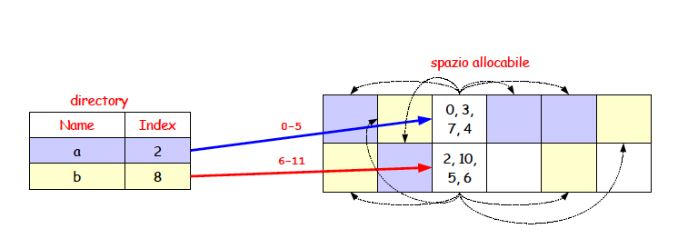
\includegraphics[width=7cm]{img/allocind.JPG}
\end{wrapfigure}
In questo tipo di allocazione, ogni file ha un blocco indice (index block) contenente la tabella degli indirizzi (index table) dei blocchi fisici. Ogni file ha il proprio blocco indice, contenuto come entry nella directory.

Supporta l'accesso dinamico e casuale, senza soffrire di frammentazione esterna poiché ogni blocco libero del disco può soddisfare una richiesta per dello spazio aggiuntivo. 

La dimensione del blocco indice limita la dimensione del file: se il blocco può contenere 512 parole, la dimensione massima del file sarà 512*512 parole = 256K parole. Esistono delle soluzioni per permettere di memorizzare file più grandi.
\begin{itemize}
\item \textbf{Indici multilivello}: un blocco indice di primo livello rimanda ad altri blocchi indice di secondo livello, i quali rimandano quindi ai blocchi del file.
\item \textbf{Schema concatenato}: Consiste nel fare una lista linkata di blocchi indice, cioè l'ultimo degli indici di un blocco punta a un altro blocco indice.
\item \textbf{Schema combinato}: ne sono un esempio gli i-node Unix. Per indirizzare i blocchi di dati del file, ogni i-node contiene 10 puntatori diretti a blocchi di dati di file, un puntatore single direct che punta ad un blocco indice che contiene puntatori a blocchi di dati, un puntatore double indirect che punterà a un blocco indice, il quale punterà a un altro blocco indice i cui puntatori punteranno ai dati, e un puntatore triple indirect, dal funzionamento deducibile.
\end{itemize}

\subsubsection{Implementazione delle directory}
Lo stesso meccanismo utilizzato per memorizzare i files, viene applicato alle directories. Le directory non contengono dati, bensì la lista dei file e delle directories contenute. Come viene memorizzato il contenuto e come vi si accede?
\begin{itemize}
\item \textbf{Lista lineare} di nomi con puntatori ai blocchi di dati. L'implementazione è facile, ma la soluzione è poco efficiente: per intervenire su un file bisogna ricercarlo scansionando la lista (O(n) se non è ordinata, O(log n) se è ordinata).
\item \textbf{Tabella hash}. Il tempo di ricerca è migliore ma possono esserci collisioni.
\end{itemize}

\subsection{Gestione dello spazio libero}

Per tenere traccia dello spazio libero su disco si mantiene una lista dei blocchi liberi. Per creare un file si cercano blocchi liberi nella lista, per rimuoverlo se ne aggiungono.

Esistono diverse alternative implementative.

\paragraph{Vettore di bit}
La lista può essere implementata con un vettori di bit, in cui il valore 1 indica che il blocco è libero, mentre 0 indica che è occupato. In questo modo è relativamente semplice trovare dei blocchi liberi, ma la mappa di bit richiede che dello spazio sia ``sprecato'' per lei e il suo utilizzo è efficiente solo se il vettore è interamente mantenibili in memoria.

\paragraph{Lista concatenata}
Un altro approccio per gestire lo spazio libero è quello di linkare uno con l'altro tutti i blocchi liberi, mantenendo un puntatore al primo in una posizione particolare nel disco ed aggiungendola in cache. Questo schema non è efficiente poiché per attraversare la lista è necessario leggere ogni blocco, ovvero operazioni di I/O. Inoltre non è possibile ricercare dello spazio contiguo.

\paragraph{Raggruppamento}
Una modifica della lista libera prevede di mantenere tutti gli indirizzi di n blocchi liberi nel primo blocco libero. I primi n-1 blocchi sono liberi, mentre l'ultimo contiene gli indirizzi di altri n blocchi liberi e così via.

\paragraph{Conteggio}
Mantiene il conteggio di quanti blocchi liberi seguono il primo in una zona di blocchi liberi contigui. Generalmente la lista risulta più corta, ma solo se il contatore è maggiore di 1 per ogni gruppo di blocchi liberi (altrimenti diventa una lista concatenata).

\subsection{Efficienza e prestazioni}
 I dischi tendono a rappresentare un grosso collo di bottiglia. L'uso efficiente del disco dipende principalmente dal tipo di allocazione e dall'algoritmo in uso. Gli i-nodes di Unix sono preallocati nel volume e questo migliora le prestazioni del sistema poiché si cerca di mantenere i blocchi vicini ai relativi i-nodes. 
 
 Bisogna considerare anche il tipo dei dati contenuti nella cartella. Se a ogni file sono associate le date di modifica e accesso, queste dovranno essere modificate di volta in volta, andando a peggiorare (anche di poco) le prestazioni e quindi l'efficienza del sistema.
 
 Il controller del disco possiede una piccola cache che è in grado di contenere un'intera traccia ma non basta per garantire prestazioni elevate, quindi si fa uso di dischi virtuali (RAM disk) e cache del disco (detta anche buffer cache).
 
 Per i dischi virtuali, una parte della memoria è gestita come se fosse un disco. Supportano solo file temporanei (se si spegne si perde tutto) e i dati vengono scritti sul RAM disk, anziché sul disco vero e proprio.
 
 La cache del disco, invece, è una porzione di memoria che memorizza blocchi usati di frequente ed è simile alla cache tra memoria e CPU. Viene gestita dal Sistema Operativo e sfrutta il principio della località, sia spaziale che temporale, vale a dire: utilizza dati ``vicini'' a quelli attualmente usati e usa successivamente gli stessi dati. \newline
 Il trasferimento dei dati nella memoria del processo utente non richiede spostamento di byte (basta lavorare con i puntatori).
 
 Ovviamente ci sono delle problematiche quali l'eventuale dimensione della cache e la decisione delle politiche di rimpiazzamento e scrittura. Per il rimpiazzamento, LRU sembrerebbe una buona soluzione, ma è poco efficiente per l'accesso sequenziale. Per la scrittura, si possono utilizzare due approcci: write-back (scrive solo quando deve rimuovere il blocco dalla cache) e write-through (scrive sempre).
 
 \subsection{Recupero}
I files sono mantenuti sia in memoria che nel disco e bisogna assicurare che una failure del sistema non vada a causare perdite di dati o inconsistenza tra le due parti. 

Quando si fa un \textbf{controllo di consistenza}, il file system deve trovare i problemi e correggerli. Per l'identificazione, una scansione dei metadati di ciascun file può confermare o negare la consistenza del sistema, ma richiede molto tempo. Alternativamente, un file system può salvare il proprio stato nei metadati del file system stesso. All'inizio di ogni modifica ai metadati, viene settato un bit di status per indicare che i metadati stanno cambiando.

Il concistency checker paragona i dati nella struttura delle directories con i blocchi sul disco e cerca di fixare le inconsistenze che trova.

\subsubsection{File system log structured}
Con l'approccio appena illustrato si permette alle strutture di autocontrollarsi e ripararsi, ma ci sono diversi problemi a riguardo: l'inconsistenza potrebbe, ad esempio, essere irreparabile o potrebbe aver bisogno dell'intervento diretto dell'utente per porre rimedio.

La soluzione a questo problema consiste nell'uso di log.

Fondamentalmente, tutti i cambiamenti apportati ai metadati sono registrati su un file di log. Ogni set di operazioni per compiere una specifica task è chiamato transazione. Una volta che i cambiamenti sono scritti nel log, sono considerati avvenuti e la chiamata di sistema può ritornare al processo, permettendogli di continuare l'esecuzione. Nel mentre, le transazioni sul log sono scritte in modo asincrono nel file system. Man mano che vengono fatte modifiche, viene aggiornato un puntatore per indicare quali transazioni sono finite e quali sono ancora incomplete. Quando un'intera transazione è compiuta, viene rimossa dal file di log -- il quale è ,in realtà, un buffer circolare. 

Se il sistema va in crash, il log conterrà zero o più transazioni. Ogni transazione ivi contenuta non è stata completata dal sistema, quindi devono essere completate.






\newpage
\section{Sistema di I/O}

I due lavori principali di un computer sono il processamento e l'I/O. Il ruolo del Sistema Operativo quando si parla di I/O è quello di gestire e controllare le operazioni e i device di I/O.

Poiché i device di Input/Output variano ampiamente sia per funzioni, sia per velocità, serve tutto un insieme di metodi per controllarli.

I drivers di device presentano un'interfaccia di accesso uniforme al sottosistema di I/O, proprio come le chiamate di sistema forniscono un'interfaccia standard tra l'applicazione e il sistema operativo.

\subsection{Hardware di I/O}
Esistono numerosi ed eterogenei dispositivi di I/O, suddivisibili in tre macrocatergorie: memorizzazione (dischi, nastri, ecc.), trasmissione (modem, schede di rete, ecc.) e interazione uomo-macchina (tastiera, monitor, ecc.).

Un device comunica con il sistema mandando dei segnali via cavo o via onde radio. Il device comunica con la macchina via un punto di connessione, detto \textbf{porta}. Se i dispositivi condividono un set fili, la connessione è chiamata bus. Un \textbf{bus} è un insieme di fili associato a un protocollo rigidamente definito, il quale specifica il tipo di messaggi che possono viaggiare attraverso i cavi. Un esempio di bus è la daisy chain: un device A è collegato via cavo a B, il quale è collegato sempre via cavo a C, il quale è a sua volta collegato al computer.

\subsubsection{Controllore di dispositivo}

Finora di è parlato dei dispositivi intesi come parte non elettronica. La parte elettronica è costituita dai \textbf{controllori dei dispositivi}. Un controllore può operare su un bus, una porta, o un device. Un controllore di porta seriale è un semplice device controller. Possiede un singolo chip nel computer che controlla i segnali sui fili di una porta seriale. 

Il controllore è connesso al resto del sistema tramite bus e contiene i seguenti registri per comandare il dispositivo:
\begin{itemize}
\item Registro(i) di stato: per capire se il comando è stato eseguito, se c'è stato un errore, se i dati sono pronti per essere letti, ecc.
\item Registro di controllo: per inviare comandi al dispositivo
\item Buffer (uno o più) per la ``conversione'' dei dati
\end{itemize}

Come può il processore dare comandi e dati a un controllore per completare un trasferimento I/O? In breve, il controllore ha uno o più registri per dati e segnali di controlli. Il processore comunica con il controllore leggendo e scrivendo patterns di bit in questi registri. Un modo in cui questa comunicazione può avere luogo è tramite l'uso di speciali istruzioni di I/O, le quali specificano il trasferimento di un byte o di una parola su un indirizzo di porta I/O. L'istruzione I/O \textit{triggera} il bus affinché questo selezioni il device adatto e faccia passare i bit da e verso il registro del dispositivo.

Alternativamente, il controllore di device può supportare l'I/O per dispositivi mappati in memoria (memory-mapped). In questo caso, i registri di controllo del device sono mappati nello spazio di indirizzamento della memoria. La CPU esegue le richieste di I/O utilizzando le istruzioni standard di trasferimento dei dati, accedendo quindi ai registri tramite le istruzioni di accesso alla memoria. 

La soluzione è piuttosto comoda: dal punto di vista della protezione, non c'è bisogno di speciali accorgimenti poiché è sufficiente allocare lo spazio di indirizzamento di I/O fuori dallo spazio utente. Non ci sono inoltre problemi per la gestione della cache e l'accesso ai registri tramite istruzioni specifiche permette di scrivere i driversi in linguaggio di alto livello.

\paragraph {Esempio -- Controllore del display}
\begin{enumerate}
\item L'hardware mappa i registri e la memoria del display nello spazio di indirizzi fisico.
\item Scrive nella memoria (frame buffer) i cambi che avvengono sullo schermo. Indirizzi: 0x80001000 - 0x8000F000
\item Scrive le descrizioni grafiche nell'area della coda di comandi. Ad esempio, un set di triangoli di una scena (indirizzi: 0x80002000 - 0x8001FFFF )
\item Scrivere nel registro dei comandi potrebbe causare all'hardware grafico del display di fare qualcosa, ad esempio renderizzare la scena appena scritta (indirizzo: 0x007F004).
\end{enumerate}

\subsubsection{Accesso ai dispositivi}
 Esistono vari modi di accedere ai dispositivi. Di seguito verranno descritti i principali.
 
 \paragraph{Polling}
 Il polling si basa sul concetto di handshake. Lo stato del dispositivo viene determinando mediante la lettura ripetuta del busy-bit del registro di status: quando il busy bit è a 0, il comando viene scritto nel registro di controllo ed il command ready bit del registro di status viene posto a 1, quindi l'operazione di I/O viene eseguita. Il ciclo di attesa attiva è ovviamente uno spreco di CPU. 
 
 Si consideri il seguente esempio: l'host scrive l'output tramite una porta, coordinandosi con il controller nel seguente modo.
 \begin{enumerate}
 \item L'host legge ripetutamente il busy bit finché non diventa \textit{clear}.
 \item L'host imposta il bit di scrittura nel command register e scrite un byte nel data-out register del controller.
 \item L'host setta quindi il \texttt{command-ready} bit.
 \item Quando il controller vede che il command-ready bit è impostato, imposta il busy bit di conseguenza.
 \item Il controllore legge i registri dei comandi e vede il comando di scrittura. Legge quindi il registro data-out per ottenere il byte ed esegue l'I/O verso il device.
 \item Il controller azzera il command-ready bit, il bit di errore nel registro di stato (per indicare che l'I/O ha avuto successo) e il busy bit (per indicare che l'operazione è finita). 
 \end{enumerate}
 
 Nello step 1, l'host è in attesa attiva (busy waiting o polling): è in un ciclo e continua a leggere ripetutamente il registro di stato in attesa che il busy bit vada a 0. 
 
 Se il controllore e il dispositivo sono veloci, il polling è una soluzione ragionevole. Se l'attesa è, invece, lunga, l'host dovrebbe poter switchare task. 
 
 Il polling diventa inefficiente quando viene provato spesso e trova raramente un dispositivo pronto per il servizio, causando un grande spreco di CPU. In questo caso, potrebbe essere più efficiente fare in modo che l'hardware del controllore notifichi la CPU quando il device è pronto all'uso, anziché far aspettare la CPU ``a vuoto''. Il meccanismo hardware che notifica la CPU è chiamato \textbf{interrupt}.
 
 \paragraph{Interrupt}
 L'hardware della CPU ha un filo chiamato \textbf{interrupt-request line} che la CPU ascolta dopo l'esecuzione di ogni istruzione. Quando la CPU rileva che un controller ha mandato un segnale sul cavo, la CPU salva il proprio stato e ``salta'' alla routine di gestione dell'interrupt. La routine determina la causa dell'interrupt, processa il necessario, ripristina lo stato ed esegue un'istruzione \texttt{return from interrupt} per far tornare la CPU allo stato precedente l'interrupt.
 
 In un moderno sistema operativo, sono neccesarie implementazioni sofisticate per gestire gli interrupt.
 \begin{itemize}
 \item Serve l'abilità di rinviare l'handling dell'interrupt durante processi critici.
 \item Serve un modo efficiente per selezionare il giusto device, senza fare un polling di tutti.
 \item Servono interrupts multilivello, così che il sistema possa distinguere tra interrupt di alta e bassa priorità e soddisfare le richieste con la giusta urgenza.
 \end{itemize}
 
 Queste feature sono fornite dalla CPU e dal \textbf{controllore di interrupt}. 
 
 La maggior parte delle CPU ha due linee per la gestione degli handler: una mascherabile e una non mascherabile. La prima può essere disabilitata dalla CPU durante esecuzioni critiche, mentre la seconda è sempre attiva (ed è utilizzata, ad esempio per errore gravi della memoria).
 
 Il meccanismo di interrupt accetta un indirizzo -- un numero che seleziona una routine specifica da un insieme. Nella maggior parte delle architettura, questo indirizzo è un offset di una tabella chiamata interrupt vector. Questo vettore contiene gli indirizzi di memoria di handler di interrupt specializzati. Lo scopo degli interrupt numerati è quello di ridurre il bisogno per un singolo handler di cercare tutte le possibili fonti di interrupt e determinare quale ha bisogno di servizio.
 
Il meccanismo degli interrupt implementa anche un sistema di livelli di priorità. Questi livelli permettono alla CPU di ritardare la gestione di interrupt di bassa priorità (anche prelazionandoli), a favore di quelli con più alta priorità.

\paragraph{DMA -- Direct Memory Access}

Per un device che fa grandi transazioni, come un disco, l'utilizzo di un processore generico per guardare i bit di status e passare i dati al registro di controllo, sembra uno spreco. 

Molti computer evitano di appesantire la CPU principale utilizzando un processore specifico, chiamato DMA controller. 

L'handshake tra il controller DMA e il controller di device è fatto attraverso una apposita coppia di fili. Il device controller manda un segnale sul filo DMA-request quando una parola di dati è disponibile al trasferimento. Questo segnale ``forza'' il DMA controller ad impadronirsi del bus di memoria, per poi piazzare l'indirizzo desiderato nei fili del memory-address e manda un segnale sul cavo DMA-acknowledge. Quando il device controller riceve l'ack, trasferisce la parola di dati alla memoria e rimuove il segnale dal DMA-request.

Quando l'intero trasferimento è completato, il DMA controller manda un interrupt alla CPU. Quando il DMA controller ha il controllo del memory bus, la CPU non può temporaneamente accedere alla memoria, ma può ancora accedere ai dati presenti nelle cache primarie e secondarie.

\subsection{Interfaccia di I/O}

I dispositivi di I/O si differenziano per molti aspetti, tuttavia, si ha la necessità di trattare diverse categorie in un modo standard. Nello specifico, si possono astrarre le differenze dei vari devices per poi accedervi mediante un'interfaccia comune. 

Le differenze sono incapsulate in moduli kernel chiamati driver di device, i quali sono creati ad hoc per device specifici, ma rispondono ad una stessa, unica interfaccia.

Lo scopo di di questo device-driver layer è quello di nascondere le differenze dei vari device controller al sottosistema di I/O del kernel, semplificando il lavoro del Sistema Operativo.

Ogni tipo di Sistema Operativo ha i propri standard per l'interfaccia al driver di dispositivo. I più comuni sono sicuramente quelli delle \textbf{interfacce a blocchi e a caratteri}: un device a strea di caratteri trasferisce i bytes uno a uno, mentre un device a blocco trasferisce un'unità di dato (un blocco di bytes).

Esempi \newline -- Per i caratteri: terminali, mouse, porte seriali.\newline -- Per i blocchi: dischi.

\subsection{Software di I/O}
La parte puramente software di I/O ha l'obiettivo di gestire il dispositivo, il trasferimento dei dati (sincrono o asincrono) e gli errori. Il DMA, ad esempio, usufruisce di una modalità asincrona, dove il suo lavoro viene eseguito indipendentemente dalla CPU.

In sistemi real-time, tutte le operazioni hanno una dead-line, cioè un tempo limite entro il quale l'azione deve terminare. In questi sistemi, le operazioni di I/O non possono essere asincrone, perché è necessario essere al corrente del tempo di durata dell'operazione.

Nella parte software, esiste un \textbf{gestore di interrupt} (cui si è già ampiamente accennato), che deve provvedere al blocco o allo sblocco dei processi. Esiste inoltre il device driver, che deve tradurre le richieste astratte del livello superiore in richieste device-dependent. Esiste quindi la parte software di interfaccia che indipendente dal dispositivo. Essa deve gestire il naming, la protezione e il buffering. Il \textbf{buffering} è un concetto generale: viene implementato nel sistema di I/O e serve per risolvere due problemi. Permette di interfacciare due dispositivi che hanno diversa velocità di comunicazione ed inoltre gestisce dati di diverse dimensioni. A differenza della cache, che serve per migliorare la latenza, il buffering serve per ammortizzare dimensioni o velocità diverse ed è ampliamente utilizzato nell operazioni di I/O.

\subsubsection{Spooling}
Lo spooling viene utilizzato in processi non condivisibili. La stampante ne è un esempio comune. Più processi possono voler scrivere sulla stampante contemporaneamente, ma le stampe non devono essere interfogliate. I dati da processare vengono ``parcheggiati'' in una directory di spooling. Un processo di sistema (spooler) è l'unico autorizzato ad accedere alla stampante e periodicamente si occupe di stampare i dati nella spooling directory.






\newpage
\section{Protezione e sicurezza dei sistemi operativi}
Tutti i sistemi operativi basano la sicurezza su sistemi di autenticazione per identificare i diversi utenti, in modo tale da gestire le diverse risorse in maniera differente. Un altro argomento è relativo alla classificazione di software malware e il modo in cui loro operano sfruttando le vulnerabilità del sistema operativo. Le proprietà di una buona sicurezza sono tre:
\begin{itemize}
\item \textbf{Integrità.} Le modifiche devono essere permesse solo in alcune zone di memoria.
\item \textbf{Confidenzialità.} Si vuole avere la garanzia che soltanto le persone autorizzate possano accedere ad un dato.
\item \textbf{Autenticità.} Si vuole avere la garanzia che il file sia effettivamente creato dal suo proprietario o che quindi l'utente che accede al sistema è chi effettivamente dice di essere.
\end{itemize}

Queste proprietà sono implementate dai sistemi operativi sfruttando alcune primitive.

\subsection{Hash crittografico}
Le funzioni hash sono funzioni che indicizzano dati tramite delle chiavi che permettono di restituire il valore in maniera estremamente efficiente. Dato un input di dimensione variabile, la funzione di hash deve restituire una stringa di una dimensione fissa minore. Ha quindi anche una funzione di compressione. Un hash crittografica deve essere facile da calcolare, ovvero dato un input deve essere facile calcolare l'output. Questo output deve essere non invertibile, ovvero deve essere estremamente complicato dal punto di vista computazionale ricavarne l'input originale. In ogni funzione hash esiste il problema delle collisioni, dove due input diversi danno lo stesso output. Le collisioni sono impossibili da evitare, però le hash scrittografiche sono prese in modo tale che lo spazio di input sia così grande che trovare in tempo utile due punti che generano collisione sia molto difficile. Le hash crittografiche vengono utilizzate anche durante la distribuzione del software. Per essere sicuri che il software sia una copia originale e non modificata, l'hash deve coincidere con quello che generalmente il distributore del software pubblica.

\subsection{Crittografia a chiave simmetrica}
La crittografia a chiave simmetrica è alla base di una seconda primitiva utilizzata dai sistemi operativi per implementare misure di sicurezza. La storia della crittografia a chiave simmetrica è lunga e molti cifrari storici sono basati su questo sistema, soprattutto per scopi militari.

Fino alla fine degli anni `70 è stata l'unica forma di crittografica esistente. Il suo nome deriva dal fatto che la chiave usata per la crittazione è la stessa di quella usata per la decrittazione.

L'unico oggetto segreto è la chiave che permette al possessore di decrittare il testo cifrato e trovare il testo in chiaro. Le crittografie a chiave simmetrica si dividono in due grandi classi. Nel caso in cui si è davanti a situazioni in cui vi sono streamo flussi di dati, vengono utilizzati cifrari a flusso: essi sono funzioni di cifrature che calcolano lo XOR tra testo in chiaro e chiave. L'operatore XOR permette di avere la stessa probabilità che un bit cifrato come 1 fosse , in origine, uno 0 o un 1. Nel caso in cui si conosce in anticipo la dimensione del testo in chiaro da cifrare, vengono utilizati cifrari a blocco. Il messaggio viene ``spezzato'' in più blocchi di dimensione fissata e ciascuno di essi viene cifrato. Un noto cifrario a blocchi è AES. All'interno di un sistema operativo, la cifratura viene applicata all'intero file system o al traffico di rete.

\subsection{Crittografia asimmetrica}
A differenza della crittografia a chiave simmetrica, la chiave per decifrare è diversa rispetto a quella che serve per cifrare. La chiave per decifrare è detta privata, cioè segreta. Non esiste una relazione tra chiave pubblica e chiave segreta, infatti non è possibile ricavare una avendo a disposizione l'altra. La chiave pubblica può essere nota a tutti. Si assume che ogni utente abbia la sua coppia di chiavi pubblica e privata e che ogni utente conosca tutte le chiavi pubbliche. Solo ciascun proprietario conosce la propria chiave segreta.

\begin{figure}[htb]
\centering
  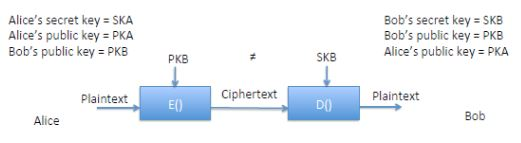
\includegraphics[width=12cm]{img/crittas.JPG}
\end{figure}

Gli algoritmi a chiave pubblica sono basati su esponenzializzazione modulari e sono molto più lenti da eseguire, data la loro complessità computazionale.

\subsection{Firma digitale}
La firma digitale è un'equivalente della firma scritta. Una funzione permette di firmare tramite una chiave privata. Il prodotto della funzione è proprio una firma, che può essere pubblicata.

Per verificare l'autenticità della firma, si utilizza una funzione booleana che verifica l'autenticità tramite la chiave pubblica del firmatario. Se una firma non risulta autentica, significa che è stata soggetta ad un attacco. 

\begin{figure}[htb]
\centering
  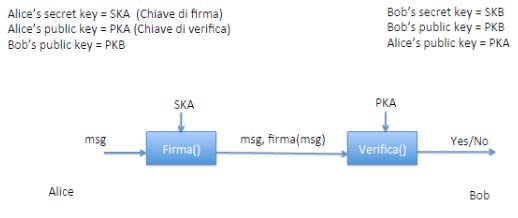
\includegraphics[width=12cm]{img/firma.JPG}
\end{figure}

La firma garantisce anche l'integrità del documento, in quanto per ogni modifica viene generata una nuova firma.

Gli algoritmi a chiave pubblica famosi sono diversi, fra tutti si ricordano RSA e DSA.
\newpage

\subsection{Autenticità del Sistema Operativo}
Un problema noto di un sistema operativo è quello di verificare che la versione del kernel sia originale e non modificata, magari con un malware all'interno. Per far ciò, esiste un chip ``sicuro'' integrato nella scheda madre, chiamato Trusted Platform Module (TPM). Questo chip fornisce la generazione e la memorizzazione sicura delle chiavi crittografiche. Dunque, si serve al software per l'implementazione di primitive crittografiche.

Quando il PC viene acceso (boot), parte il BIOS che inizializza l'hardware. Il BIOS invoca il codice memorizzato nel master boot record (MBR) presente nel disco. Ogni partizione ha un bootsector che viene caricato dall'MBR. Questo carica il codice dal bootsector ed esegue il bootloader dal file system. Il master boot record ha l'hash del bootsector corretto e lo confronta con il valore di hash che è memorizzato. Questa operazione viene ripetuta per tutti gli step fino al caricamento del kernel.

\begin{figure}[htb]
\centering
  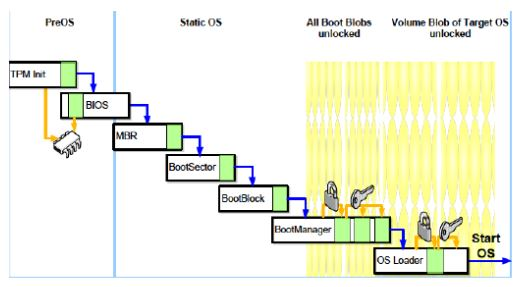
\includegraphics[width=12cm]{img/autso.JPG}
\end{figure}

Tutti i sistemi operativi implementano la cifratura del disco: quando viene spenta la macchina, il disco viene interamente cifrato per poi essere decifrato all'accensione successiva. La cifratura avviene tramite una chiave apposita, chiamata Storage Root Key (SRT), memorizzata nella TPM. La SRK viene utilizzata per cifrare la chiave di cifratura (FVEK -- Full Volume Encryption Key) dell'intero volume, la quale è memorizzata all'interno del disco.

In realtà, la cifratura e la decifratura avvengono incrementalmente, così da non rallentare troppo l'accensione e lo spegnimento.

\subsection{Sistema di autenticazione utenti}
Tutti i sistemi operativi forniscono una parte del kernel per aggiudicare l'accesso agli utenti. Il sistema operativo deve sapere chi accede, in quanto è fondamentale ai fini della sicurezza. Esistono diversi tipi di autenticazione dell’utente. Qui, verrà analizzato
solo quello basato su password testuali, ma è importante sapere che è possibile fare autenticazione tramite altro hardware che l’utente può possedere, come una smart card o una chiavetta usb, o tramite quello che l’utente è o fa, come può essere una caratteristica fisiologica o comportamentale (biometrica). 

L’autenticazione è composta da due step. Il primo passo consiste nell'identificazione, dove l’utente annucia la sua persona (per esempio con la richiesta di un username), mentre il secondo passo consiste nell’autenticazione, cioè la verifica vera e propria dove si controlla se effettivamente l'utente è chi dice di essere. Esistono delle regole teoriche da seguire per poter effettuare la scelta della password: tipicamente devono avere almeno 8 caratteri, dove è presente almeno una lettera minuscola, una lettera maiuscola, cifre numeriche e caratteri speciali. Esistono anche delle regole di rinnovo delle password, dove ogni \textit{tot} mesi è necessario modificarla. 

La memorizzazione della password è sicuramente un'operazione che deve essere accurata. La prima assunzione che occorre fare è che la password debba essere cifrata prima di venire salvata, in modo tale da evitare il problema di una lettura quando il sistema è accessibile. Questo sistema però non risolve nulla, in quanto un malware potrebbe utilizzare la chiave in chiaro in RAM per poter decifrare la password e accedere. 

Un sistema migliore è quello di memorizzare l’hash della password, in modo tale da confrontarla con la password immessa e accedere solo nel caso in cui entrambe coincidano. 

Un attacco possibile per individuare la password corretta sarebbe l'attacco a dizionario, dove vengono confrontate una serie di
parole fino a che non si trova la giusta hash.
 
 \subsection{Malware}
 Con malware si intende una categira molto ampia di software. Quando un sistema operativo non è progettato per un controllo di una funzionalità, esiste una vulnerabilità dell'intero sistema che può essere sfruttata da un malware. Tecniche di protezione di indirizzi di memoria e l'interposizione tra utente e hardware da parte del kernel sono due principi fondanti della sicurezza di un sistema operativo.

Questi principi in realtà sono costantemente in pericolo. I malware infatti tentano di violare una proprietà del sistema per poter accedere a risorse a cui non dovrebbero poter accedere, ottenendo quindi l'abilità di svolgere funzionalità altrimenti non permesse.

\subsubsection{Breve panoramica sui principali tipi di virus}
I \textbf{Trojan horse} sono tra i primi malware ad essere utilizzati e sono programmi che replicano funzionalità legittime, nascondendo però qualcosa di malevolo all'utente. Altra categoria di malware sono i \textbf{Keylogger}, ovvero dei programmi che si interpongono tra la tastiera e il sistema operativo, tentando di spedire all'attaccante tutto ciò che l'utente digita con la tastiera. La tastiera inserisce i caratteri in un buffer e il processo utente (in foreground) può consumare il buffer. Questa sciocca vulnerabilità esiste in quanto permette l'implementazione di shortcut da parte dei sistemi. I \textbf{Ransomware} sono malware che hanno privilegi di root, rendendo impossibile l'accesso al computer, magari bloccando l'accesso ai dati (cifrati) e ricattando l'utente per ripristinare la situazione. Si installa nei vari programmi di bootloader ottenendo così la persistenza. Generalmente, i \textbf{rootkit} ottengono la modalità kernel facendo puntare la tabella delle sys call al codice malevolo. La rimozione di un rootkit è garantita solo con la reinstallazione dell'intero sistema operativo. Uno \textbf{Worm} è una versione di un virus che si propaga in maniera molto veloce tramite la rete.

\subsection{Le vulnerabilità}
Il mondo dei malware esistono sfruttando vulnerabilità del sistema operativo. Una vulnerabilità è causata dal buffer overflow, ovvero la corruzione della memoria per poter inserire codice eseguibile. Il buffer è un blocco di memoria che contiene una o più istanze di dati. Esso ha una dimensione prefissata.

L'overflow di un buffer consiste proprio nello sforare la dimensione del buffer, in modo tale da sovrascrivere anche in aree di memoria non autorizzate. Ovviamente, ciò accade solo perché in un esiguo numero di software avvengono controlli di buffering.
 







\end{document}